% \documentclass[10pt,letterpaper,twocolumn]{article}
\documentclass[lettersize,journal]{IEEEtran} 

% Standalone two-column layout for the arXiv version (no conference template).
\usepackage[letterpaper,margin=0.75in,columnsep=0.25in]{geometry}
\usepackage[T1]{fontenc}
\usepackage[utf8]{inputenc}

\usepackage[hyphens]{url}  
\usepackage{graphicx}
\urlstyle{rm} 
\def\UrlFont{\rm} 
\usepackage{natbib}
\usepackage{caption} 
\frenchspacing
\usepackage{amsmath}
\usepackage{amssymb}
\usepackage{amsfonts}
\usepackage{amsthm}
\usepackage{subcaption}
\usepackage{booktabs}
\usepackage{array}
\usepackage{multirow}
\usepackage{pifont}
\usepackage[table]{xcolor}
\usepackage{algorithm}
\usepackage{algorithmic}
\usepackage{xr}
\usepackage[hidelinks]{hyperref}

% Resolve references to tables and figures moved to appendix.tex when appendix.aux exists.
\IfFileExists{appendix.aux}{\externaldocument{appendix}}{}

% Theorem environments.
\newtheorem{theorem}{Theorem}
\newtheorem{lemma}{Lemma}
\newtheorem{assumption}{Assumption}
\newtheorem{remark}{Remark}
\newtheorem{corollary}{Corollary}


\hypersetup{
	pdftitle={Rethinking Factor Sharing in Federated LoRA: A Rank-Aware Adaptive Approach},
    % pdftitle={FedAS-LoRA: Adaptive Factor Sharing for Federated Low-Rank Adaptation},
	pdfauthor={Xinyi Xu, Bingnan Xiao, Shuang Qin, Gang Feng, and Tony Q.S. Quek}
}

\setcounter{secnumdepth}{3}

% \title{FedAS-LoRA}
\title{Rethinking Factor Sharing in Federated LoRA: A Rank-Aware Adaptive Approach}
% \title{FedAS-LoRA: Adaptive Factor Sharing for Federated Low-Rank Adaptation}
% \author{Anonymous Submission}

\author{
Xinyi Xu\textsuperscript{1,*}\quad
Bingnan Xiao\textsuperscript{2,*}\quad
Shuang Qin\textsuperscript{1,\textdagger}\quad
Gang Feng\textsuperscript{1}\quad
Tony Q.S. Quek\textsuperscript{3}\\[0.5em]
\small \textsuperscript{1}University of Electronic Science and Technology of China\\
\small \textsuperscript{2}Fudan University\\
\small \textsuperscript{3}Singapore University of Technology and Design\\[0.25em]
\small \textsuperscript{*}Equal contribution.\quad
\textsuperscript{\textdagger}Corresponding author.\\[0.25em]
\small \texttt{xinyixu@std.uestc.edu.cn, 22110720061@m.fudan.edu.cn, blueqs@uestc.edu.cn}\\
\small \texttt{fenggang@uestc.edu.cn, tonyquek@sutd.edu.sg}
}
\date{}


\begin{document}
	
	\maketitle
	
	\begin{abstract}
		Low-rank adaptation (LoRA) represents large language model (LLM) updates with two compact matrix factors, i.e., $A$ and $B$, providing an efficient way to fine-tune large models in federated learning paradigm. 
		Inspired by the asymmetric roles of the LoRA factors, we study whether $A$ should be shared across clients while $B$ remains client-specific (Share-A/Local-B), or whether $B$ should instead be shared while $A$ remains client-specific (Share-B/Local-A).
		%Inspired by the asymmetric roles of the two LoRA factors, we study which LoRA factor should be shared across clients and which should remain client-specific.
		% With a least-squares surrogate, we reveal that Share-A/Local-B requires the client adaptations to use a common rank-$r$ input-side space, whereas Share-B/Local-A requires a common rank-$r$ output-side space. The resulting projection characterization shows that neither sharing policy is uniformly preferable: the preferred policy is determined by which common space yields the smaller aggregate residual across clients.
		% {\color{red}Using a least-squares surrogate, we show that Share-A/Local-B and Share-B/Local-A impose rank-$r$ constraints on the input and output sides of the client adaptations, respectively. These constraints yield projection residuals on different sides of the adaptations; within the surrogate, the preferred strategy is the one with the smaller mean squared residual across clients.}
		With a least-squares surrogate, we reveal that Share-A/Local-B requires the client-specific LoRA update matrices to use a common rank-$r$ input-side space, whereas Share-B/Local-A requires a common rank-$r$ output-side space. 
		The two strategies therefore incur different projection residuals, indicating that the preferred strategy is the one with the smaller aggregate residual across clients. 
		% \textbf{we investigate how their structure should reveal the division of shared and client-specific adaptation across clients. }
		% \textbf{Specifically, through a least-squares surrogate, we show that Share-A/Local-B imposes a common rank-$r$ input-side representation, whereas Share-B/Local-A imposes a common rank-$r$ output-side representation. 
			% {\color{red}can we state the following point based on this?}
			% This asymmetry indicates that the suitable sharing side depends on which side admits sufficient cross-client commonality under the client data partition and target LoRA rank. }
		With this insight, we propose Federated Adaptive Factor Sharing Low-Rank Adaptation (FedAS-LoRA), which selects the sharing side before training to enhance fine-tuning performance. 
		To enable adaptive factor selection before training, we design a Rank-Aware Shared-Subspace Sufficiency (RSS) metric, which effectively assesses whether a shared rank-$r$ input subspace is sufficient for the local data distributions using representations extracted from a frozen LLM backbone. 
		Experiments across different tasks, data distributions, LoRA ranks, and participation settings confirm the effectiveness of RSS and the superior performance of FedAS-LoRA.
	\end{abstract}
	
	
	
	\section{Introduction}
	Large language models (LLMs) have demonstrated strong capabilities in language understanding and generation, supporting a wide range of natural language processing applications~\cite{brown2020language,touvron2023llama}. For pretrained LLMs, task-specific adaptations are needed before deployment to meet the requirements of different scenarios~\cite{houlsby2019parameter,li2021prefix,hu2022lora}. In many practical settings, the data required for fine-tuning are distributed across clients or organizations and cannot be centralized due to privacy, ownership, or regulatory constraints. Federated learning (FL) enables multiple clients to collaboratively 
	fine-tune a model without sharing their private data~\cite{mcmahan2017communication,li2020federated}. Nevertheless, full-model fine-tuning in FL incurs substantial computation, storage, and communication costs. Parameter-efficient fine-tuning provides a practical alternative by updating only a small set of additional parameters~\cite{he2022towards}. In particular, low-rank adaptation (LoRA) keeps the pretrained LLM backbone frozen and represents each model update by two trainable low-rank factors, making it well suited to resource-constrained federated adaptation.
	
	
	One critical challenge of federated LoRA lies in aggregation mismatch. For 
	an FL system with $N$ clients, let the LoRA update of client $i$ be $\Delta W_i=B_iA_i$. Independently averaging the two factors $B_i$ and $A_i$ at the server yields
	\begin{equation}
		\Big(
		\frac{1}{N}\sum_{i =1}^{N}B_i
		\Big)
		\Big(
		\frac{1}{N}\sum_{i =1}^{N}A_i
		\Big)
		\neq
		\frac{1}{N}\sum_{i =1}^{N}B_iA_i,
		\label{eq:aggregation_mismatch}
	\end{equation}
	which differs from directly averaging the client model updates. Several studies have explored methods to address this mismatch~\cite{bian2025lorafair,wang2026iflora,chen2026fedotab}. One representative line of work assigns asymmetric training and aggregation roles to the two LoRA factors. For example, FFA-LoRA fixes a common randomly initialized factor $A_0$, and only trains and aggregates $B_i$~\cite{sun2024improving}. FedSA-LoRA instead keeps both factors trainable, aggregates $A_i$, and retains $B_i$ locally for personalized adaptation~\cite{guo2025selective}. Although such methods adopt different factor-handling strategies, they hard-code
	the roles of $A$ and $B$ before training and apply the same assignment across diverse system settings. 
	\textit{It remains unclear whether this hard-coded assignment is consistently superior, prompting a reconsideration of the roles of the LoRA factors B and A in federated settings.
	}
	
	\begin{figure}[t]
		\centering
		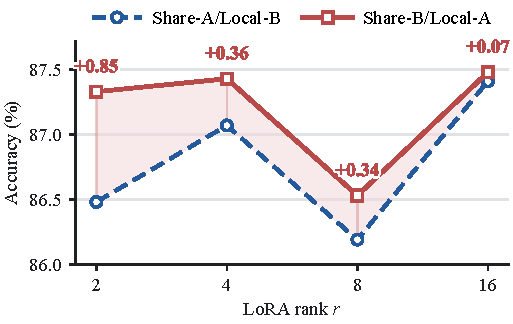
\includegraphics[width=0.95\linewidth]{mnli_genre3.pdf}
		\caption{Accuracy gap between Share-A/Local-B and Share-B/Local-A on the MNLI-m task under label-balanced input skew. 
			% from the server evaluation at the best-validation round under label-balanced input skew. 
			The federated system includes 3 clients with full participation and 500 training rounds. 
			% The focused y-axis makes the policy gap visible across LoRA ranks.
		}
		\label{fig:motivation_mnli_rank}
	\end{figure}
	% \textit{It remains unclear whether such a fixed assignment is consistently preferable under different client data partitions and LoRA ranks, or whether the roles of the two factors should adapt to the federated setting.}
	
	To examine this question, we compare Share-A/Local-B and Share-B/Local-A under a label-balanced input-skew partition. As shown in Fig.~\ref{fig:motivation_mnli_rank}, Share-B/Local-A outperforms Share-A/Local-B, and the performance gap varies with LoRA rank. This observation does not imply that Share-B/Local-A is always preferable. Instead, it means that fixing a sharing side is unsuitable for all federated LoRA settings. 
	We further analyze the structural asymmetry of the two LoRA factors through a least-squares surrogate. 
	The resultant projection characterization shows that sharing $A$ imposes a common rank-$r$ input-side representation across clients, whereas sharing $B$ imposes a common rank-$r$ output-side representation. Thus, the hard-coded sharing side assignment is not globally optimal, since
	% neither factor has a universally fixed global or local role. 
	the appropriate shared factor depends on whether a common rank-$r$ input-side or output-side space yields a smaller aggregate projection residual across clients.
	
	\begin{figure*}[t]
		\centering
		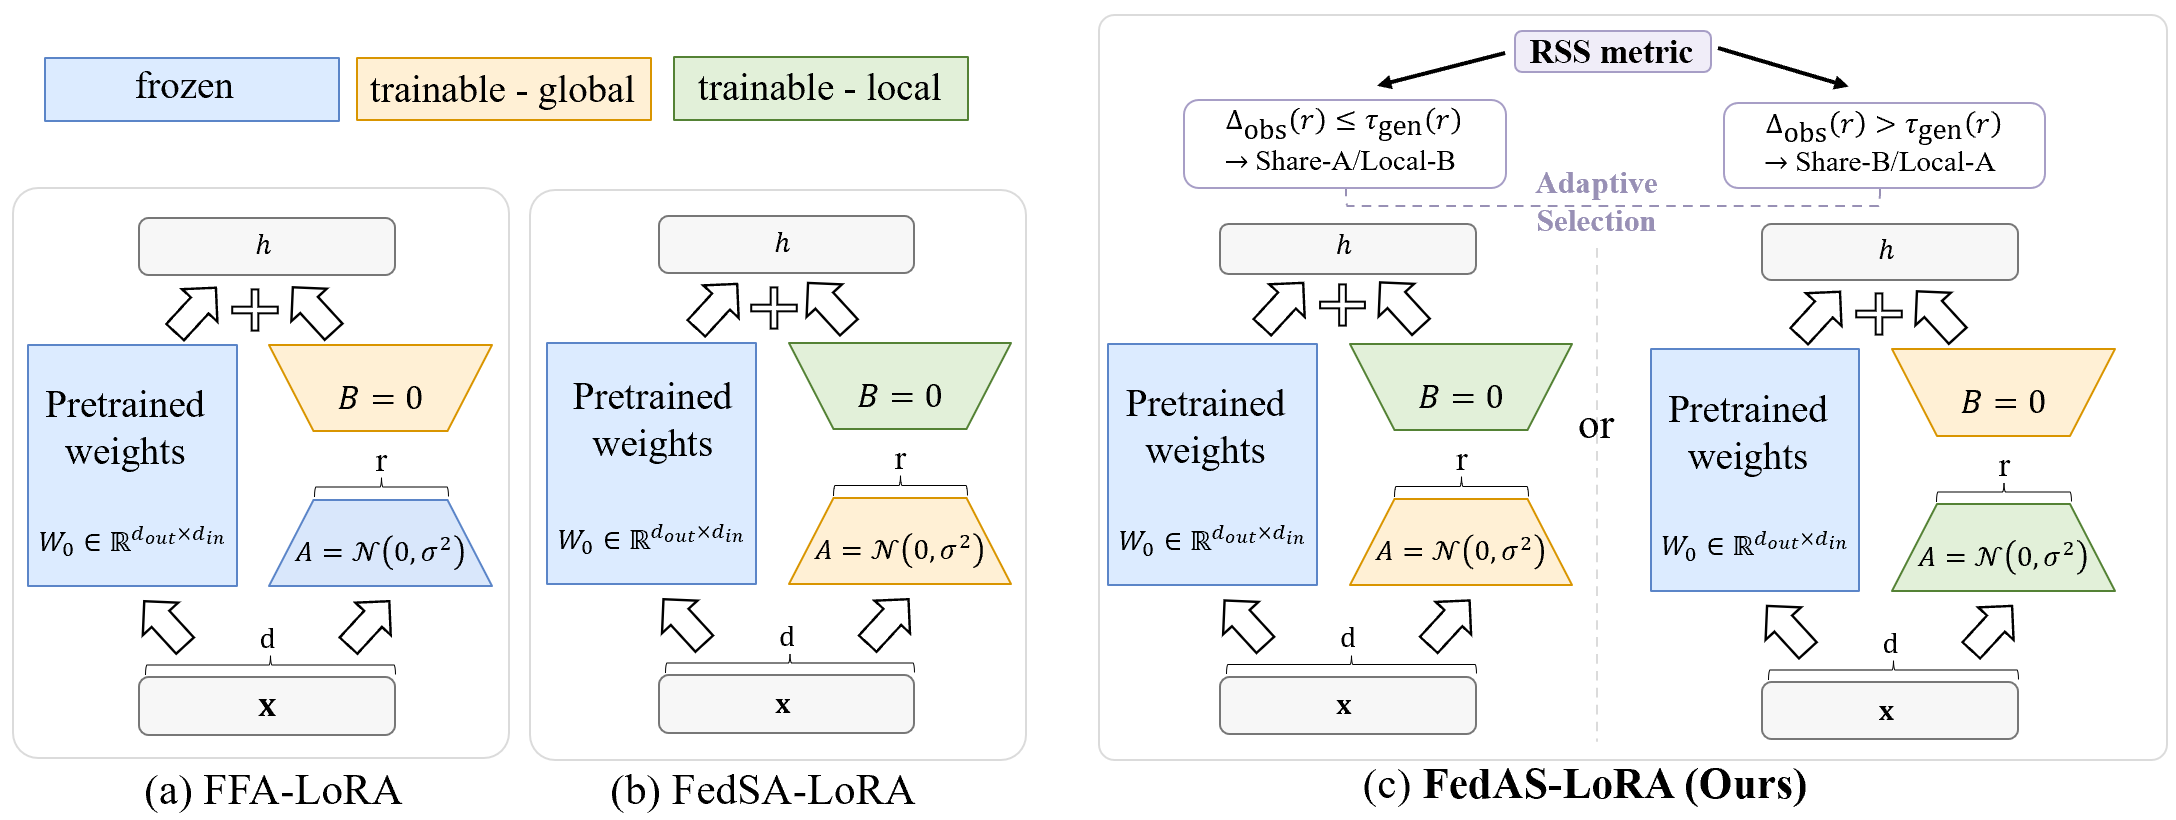
\includegraphics[width=0.85\textwidth]{sysmodel.png}
		\caption{Illustration of (a) FFA-LoRA, (b) FedSA-LoRA, and (c) FedAS-LoRA. 
			% The pretrained weights are frozen in all three methods. 
			In FFA-LoRA, $A$ is fixed after initialization, while $B$ is trainable and shared with the server for aggregation. In FedSA-LoRA, both $A$ and $B$ are trainable, while $A$ is shared and $B$ is retained locally. In FedAS-LoRA, the server uses RSS to determine the sharing strategy before training. For either strategy, both factors are updated locally; each client uploads only the shared factor and retains the other factor locally.}
		\label{fig:systemmodel}
	\end{figure*}
	
	Based on this insight, we propose Federated Adaptive Factor Sharing Low-Rank Adaptation (FedAS-LoRA) framework, as illustrated in Fig.~\ref{fig:systemmodel}. FedAS-LoRA adaptively selects the shared factor before training instead of hard-coding the same policy. To guide this selection, we design a Rank-Aware Shared-Subspace Sufficiency (RSS) metric using sequence-level representations extracted from a frozen LLM backbone. 
	RSS compares the second-order variation captured by a global rank-$r$ input subspace with that captured by the corresponding client-specific subspaces. 
	When the RSS deficit exceeds the calibrated threshold, FedAS-LoRA treats the global rank-$r$ input subspace as insufficient and selects Share-B/Local-A; otherwise, it selects Share-A/Local-B.
	We further establish that FedAS-LoRA converges to a stationary neighborhood under arbitrary client participation.
	
	Our main contributions are summarized as follows:
	\begin{itemize}
		\item 
		%We provide the first projection-based characterization of factor sharing in federated LoRA. 
		We provide the first projection-based comparison between Share-A/Local-B and Share-B/Local-A in federated LoRA.
		We reveal that Share-A/Local-B and Share-B/Local-A yield input-side and output-side projection residuals, respectively, which explains why fixed sharing strategies are not suitable for all federated settings.
		
		\item Based on this insight, we design an RSS metric to efficiently determine the shared factor before training. With RSS, we propose FedAS-LoRA, which adapts different federated settings to enhance fine-tuning performance.
		
		\item We prove the convergence of FedAS-LoRA under arbitrary client participation, extending the analysis beyond the full-participation setting.
		For either Share-A/Local-B or Share-B/Local-A strategy, we prove that the corresponding iterates converge to a stationary neighborhood.
		
		\item  Extensive experiments on diverse natural language tasks demonstrate the superiority of FedAS-LoRA over other methods, and validate the effectiveness of RSS-based adaptive sharing side selection.
	\end{itemize}
	%Large language models (LLMs) have demonstrated strong capabilities in
	% language understanding and generation, supporting a growing range of
	% natural language processing applications
	% \cite{brown2020language,touvron2023llama}. However, pretrained LLMs
	% often require task-specific adaptation to achieve reliable performance
	% for particular domains or deployment environments. In many settings,
	% the data required for adaptation are distributed across users or
	% organizations, while data centralization can be restricted by privacy,
	% ownership, and regulatory requirements. Federated learning (FL)
	% enables multiple clients to collaboratively optimize a model without
	% transferring raw local data to a central server, providing a natural
	% framework for adapting LLMs over decentralized datasets under
	% heterogeneous deployment conditions
	% \cite{mcmahan2017communication,li2020federated}.
	
	% Despite its promise, fine-tuning LLMs in an FL system remains
	% challenging due to the substantial computation and communication overhead required
	% at local clients. To enable
	% resource-efficient federated adaptation, various parameter-efficient
	% fine-tuning (PEFT) techniques have been explored. Representative
	% approaches include adapter-tuning-based methods
	% \cite{houlsby2019parameter}, prompt-tuning-based methods
	% \cite{li2021prefix}, and low-rank adaptation (LoRA)-based methods
	% \cite{hu2022lora}. Among these techniques, LoRA is particularly
	% appealing for FL because it keeps the pretrained backbone frozen and
	% optimizes only a small number of low-rank parameters for downstream
	% adaptation. Given these advantages, we focus on LoRA-based federated fine-tuning in this
	% work.
	
	% However, aggregating the LoRA matrices $A$ and $B$ in an FL
	% system poses a key problem. Consider an FL system with $N$
	% clients, independently averaging the two factors
	% at the server yields
	% \begin{equation}
		%     \left(\frac{1}{N}\sum_{i=1}^{N}B_i\right)
		%     \left(\frac{1}{N}\sum_{i=1}^{N}A_i\right)
		%     \neq
		%     \frac{1}{N}\sum_{i=1}^{N}B_iA_i,
		%     \label{eq:lora_aggregation_error}
		% \end{equation}
	% which causes aggregation mismatch. To solve this problem, some methods restrict
	% cross-client aggregation to one LoRA factor. For example,
	% FFA-LoRA fixes a common randomly initialized matrix $A_0$
	% and only updates and aggregates the $B_i$ matrices
	% \cite{sun2024improving}. Since all clients use the same $A_0$,
	% the aggregated update satisfies
	% $\left(\frac{1}{N}\sum_i B_i\right)A_0
	% =\frac{1}{N}\sum_i B_iA_0$. However, fixing $A_0$ reduces
	% the trainable degrees of freedom and may limit the adaptation
	% ability of LoRA. Meanwhile, prior studies have demonstrated
	% that enforcing a uniform model update for all clients can be
	% suboptimal, particularly when local data are non-IID, which
	% motivates the development of personalized FL
	% \cite{dinh2020personalized,collins2021exploiting}. In this
	% direction, FedSA-LoRA keeps both LoRA factors trainable,
	% shares the $A_i$ matrices with the server, and retains $B_i$
	% locally, based on the interpretation that $A$ captures general
	% knowledge while $B_i$ models client-specific knowledge
	% \cite{guo2025selective}. Although these methods are motivated
	% by different considerations, they both prescribe an asymmetric
	% factor-handling policy before federated training. Importantly, existing methods have assigned specific roles to the two LoRA factors before federated training. Although these assignments are motivated by
	% different considerations, the selected sharing side remains
	% fixed once each method is specified. To examine whether such
	% a fixed assignment remains suitable under different federated
	% settings, we compare Share-A/Local-B and Share-B/Local-A
	% on MNLI-m using RoBERTa-large and a three-client,
	% label-balanced input-skew partition
	% \cite{liu2019roberta,wang2018glue}. As shown in
	% Fig.~\ref{fig:motivation_mnli_rank}, Share-B/Local-A
	% achieves higher test accuracy across the evaluated ranks,
	% showing that the fixed Share-A/Local-B policy adopted by
	% FedSA-LoRA can be suboptimal under this client partition. It suggests that the appropriate sharing
	% side can vary with the client data partition and the target
	% LoRA rank. Therefore, we revisit the structural roles of the
	% two factors and seek a more adaptive way to integrate LoRA
	% with FL, rather than fixing their global and local roles in
	% advance.
	
	
	% To address this question, we start by analyzing the structural
	% asymmetry between the two LoRA factors in federated adaptation.
	% As formalized in
	% Theorem~\ref{thm:projection_characterization},
	% Share-A/Local-B and Share-B/Local-A impose projection
	% constraints on opposite sides of the client-specific target
	% updates. Specifically, sharing $A$ restricts all clients through
	% a common input-side mapping, which induces a
	% covariance-weighted right-side subspace constraint, while each
	% local $B_i$ remains free to produce client-specific output
	% transformations. In contrast, sharing $B$ enforces a common
	% output-side column space, while each local $A_i$ can preserve
	% a client-specific input representation. This analysis shows
	% that the two LoRA factors do not have universally fixed global
	% or local roles. Instead, the appropriate sharing policy depends
	% on which side of the client adaptations admits a common
	% rank-$r$ representation. The side exhibiting sufficient
	% cross-client commonality should be shared, whereas the side
	% requiring client-specific variation should remain local.
	% Therefore, the preferred sharing side is jointly determined by
	% the client-specific target adaptations, the input geometry, and
	% the target LoRA rank, rather than by data heterogeneity alone.
	
	% Based on these findings, we introduce the Federated Adaptive
	% Factor Sharing Low-Rank Adaptation (FedAS-LoRA) framework.
	% FedAS-LoRA retains the communication-efficient asymmetric
	% one-factor-sharing structure, but removes the assumption that
	% the same LoRA factor should always assume the global role.
	% Instead, it determines the sharing policy for each client data
	% partition and target LoRA rank before federated training. Since
	% the client-specific target adaptations in
	% Theorem~\ref{thm:projection_characterization} are unavailable
	% before fine-tuning, we design a rank-aware shared-subspace
	% sufficiency metric (RASS) based on frozen backbone
	% representations. RASS compares the representation energy
	% captured by a global rank-$r$ input subspace with that captured
	% by the client-specific rank-$r$ subspaces, and calibrates the
	% observed deficit against random-split and bootstrap baselines.
	% When the global input subspace is insufficient beyond the
	% calibrated noise level, FedAS-LoRA selects Share-B/Local-A,
	% allowing each client to retain its input-side factor $A_i$.
	% Otherwise, it adopts Share-A/Local-B as a conservative policy.
	% After the sharing side is selected, both LoRA factors remain
	% trainable during local fine-tuning, while only the selected
	% shared factor is communicated and aggregated. In this way,
	% FedAS-LoRA extends fixed one-factor aggregation to adaptive
	% factor sharing without requiring LoRA warm-up or
	% validation-based policy search.
	% However, aggregating the LoRA matrices $A$ and $B$ in an FL
	% system poses a key problem. Consider an FL system with $N$
	% clients, averaging the two factors
	% at the server produces aggregation mismatch
	% \begin{equation}
		%     \left(\frac{1}{N}\sum_{i=1}^{N}B_i\right)
		%     \left(\frac{1}{N}\sum_{i=1}^{N}A_i\right)
		%     \neq
		%     \frac{1}{N}\sum_{i=1}^{N}B_iA_i.
		%     \label{eq:lora_aggregation_error}
		% \end{equation}
	
	%  To address
	% this problem, several methods have been explored. For example,
	% FFA-LoRA fixes a common randomly initialized matrix $A_0$
	% and only updates and aggregates the $B_i$ matrices
	% \cite{sun2024improving}. Since all clients use the same $A_0$,
	% the aggregated update satisfies
	% $\left(\frac{1}{N}\sum_i B_i\right)A_0
	% =\frac{1}{N}\sum_i B_iA_0$. However, fixing $A_0$ reduces
	% the trainable degrees of freedom and can limit the adaptation
	% ability of LoRA. Meanwhile, prior studies have shown that
	% enforcing the same model update for all clients may be
	% suboptimal, particularly when local data are non-IID, which
	% motivates the development of personalized FL
	% \cite{dinh2020personalized,collins2021exploiting}. In this
	% direction, FedSA-LoRA keeps both factors trainable, shares the
	% $A_i$ matrices with the server, and retains $B_i$ locally,
	% based on the interpretation that $A$ captures general knowledge
	% while $B_i$ models client-specific knowledge
	% \cite{guo2025selective}. Although FFA-LoRA and
	% FedSA-LoRA are motivated by different considerations, both
	% prescribe the roles of the two LoRA factors before federated
	% training. To
	% examine whether such fixed assignments are always appropriate,
	% we compare Share-A/Local-B and Share-B/Local-A on MNLI-m
	% using RoBERTa-large and a three-client, label-balanced
	% input-skew partition
	% \cite{liu2019roberta,wang2018glue}. As shown in
	% Fig.~\ref{fig:motivation_mnli_rank}, Share-B/Local-A achieves
	% higher test accuracy across the evaluated ranks.
	% This result challenges the universality of the fixed role
	% assignment adopted by FedSA-LoRA and suggests that the
	% preferred sharing side can depend jointly on the client data
	% partition and the target LoRA rank. Therefore, it is necessary
	% to revisit the structural roles of the two factors and seek a more adaptive way to integrate LoRA with FL, rather than
	% fixing their global and local responsibilities in advance.
	
	
	% We start by analyzing
	% the structural asymmetry between the two LoRA factors in federated
	% adaptation. As formalized in
	% Theorem~\ref{thm:projection_characterization} shows that
	% Share-A/Local-B and Share-B/Local-A constrain opposite sides of the
	% client-specific target updates. Sharing $A$ imposes a
	% covariance-weighted right-side, or input-side, subspace constraint,
	% while local $B_i$ allows client-specific output transformations.
	% Conversely, sharing $B$ imposes a common left-side, or output-side,
	% column-space constraint, while local $A_i$ allows client-specific
	% input representations. Thus, neither factor has an inherently global
	% or local role. The suitable policy is to share the side that admits a
	% common rank-$r$ representation and keep the side requiring
	% client-specific variation local. This choice depends jointly on the
	% target adaptations and client input geometry, rather than on data
	% heterogeneity alone.
	
	% Based on these findings, we introduce the Federated Adaptive Factor Sharing
	% Low-Rank Adaptation (FedAS-LoRA) framework. Our key argument is that
	% prescribing either Share-A/Local-B or Share-B/Local-A as a universally
	% suitable policy provides an incomplete view of federated LoRA. Rather
	% than assigning fixed global and local roles to $A$ and $B$, FedAS-LoRA
	% treats the sharing side as a setting-dependent decision that accounts
	% for the client data partition and the target LoRA rank. We design a rank-aware shared-subspace sufficiency metric (RASS)
	% from frozen backbone representations. Once the sharing side is
	% determined, both factors remain trainable during local adaptation,
	% while only the selected shared factor is communicated and aggregated.
	% In this way, FedAS-LoRA provides a more adaptive integration of LoRA
	% and FL without requiring LoRA warm-up or validation-based policy
	% search.
	
	
	% Federated learning provides a practical way to adapt models from decentralized data without collecting raw client examples at a central server. This setting is increasingly relevant for language-model applications, where task data may be distributed across users, organizations, or deployment environments. However, federated fine-tuning of large pretrained language models is expensive: clients must optimize large models locally, and each communication round may require transmitting high-dimensional updates. Parameter-efficient fine-tuning addresses this bottleneck by updating only a small set of trainable parameters while keeping the pretrained backbone frozen. Low-rank adaptation (LoRA) is particularly suitable for this setting because it represents the update of a target weight matrix as
	% \begin{equation}
		%     \Delta W_i = B_i A_i,
		% \end{equation}
	% where $A_i\in\mathbb{R}^{r\times d_{\mathrm{in}}}$ and $B_i\in\mathbb{R}^{d_{\mathrm{out}}\times r}$ are low-rank trainable factors for client $i$. This factorization reduces trainable parameters and communication cost, making federated LoRA a natural candidate for parameter-efficient FL.
	
	% The low-rank product also introduces a structural choice that does not arise in standard full-model aggregation. Personalization in federated learning can be realized through different model components and optimization mechanisms; factor sharing is one specific design dimension in federated LoRA. This work focuses on the asymmetric setting in which one LoRA factor is shared and the other remains client-specific. Existing methods typically instantiate this setting with a fixed assignment. A representative design is Share-A/Local-B, where the server maintains a shared $A$ and each client keeps $B_i$ local. Once this assignment is chosen, the global and local roles of the two factors remain unchanged across client partitions and LoRA ranks.
	
	% The unresolved question within this setting is whether the same factor should always play the global role. The two LoRA factors are not interchangeable: $A_i$ projects the input representation into a rank-$r$ latent subspace, whereas $B_i$ maps this low-rank representation back to the output side. Choosing Share-A/Local-B or Share-B/Local-A therefore determines which side of the adaptation must use a common subspace across clients. When client heterogeneity mainly appears in the input-side representation, sharing $A$ may be restrictive because clients can require different input subspaces even when their label distributions are similar. When a common input-side subspace is sufficient, Share-A/Local-B remains a conservative and communication-efficient choice. Thus, for asymmetric one-factor sharing, the assignment should depend on the client partition and target LoRA rank rather than being fixed in advance.
	
	% A motivating MNLI-m rank sweep isolates this issue. Under a label-balanced input-skew partition, Share-B/Local-A outperforms the representative Share-A/Local-B configuration across the evaluated ranks, but the performance gap changes substantially with $r$. This comparison does not rank personalization mechanisms in general, nor does it imply that Share-B/Local-A is universally preferable. Instead, it exposes a limitation of fixed asymmetric factor sharing: the preferred assignment can depend jointly on the client partition and the target rank. The resulting question is whether a given partition admits a shared rank-$r$ input subspace or requires client-specific input-side subspaces.
	
	% We first formalize the asymmetry between the two factors through a least-squares surrogate. The analysis shows that Share-A/Local-B and Share-B/Local-A impose projection bottlenecks on different sides of the client-specific update. Share-A/Local-B constrains the right-side, or input-side, subspace through the shared $A$, while leaving output-side transformations to local $B_i$. Share-B/Local-A constrains the left-side, or output-side, subspace through the shared $B$, while leaving input-side adaptation to local $A_i$. This view explains why a single sharing side can be suboptimal: the shared factor may be placed on the side where clients require local variation.
	
	% Based on this view, we propose RASS, a rank-aware shared-subspace sufficiency diagnostic for federated LoRA. RASS is computed before federated training from frozen RoBERTa-large CLS representations and the target rank. For each client, it estimates the covariance structure of frozen input representations and compares the energy explained by a global rank-$r$ subspace with the energy explained by the client's own best rank-$r$ subspace. If the global subspace explains nearly as much covariance energy as the local subspaces, the partition is treated as compatible with Share-A/Local-B. If the observed deficit exceeds calibration thresholds from random splits and bootstrap resampling, RASS selects Share-B/Local-A, keeping $A_i$ local. The diagnostic does not train LoRA factors, compute gradients, or use validation performance.
	
	% The resulting framework treats factor sharing as a pre-training selection problem. For each dataset, client partition, and LoRA rank, the method selects either Share-A/Local-B or Share-B/Local-A before federated optimization begins. This keeps the training protocol simple while avoiding a single fixed assignment within the asymmetric one-factor-sharing setting. It also makes the decision interpretable: a Share-B/Local-A decision means that one global input subspace is insufficient beyond calibration noise; a Share-A/Local-B decision means that the shared input subspace is sufficient or the diagnostic is uncertain.
	
	% Our contributions are as follows:
	% \begin{itemize}
		%     \item We formulate adaptive factor sharing within the asymmetric one-factor-sharing setting, showing that a fixed Share-A or Share-B assignment can be inadequate under heterogeneous client partitions.
		%     \item We provide a left/right subspace interpretation of LoRA factor sharing, identifying the different projection bottlenecks induced by Share-A/Local-B and Share-B/Local-A.
		%     \item We propose RASS, a rank-aware, training-free diagnostic that measures whether a global input-side subspace is sufficient for the client partition before federated training.
		%     \item We develop a RASS-guided federated LoRA framework with a stationary-neighborhood analysis under arbitrary client participation and evaluate whether the diagnostic predicts the better sharing side across GLUE tasks, partitions, and LoRA ranks.
		% \end{itemize}
	
	
	% \section{Related Work}
	% \label{sec:related_work}
	% {\color{black}
		% \textbf{Federated Parameter-Efficient Fine-Tuning.}
		% Parameter-efficient fine-tuning (PEFT) reduces the computation, memory, and communication costs of adapting pretrained models in federated learning. Existing studies incorporate prompt tuning and low-rank adaptation into federated training by optimizing only a small set of task-specific parameters~\cite{che2023federated,sun2024fedbpt,hu2022lora}. Personalized methods combine global and local adapters to capture shared and client-specific knowledge~\cite{yang2024dual}, while other studies support clients with heterogeneous LoRA ranks through rank-compatible aggregation~\cite{bai2024federated,wang2024flora}. These methods improve the efficiency and flexibility of federated PEFT, but generally treat each LoRA adapter as an integral module. They do not examine how the two factors within a LoRA update should divide the shared and client-specific roles.
		
		% \textbf{Asymmetric Factor Handling and LoRA Factor Asymmetry.}
		% Recent studies have revealed that the two factors in the LoRA update $BA$ exhibit different optimization and representation behaviors. LoRA-FA freezes $A$ and only trains $B$ to reduce memory consumption, while other analyses and asymmetric architectures further exploit the distinct roles of the two factors~\cite{zhang2023lorafa,zhu2024asymmetry,tian2024hydralora}. In federated learning, FFA-LoRA fixes a common randomly initialized $A$ and aggregates only $B$, whereas FedSA-LoRA trains both factors, shares $A$, and retains $B$ locally for personalization~\cite{sun2024improving,guo2025selective}. Although these methods demonstrate the benefit of factor-wise training and aggregation, they predetermine the roles of $A$ and $B$ across different client partitions and LoRA ranks. FedAS-LoRA instead characterizes Share-A and Share-B through their input- and output-side projection constraints and selects the sharing side before federated training.
		% }
	
	\section{Related Work}
	
	\subsection{Federated Parameter-Efficient Fine-Tuning}
	Parameter-efficient fine-tuning (PEFT) reduces the computation, memory, and communication costs of adapting pretrained models in federated learning. Existing studies apply prompt tuning and other compact trainable modules while keeping the pretrained backbone frozen \cite{che2023federated,sun2024fedbpt,guo2024promptfl}. Low-rank adaptation (LoRA) represents each weight update with two low-rank factors, making it suitable for federated fine-tuning with limited client resources.
	
	Existing federated LoRA methods mainly address personalization, resource heterogeneity, and aggregation error~\cite{yang2025fedlorasurvey,koo2025towards,byun2025towards,
		shen2025pfedgpt}. FedDPA maintains global and personalized adapters to capture shared and client-specific knowledge \cite{yang2024dual}. HetLoRA supports resource-heterogeneous clients through rank self-pruning and sparsity-weighted aggregation \cite{cho2024heterogeneous}, while FlexLoRA and FLoRA aggregate LoRA modules with different ranks through reconstruction or stacking \cite{bai2024federated,wang2024flora}. FedEx-LoRA instead corrects the mismatch between factor-wise averaging and direct averaging of the resulting updates \cite{singhal2025fedex}. These methods determine shared and personalized components at the adapter level, or improve the aggregation of heterogeneous LoRA updates. 
	
	
	\subsection{LoRA Factor Asymmetry and Factor-Wise Federated Aggregation}
	The two LoRA factors can exhibit different optimization and representation behaviors. LoRA-FA freezes $A$ and trains only $B$ to reduce the memory cost of fine-tuning \cite{zhang2023lorafa}, whereas LoRA+ assigns different learning rates to the two factors \cite{hayou2024loraplus}. Zhu et al.\ interpret $A$ as extracting input features and $B$ as mapping these features to the output space \cite{zhu2024asymmetry}. HydraLoRA further adopts an asymmetric architecture with a shared $A$ and multiple $B$ experts \cite{tian2024hydralora}. These studies establish factor asymmetry in centralized fine-tuning, but do not consider the division of shared and client-specific factors in federated learning.
	
	Factor-wise handling has also been explored in federated LoRA~\cite{chen2026fedotab,wang2026iflora,xu2025yoco}. FFA-LoRA fixes a common randomly initialized $A$ and trains and aggregates $B$ \cite{sun2024improving}. FedSA-LoRA trains both factors, shares $A$, and retains $B$ locally for personalization \cite{guo2025selective}. RoLoRA alternates the optimization of the two factors during federated training~\cite{chen2025rolora}, while FedRot-LoRA aligns client factors through orthogonal transformations before aggregation~\cite{zhang2026fedrotlora}. Although these methods assign different training or aggregation roles to the two factors, the sharing side is either predetermined or not explicitly considered. Which LoRA factor should be shared across clients and which should remain client-specific remains underexplored.
	% To be completed after the bibliography is finalized.
	% Suggested topics:
	% (1) Parameter-efficient fine-tuning and LoRA.
	% (2) Federated PEFT and personalized federated LoRA.
	% (3) Client heterogeneity and personalization in federated learning.
	% (4) Data heterogeneity diagnostics and adaptive FL strategies.
	
	
	\section{Preliminaries and Motivation}
	\label{sec:preliminaries}
	
	This section formulates the federated LoRA factor-sharing problem and proves that a fixed sharing side is insufficient. 
	We first define a general federated factor-sharing model covering Share-A, Share-B, and full-factor sharing, followed by a motivating example to illustrate that Share-B/Local-A can outperform Share-A/Local-B. 
	Based on a least-squares surrogate, we characterize the structural asymmetry between the two LoRA factors in federated settings.
	
	
	\subsection{Factor Sharing in Federated LoRA}
	\label{subsec:general_fed_lora_model}
	Consider a federated fine-tuning system with a server and $N$
	clients, indexed by $\mathcal{N}=\{1,2,\ldots,N\}$. Client $i$
	owns a local dataset $\mathcal{D}_i$ and optimizes a local
	objective $f_i$.
	For a target linear layer with frozen pretrained weight
	$W_0\in\mathbb{R}^{d_{\mathrm{out}}\times d_{\mathrm{in}}}$, the LoRA update of each client $i$ is $\Delta W_i=B_iA_i$. Here, $A_i\in\mathbb{R}^{r\times d_{\mathrm{in}}}$,
	$B_i\in\mathbb{R}^{d_{\mathrm{out}}\times r}$, and
	$r\ll\min\{d_{\mathrm{in}},d_{\mathrm{out}}\}$ denotes the LoRA
	rank. 
	Given an input representation
	$x\in\mathbb{R}^{d_{\mathrm{in}}}$, $A_i$ maps $x$ to an
	$r$-dimensional latent representation, while $B_i$ maps this
	representation to the output space.
	
	For federated LoRA settings, we consider a fixed shared factor type $Q\in\{A,B\}$. Let $Q_i=A_i$ when $Q=A$ and
	$Q_i=B_i$ when $Q=B$ for brevity. The corresponding personalized
	federated objective is
	\begin{equation}
		\begin{aligned}
			\min_{\{A_i,B_i\}_{i=1}^{N}}
			\quad&
			\frac{1}{N}
			\sum_{i=1}^{N}
			f_i(B_iA_i)
			\\
			\mathrm{s.t.}\quad&
			Q_i=Q_j,
			\
			\forall i,j\in\mathcal{N}.
		\end{aligned}
		\label{eq:personalized_fedlora_objective}
	\end{equation}
	Here, $f_i(B_iA_i)$ denotes the local loss evaluated
	at $W_0+B_iA_i$. When $Q=A$, the constraint shares $A$
	across clients while leaving $B_i$ client-specific, yielding
	Share-A/Local-B. When $Q=B$, it shares $B$ while leaving
	$A_i$ client-specific, yielding Share-B/Local-A.
	At training round $t$, let $Q_t$ be the shared
	factor maintained by the server and $Q_{t,i}^{e}$ its local
	copy at participating client $i$ after $e$ local updates.
	% We analyze the factor-sharing branch selected by RASS after the sharing side is fixed. The proof follows the protocol in Section~\ref{subsec:general_fed_lora_model} and shows that the selected branch reaches a stationary neighborhood under arbitrary client participation, provided the realized sets $\mathcal{S}_t$ satisfy the gradient-mass coverage condition in Appendix~\ref{app:convergence_proof}.
	
	
	% Consider a federated fine-tuning system with a server and $N$ clients, indexed by $\mathcal{N}=\{1,2,\ldots,N\}$. Client $i$ owns a local dataset $\mathcal{D}_i$ and a local objective $f_i$. For a fixed sharing policy $\mathcal{Q}\in\{\{A\},\{B\}\}$, FedAS-LoRA solves
	% \begin{equation}
		% \begin{cases}
			% \displaystyle
			% \min_{A,\{B_i\}_{i=1}^{N}}
			% \frac{1}{N}
			% \sum_{i=1}^{N}
			% f_i(B_iA),
			% & \mathcal{Q}=\{A\},\\[7pt]
			% \displaystyle
			% \min_{B,\{A_i\}_{i=1}^{N}}
			% \frac{1}{N}
			% \sum_{i=1}^{N}
			% f_i(BA_i),
			% & \mathcal{Q}=\{B\},
			% \end{cases}
		% \label{eq:personalized_fedlora_objective}
		% \end{equation}
	% {\color{red}
		% Consider a federated fine-tuning system with a server and $N$
		% clients, indexed by $\mathcal{N}=\{1,2,\ldots,N\}$. 
		% Each client $i$
		% owns a local dataset $\mathcal{D}_i$, a local objective
		% $f_i$, and two LoRA factors, denoted by $A_i$ and $B_i$. 
		% Let $\mathcal{Q}\subseteq\{A,B\}$ denote the set of factor types shared through the server. For each $Q\in\mathcal{Q}$, $Q_t$ denotes the server-maintained shared factor at round $t$, and $Q_{t,i}^{e}$ denotes its local copy maintained by client $i$ at local step $e$.
		% Given a fixed one-factor sharing policy
		% $\mathcal{Q}\in\{\{A\},\{B\}\}$, FedAS-LoRA solves the
		% following consensus-constrained problem:
		% \begin{equation}
			% \begin{aligned}
				%     \min_{\{A_i,B_i\}_{i=1}^{N}}
				%     \quad&
				%     \frac{1}{N}
				%     \sum_{i=1}^{N}
				%     f_i(B_iA_i)
				%     \\
				%     \mathrm{s.t.}\quad&
				%     \Theta_i=\Theta_j,
				%     \qquad
				%     \forall i,j\in\mathcal{N},
				%     \quad
				%     \forall \Theta\in\mathcal{Q}.
				% \end{aligned}
			% \label{eq:personalized_fedlora_objective}
			% \end{equation}
		% where $f_i(U_i)$ denotes the local loss evaluated with the frozen pretrained weights $W_0$ and the LoRA-induced update $U_i$.
		% If $\mathcal{Q}=\{A\}$, the constraint
		% enforces $A_i=A_j$ for all clients while leaving $B_i$
		% client-specific, which gives Share-A/Local-B. If
		% $\mathcal{Q}=\{B\}$, it enforces $B_i=B_j$ while leaving
		% $A_i$ client-specific, which gives Share-B/Local-A.
		% RASS determines $\mathcal{Q}$ before federated training,
		% after which the selected sharing policy remains fixed.
		% RASS determines $\mathcal{Q}$ before federated training, after which the selected sharing policy remains fixed.
		
		% % Consider a federated fine-tuning system with a server and $N$ clients, indexed by $\mathcal{N}=\{1,2,\ldots,N\}$. Client $i$ owns a local dataset $\mathcal{D}_i$ and optimizes a local objective $f_i$. At training round $t$, let $U_{t,i}=B_{t,i}A_{t,i}$ denote the LoRA-induced product update of client $i$. {\color{red}We track the average personalized objective value at round $t$ as}
		% % % Since one LoRA factor remains client-specific, $U_{t,i}$ can differ across clients. We track the average personalized objective value at round $t$ as
		% % \begin{align}
			% %     F_t
			% %     =
			% %     \frac{1}{N}
			% %     \sum_{i=1}^{N}
			% %     f_i(U_{t,i}),
			% %     \label{eq:aggregate_objective_convergence}
			% % \end{align}
		% % where $f_i(U_{t,i})$ denotes the local loss of client $i$ evaluated with the frozen pretrained weights and its current LoRA update $U_{t,i}$. We assign equal weight to each client throughout the convergence analysis.
		
		% }
	
	
	
	
	
	
	% Consider a target linear layer with frozen pretrained weight $W_0\in\mathbb{R}^{d_{\mathrm{out}}\times d_{\mathrm{in}}}$. For client $i$, LoRA represents the trainable update by a low-rank product
	% \begin{equation}
		%     \Delta W_i = B_iA_i,
		%     \label{eq:lora_update_prelim}
		% \end{equation}
	% where $A_i\in\mathbb{R}^{r\times d_{\mathrm{in}}}$, $B_i\in\mathbb{R}^{d_{\mathrm{out}}\times r}$, and $r\ll\min\{d_{\mathrm{in}},d_{\mathrm{out}}\}$ is the LoRA rank.
	% {\color{red}Given an input representation $x\in\mathbb{R}^{d_{\mathrm{in}}}$, the LoRA-induced adaptation is $\Delta W_i x = B_iA_i x$. Thus, $A_i$ maps the input representation into an $r$-dimensional latent space, while $B_i$ maps this latent representation to the output side.}
	
	% A federated LoRA method specifies which LoRA factors are shared by the server and which factors remain client-local. Let $\mathcal{Q}\subseteq\{A,B\}$ denote the set of shared LoRA factors. The case $\mathcal{Q}=\{A\}$ corresponds to Share-A/Local-B, where the server maintains a shared $A$ and each client keeps its own $B_i$. The case $\mathcal{Q}=\{B\}$ corresponds to Share-B/Local-A, where the server maintains a shared $B$ and each client keeps its own $A_i$. The case $\mathcal{Q}=\{A,B\}$ corresponds to sharing both LoRA factors. We focus on nonempty $\mathcal{Q}$, since at least one shared factor is needed for cross-client collaboration.
	
	% The federated training workflow is common to all sharing policies. 
	In each training round $t$, the following steps are executed:
	\begin{itemize}
		\item \textbf{Client selection and downlink transmission:}
		The server selects an arbitrary subset of $\mathcal{S}_t\subseteq\mathcal{N}$ with $S_t$ clients, and broadcasts $Q_t$, $Q \in \{A,B\}$, to clients $i\in\mathcal{S}_t$.
		
		\item \textbf{Local update:}
		Each selected client initializes the local copy of every shared factor as $Q_{t,i}^{0}=Q_t$, and performs $E$ local update steps with local learning rate $\eta_\ell$ on its local dataset $\mathcal{D}_i$. During local training, the client updates all trainable LoRA factors in its local model, while keeping non-shared factors client-local.
		
		\item \textbf{Uplink Aggregation:}
		After local training, each selected client uploads the update of the shared factor, $\Delta Q_{t,i} \!=\! Q_{t,i}^{E} \!-\! Q_t, Q\in \{A,B \}$ to the server for aggregation:
		\begin{equation}
			Q_{t+1}
			=
			Q_t
			+
			\eta_g
			\frac{1}{S_t}
			\sum_{i\in\mathcal{S}_t}
			\Delta Q_{t,i},
			% \ Q\in\mathcal{Q},
			\label{eq:generic_server_average_update}
		\end{equation}
		where $\eta_g$ is the server learning rate.
	\end{itemize}
	The sharing strategy determines which side of the LoRA adaptation is exposed to cross-client averaging and which side remains client-specific. 
	% The rest of this work focuses on deciding between the two asymmetric policies $\mathcal{Q}=\{A\}$ and $\mathcal{Q}=\{B\}$, since they preserve one personalized LoRA factor while aggregating the other across clients.
	
	
	
	
	
	\subsection{Observation: Fixed Sharing Can Be Suboptimal}
	\label{subsec:motivation_study}
	
	One representative personalized federated LoRA design adopts Share-A/Local-B, i.e., sharing factor $A$ while keeping $B_i, \forall i \in \mathcal{N}$ client-specific in each training round~\cite{guo2025selective}. 
	% {\color{red}This assignment is reasonable when clients can use a common input-side subspace.
		% It can nevertheless be restrictive when the appropriate shared subspace changes with the client distribution or the LoRA rank.}  
	However, it remains unclear whether sharing $A$ is always preferable to sharing $B$.
	To  {\color{black}answer} this question, we compare Share-A/Local-B and Share-B/Local-A on MNLI-m~\cite{wang2018glue} using a label-balanced input-skew partition.
	% Specifically, we examine the training performance of Share-A/Local-B
	% and Share-B/Local-A on MNLI-m \cite{wang2018glue} with a label-balanced input-skew partition.
	% {\color{red}
		% For each data label, training examples are ordered by an input score constructed from premise--hypothesis length statistics, token overlap, and genre when available, and then divided evenly among the three clients. This construction produces nearly identical training-label histograms while inducing systematic differences in sentence-pair characteristics. Validation and test examples are assigned using label-specific tertile thresholds estimated from the training split.
		% Both Share-A/Local-B and Share-B/Local-A use consistent local data distribution, optimizer, and training budget, with only the shared LoRA factor differing. 
		% }
	{\color{black}{To create input skew while preserving label balance, we construct a three-client partition based on the genre annotations provided by MNLI~\cite{wang2018glue}. Each client is assigned premise--hypothesis pairs from one of three genres: telephone, government, and fiction. The partition is constructed such that the clients have nearly identical distributions over the three MNLI labels. Thus, the clients share the same prediction task and similar label distributions, while their inputs originate from different textual genres. This setting introduces genre-based input heterogeneity while controlling for label skew. }}
	Fig.~\ref{fig:motivation_mnli_rank} compares their test accuracies for $r\in\{2,4,8,16\}$.
	It is noted that Share-B/Local-A achieves better performance for all rank settings, while the accuracy advantage varies with the LoRA rank $r$, indicating that the performance difference between the two sharing strategies depends on the LoRA rank $r$.
	
	
	
	% Fig.~\ref{fig:motivation_mnli_rank} demonstrates that Share-A/Local-B is not uniformly optimal even when label imbalance is controlled. 
	% The observation motivates a rank-aware question: {\color{red}\textit{does the client partition admit a sufficiently expressive shared rank-$r$ input subspace, or should $A_i$ remain local?} }
	% We next answer this question by analyzing the structural asymmetry between the two LoRA factors.
	
	Fig.~\ref{fig:motivation_mnli_rank} demonstrates that Share-A/Local-B is not uniformly optimal across different FL settings. This observation motivates the following question: 
	{\color{black}\textit{For a given LoRA rank $r$ and client data distributions, what determines which factor should be shared and which should remain client-specific?}}
	We next examine this question by analyzing the structural asymmetry between the two LoRA factors.
	
	
	% \subsection{xxx}
	% \label{subsec:lora_structural_asymmetry}
	
	% The motivating result above points to a structural limitation
	% of fixed LoRA factor sharing: a factor that is suitable for
	% cross-client aggregation under one partition may become the
	% bottleneck under another. We study this limitation through a
	% single-layer least-squares surrogate, to represent the constraints introduced by sharing one LoRA factor across clients.
	
	% For client $i$, let
	% $\Delta_i\in\mathbb{R}^{d_{\mathrm{out}}\times d_{\mathrm{in}}}$
	% denote the desired adaptation.
	% For a rank-$r$ LoRA update $B_iA_i$, the corresponding population least-squares surrogate is 
	% \begin{align}
		%     \mathcal{L}_i(B_i,A_i)
		%     &=
		%     \mathbb{E}\!\left[
		%         \|(\Delta_i-B_iA_i)x_i\|_2^2
		%     \right] \notag\\
		%     &\overset{(a)}{=}
		%     \|(\Delta_i-B_iA_i)\Sigma_i^{1/2}\|_F^2,
		%     \label{eq:ls_surrogate_loss}
		% \end{align}
	% where $x_i\in\mathbb{R}^{d_{\mathrm{in}}}$ denotes the input feature, and $(a)$ comes from $\Sigma_i=\mathbb{E}[x_ix_i^\top]\succ0$.
	
	% {\color{red}
		% When both factors are local, each client can choose its own
		% rank-$r$ factorization without cross-client coupling.
		% Federated sharing introduces such coupling by requiring one
		% factor to be common to all clients. We therefore compare the
		% best average approximation errors under the two possible
		% coupling constraints:
		% \begin{align}
			%     \mathcal{E}_A
			%     &=
			%     \min_{A,\{B_i\}}
			%     \frac{1}{N}
			%     \sum_{i=1}^{N}
			%     \|(\Delta_i-B_iA)\Sigma_i^{1/2}\|_F^2,
			%     \label{eq:pa_surrogate}\\
			%     \mathcal{E}_B
			%     &=
			%     \min_{B,\{A_i\}}
			%     \frac{1}{N}
			%     \sum_{i=1}^{N}
			%     \|(\Delta_i-BA_i)\Sigma_i^{1/2}\|_F^2,
			%     \label{eq:pb_surrogate}
			% \end{align}
		% where $\mathcal{E}_A$ is the smallest error attainable when
		% $A$ is shared and $B_i$ remains local, whereas
		% $\mathcal{E}_B$ is the corresponding error when $B$ is
		% shared and $A_i$ remains local.
		
		% The quantities $\mathcal{E}_A$ and $\mathcal{E}_B$ determine
		% which strategy fits the client targets better, but they do not
		% yet reveal why the two constraints behave differently. That
		% difference becomes explicit after eliminating the local
		% factor. For any candidate shared factors $A$ and $B$, define
		% \begin{align}
			%     \Pi_{i,A}
			%     &=
			%     (A\Sigma_i^{1/2})^\top
			%     (A\Sigma_iA^\top)^\dagger
			%     (A\Sigma_i^{1/2}),
			%     \label{eq:pa_projector}\\
			%     \Pi_B
			%     &=
			%     B(B^\top B)^\dagger B^\top.
			%     \label{eq:pb_projector}
			% \end{align}
		% The projector $\Pi_{i,A}$ selects the covariance-weighted
		% input subspace accessible through the shared factor $A$ for
		% client $i$, whereas $\Pi_B$ selects the common output
		% subspace accessible through the shared factor $B$. Theorem
		% \ref{thm:projection_characterization} characterizes exactly
		% which components remain unrepresented after the corresponding
		% local factor is optimized.
		% }
	
	% \begin{theorem}
		% \label{thm:projection_characterization}
		% Assume that $\Sigma_i\succ0, \forall i \in \mathcal{N}$. {\color{red}Eliminating the
			% client-local factor in the two sharing strategies yields}
		% \begin{align}
			%     \mathcal{E}_A
			%     &=
			%     \min_A
			%     \frac{1}{N}
			%     \sum_{i=1}^{N}
			%     \left\|
			%         \Delta_i\Sigma_i^{1/2}(I-\Pi_{i,A})
			%     \right\|_F^2,
			%     \label{eq:pa_projection}\\
			%     \mathcal{E}_B
			%     &=
			%     \min_B
			%     \frac{1}{N}
			%     \sum_{i=1}^{N}
			%     \left\|
			%         (I-\Pi_B)\Delta_i\Sigma_i^{1/2}
			%     \right\|_F^2.
			%     \label{eq:pb_projection}
			% \end{align}
		% Thus, sharing $A$ leaves an irreducible right-projection
		% residual, while sharing $B$ leaves an irreducible
		% left-projection residual. At the prescribed LoRA rank,
		% Share-B/Local-A has the lower attainable surrogate error
		% exactly when $\mathcal{E}_B<\mathcal{E}_A$; Share-A/Local-B
		% has the lower error exactly when
		% $\mathcal{E}_A<\mathcal{E}_B$.
		% \end{theorem}
	% {\color{black}To obtain explicit conditions for strict sharing-side
		% preference, define the vertically stacked and horizontally
		% concatenated client target adaptations as
		% \begin{align}
			%     \Delta_{\mathrm{row}}
			%     &=
			%     \begin{bmatrix}
				%         \Delta_1\\
				%         \Delta_2\\
				%         \vdots\\
				%         \Delta_N
				%     \end{bmatrix}
			%     \in
			%     \mathbb{R}^{Nd_{\mathrm{out}}\times d_{\mathrm{in}}},
			%     \label{eq:delta_row_stack}\\
			%     \Delta_{\mathrm{col}}
			%     &=
			%     \begin{bmatrix}
				%         \Delta_1 &
				%         \Delta_2 &
				%         \cdots &
				%         \Delta_N
				%     \end{bmatrix}
			%     \in
			%     \mathbb{R}^{d_{\mathrm{out}}\times Nd_{\mathrm{in}}}.
			%     \label{eq:delta_col_concat}
			% \end{align}
		% The rank of $\Delta_{\mathrm{row}}$ is the dimension of the
		% joint row-space span of all client adaptations, whereas the
		% rank of $\Delta_{\mathrm{col}}$ is the dimension of their
		% joint column-space span.
		
		% \begin{corollary}[Exact structural conditions for sharing-side preference]
			% \label{cor:exact_structural_preference}
			% Under the conditions of
			% Theorem~\ref{thm:projection_characterization},
			% \begin{align}
				%     \mathcal{E}_A=0
				%     &\quad\Longleftrightarrow\quad
				%     \operatorname{rank}
				%     \left(
				%         \Delta_{\mathrm{row}}
				%     \right)
				%     \le r,
				%     \label{eq:ea_zero_rank_condition}\\
				%     \mathcal{E}_B=0
				%     &\quad\Longleftrightarrow\quad
				%     \operatorname{rank}
				%     \left(
				%         \Delta_{\mathrm{col}}
				%     \right)
				%     \le r.
				%     \label{eq:eb_zero_rank_condition}
				% \end{align}
			% Consequently, if
			% \begin{equation}
				%     \operatorname{rank}
				%     \left(
				%         \Delta_{\mathrm{row}}
				%     \right)
				%     \le r
				%     <
				%     \operatorname{rank}
				%     \left(
				%         \Delta_{\mathrm{col}}
				%     \right),
				%     \label{eq:strict_share_a_condition}
				% \end{equation}
			% then
			% \begin{equation}
				%     \mathcal{E}_A
				%     =
				%     0
				%     <
				%     \mathcal{E}_B,
				% \end{equation}
			% and Share-A/Local-B is strictly preferred under the
			% least-squares surrogate.
			
			% Conversely, if
			% \begin{equation}
				%     \operatorname{rank}
				%     \left(
				%         \Delta_{\mathrm{col}}
				%     \right)
				%     \le r
				%     <
				%     \operatorname{rank}
				%     \left(
				%         \Delta_{\mathrm{row}}
				%     \right),
				%     \label{eq:strict_share_b_condition}
				% \end{equation}
			% then
			% \begin{equation}
				%     \mathcal{E}_B
				%     =
				%     0
				%     <
				%     \mathcal{E}_A,
				% \end{equation}
			% and Share-B/Local-A is strictly preferred under the
			% least-squares surrogate.
			
			% If both ranks are no larger than $r$, then
			% $\mathcal{E}_A=\mathcal{E}_B=0$. If both ranks are larger
			% than $r$, the rank conditions alone do not determine which
			% sharing strategy has the smaller approximation error.
			% \end{corollary}}
	
	% {\color{black}Theorem~\ref{thm:projection_characterization} and
		% Corollary~\ref{cor:exact_structural_preference} provide a
		% precise interpretation of the two sharing constraints. When
		% $A$ is shared, every client update must have its row space
		% contained in the row space represented by the same rank-$r$
		% factor $A$, while the local factor $B_i$ is free to select
		% client-specific output directions. Therefore,
		% Share-A/Local-B can exactly represent all client adaptations
		% when their joint row-space dimension is no larger than $r$.
		% If their joint column-space dimension is larger than $r$, no
		% rank-$r$ shared factor $B$ can represent all client output
		% directions, and Share-A/Local-B is strictly preferred.
		
		% Conversely, when $B$ is shared, every client update must have
		% its column space contained in the same rank-$r$ output
		% subspace represented by $B$, while the local factor $A_i$ is
		% free to select client-specific input directions. Therefore,
		% Share-B/Local-A can exactly represent all client adaptations
		% when their joint column-space dimension is no larger than $r$.
		% If their joint row-space dimension is larger than $r$, no
		% rank-$r$ shared factor $A$ can represent all client input
		% directions, and Share-B/Local-A is strictly preferred.
		
		% The resulting structural principle is therefore to share the
		% side on which the client target adaptations admit a common
		% rank-$r$ subspace and to keep local the side whose joint
		% subspace dimension exceeds the target rank. This statement is
		% more specific than attributing the preference to arbitrary
		% input- or output-distribution heterogeneity: the relevant
		% quantities are the joint row and column spaces of the desired
		% client adaptation operators.
		% The exact conditions in
		% Corollary~\ref{cor:exact_structural_preference} depend on the
		% unknown target adaptations $\{\Delta_i\}_{i=1}^{N}$ and
		% therefore cannot be evaluated directly before training. This
		% motivates RASS. Rather than estimating
		% $\mathcal{E}_A$ and $\mathcal{E}_B$ directly, RASS uses
		% frozen CLS representations to test whether the observed client
		% partition admits a sufficiently shared rank-$r$ input-side
		% subspace.
		
		% A calibrated rejection of shared input-subspace sufficiency
		% provides evidence for localizing $A_i$. Under the restricted
		% candidate set consisting only of Share-A/Local-B and
		% Share-B/Local-A, this outcome is operationally mapped to
		% Share-B/Local-A; otherwise, Share-A/Local-B is retained as the
		% conservative choice. Since RASS does not observe
		% $\Delta_i$ or evaluate the joint output-side column space, it
		% should be interpreted as an input-side pre-training diagnostic
		% rather than a direct estimator of
		% $\mathcal{E}_A-\mathcal{E}_B$.}
	% % Theorem~\ref{thm:projection_characterization} explains why
	% % the preferred sharing side can change across client
	% % partitions. When $A$ is shared, each $B_i$ can adapt the
	% % output-side transformation only after the client input has
	% % passed through the subspace represented by the common $A$.
	% % Client variation outside that input subspace therefore
	% % contributes directly to $\mathcal{E}_A$. When $B$ is shared,
	% % each $A_i$ can adapt the input-side transformation locally,
	% % but every client update must lie in the common output
	% % subspace represented by $B$; variation outside that subspace
	% % contributes to $\mathcal{E}_B$.
	
	% % The resulting principle is to keep local the factor associated
	% % with the less shareable side of client variation. Predominantly
	% % input-side heterogeneity can make a single shared input
	% % subspace insufficient and increase $\mathcal{E}_A$, favoring
	% % Share-B/Local-A. Predominantly output-side heterogeneity
	% % instead increases the pressure on a common output subspace,
	% % favoring Share-A/Local-B.
	
	% % The projection result identifies the relevant structural
	% % quantity, but the target adaptations $\Delta_i$ are not
	% % available before training. This motivates RASS: rather
	% % than estimating $\mathcal{E}_A$ directly, it uses frozen CLS
	% % representations to test whether a common rank-$r$ input
	% % subspace sufficiently captures the client-specific input
	% % covariance structure. An insufficient shared input subspace
	% % supports localizing $A_i$ and sharing $B$; otherwise,
	% % Share-A/Local-B is retained as the conservative choice.
	
	
	% % \subsection{Structural Asymmetry Between LoRA Factors}
	% % \label{subsec:lora_structural_asymmetry}
	
	% % % {\color{red}
		% % % To reveal the structural difference between Share-A/Local-B and Share-B/Local-A, we consider a single-layer least-squares surrogate. Let
		% % % \begin{equation}
			% % %     \Delta_i\in\mathbb{R}^{d_{\mathrm{out}}\times d_{\mathrm{in}}}
			% % % \end{equation}
		% % % denote the desired client-specific adaptation for client $i$. Let
		% % % \begin{equation}
			% % %     x_i\in\mathbb{R}^{d_{\mathrm{in}}}
			% % % \end{equation}
		% % % be the input feature vector of client $i$, and define the input covariance
		% % % \begin{equation}
			% % %     \Sigma_i=\mathbb{E}[x_ix_i^\top]\succ 0.
			% % % \end{equation}
		% % % For a generic LoRA update $B_iA_i$, the population surrogate loss is
		% % % \begin{align}
			% % %     \mathcal{L}_i(B_i,A_i)
			% % %     &=
			% % %     \mathbb{E}
			% % %     \left[
			% % %         \|(\Delta_i-B_iA_i)x_i\|_2^2
			% % %     \right]
			% % %     \notag\\
			% % %     &=
			% % %     \|(\Delta_i-B_iA_i)\Sigma_i^{1/2}\|_F^2.
			% % %     \label{eq:ls_surrogate_loss}
			% % % \end{align}
		
		% % % Under Share-A/Local-B, the surrogate problem is
		% % % \begin{equation}
			% % %     P_A
			% % %     =
			% % %     \min_{A,\{B_i\}}
			% % %     \frac{1}{N}
			% % %     \sum_{i=1}^{N}
			% % %     \|(\Delta_i-B_iA)\Sigma_i^{1/2}\|_F^2.
			% % %     \label{eq:pa_surrogate}
			% % % \end{equation}
		% % % Under Share-B/Local-A, the surrogate problem is
		% % % \begin{equation}
			% % %     P_B
			% % %     =
			% % %     \min_{B,\{A_i\}}
			% % %     \frac{1}{N}
			% % %     \sum_{i=1}^{N}
			% % %     \|(\Delta_i-BA_i)\Sigma_i^{1/2}\|_F^2.
			% % %     \label{eq:pb_surrogate}
			% % % \end{equation}
		% % % }
	
	
	
	% % {\color{red}
		% % To isolate the effect of federated LoRA factor sharing, we consider a least-squares surrogate, as done in \cite{}. For client $i$, let $\Delta_i\in\mathbb{R}^{d_{\mathrm{out}}\times d_{\mathrm{in}}}$ denote the desired adaptation. For a rank-$r$ LoRA update $B_iA_i$, the corresponding population least-squares loss is given as
		% % \begin{align} \label{eq:ls_surrogate_loss}
			% %     \mathcal{L}_i(B_i,A_i)
			% %     &=
			% %     \mathbb{E}\!\left[
			% %         \|(\Delta_i-B_iA_i)x_i\|_2^2
			% %     \right] \notag\\
			% %     & \overset{(a)}{=}
			% %     \|(\Delta_i-B_iA_i)\Sigma_i^{1/2}\|_F^2,
			% % \end{align}
		% % where $x_i\in\mathbb{R}^{d_{\mathrm{in}}}$ denotes the input feature, and $(a)$ comes from $\Sigma_i=\mathbb{E}[x_ix_i^\top]\succ0$.
		
		% % To connect the client-level loss in
		% % \eqref{eq:ls_surrogate_loss} to federated factor sharing, we
		% % impose the two cross-client sharing constraints on the same
		% % surrogate. Under Share-A/Local-B, all clients use a common
		% % input-side factor $A$, while each output-side factor $B_i$
		% % is optimized locally. Under Share-B/Local-A, all clients use
		% % a common output-side factor $B$, while each input-side factor
		% % $A_i$ remains client-specific. The best average approximation
		% % errors attainable under these two constraints are therefore
		% % Here $P_A$ corresponds to Share-A/Local-B, whereas $P_B$
		% % corresponds to Share-B/Local-A.
		% % \begin{align}
			% %     P_A
			% %     &=
			% %     \min_{A,\{B_i\}}
			% %     \frac{1}{N}
			% %     \sum_{i=1}^{N}
			% %     \|(\Delta_i-B_iA)\Sigma_i^{1/2}\|_F^2,
			% %     \label{eq:pa_surrogate}\\
			% %     P_B
			% %     &=
			% %     \min_{B,\{A_i\}}
			% %     \frac{1}{N}
			% %     \sum_{i=1}^{N}
			% %     \|(\Delta_i-BA_i)\Sigma_i^{1/2}\|_F^2.
			% %     \label{eq:pb_surrogate}
			% % \end{align}
		
		
		% % To characterize the structure of these residuals, for any
		% % candidate shared factors $A$ and $B$, define
		% % \begin{align}
			% %     P_i^A
			% %     &=
			% %     (A\Sigma_i^{1/2})^\top
			% %     (A\Sigma_iA^\top)^\dagger
			% %     (A\Sigma_i^{1/2}),
			% %     \label{eq:pa_projector}\\
			% %     P^B
			% %     &=
			% %     B(B^\top B)^\dagger B^\top.
			% %     \label{eq:pb_projector}
			% % \end{align}
		% % The matrices $P_i^A$ and $P^B$ are the orthogonal projectors
		% % onto the row space of $A\Sigma_i^{1/2}$ and the column space
		% % of $B$, respectively. Theorem~\ref{thm:projection_characterization}
		% % shows that they exactly determine the approximation error
		% % remaining after the corresponding local factor is optimized.
		% % }
	
	% % xxx, we establish the following theorem.
	% % {\color{cyan}
		% % \begin{theorem}[Projection criterion for adaptive factor sharing]
			% % \label{thm:projection_characterization}
			% % Assume that $\Sigma_i\succ0$ for all clients. Optimizing the
			% % local factor in \eqref{eq:pa_surrogate} and
			% % \eqref{eq:pb_surrogate} gives
			% % \begin{align}
				% %     P_A
				% %     &=
				% %     \min_A
				% %     \frac{1}{N}
				% %     \sum_{i=1}^{N}
				% %     \left\|
				% %         \Delta_i\Sigma_i^{1/2}(I-P_i^A)
				% %     \right\|_F^2,
				% %     \label{eq:pa_projection}\\
				% %     P_B
				% %     &=
				% %     \min_B
				% %     \frac{1}{N}
				% %     \sum_{i=1}^{N}
				% %     \left\|
				% %         (I-P^B)\Delta_i\Sigma_i^{1/2}
				% %     \right\|_F^2.
				% %     \label{eq:pb_projection}
				% % \end{align}
			% % Consequently, at the prescribed LoRA rank,
			% % Share-B/Local-A attains a lower surrogate loss if and only if
			% % $P_B<P_A$, whereas Share-A/Local-B attains a lower surrogate
			% % loss if and only if $P_A<P_B$; the two strategies are
			% % equivalent under this surrogate when $P_A=P_B$.
			% % \end{theorem}
		% % }
	
	% % Theorem~\ref{thm:projection_characterization} reduces
	% % sharing-side selection to a comparison between two
	% % projection residuals. Under Share-A/Local-B, the local factor
	% % $B_i$ can absorb client-specific output-side transformations,
	% % and the remaining error is the right-projection residual
	% % induced by the shared input-side factor $A$. Under
	% % Share-B/Local-A, the local factor $A_i$ can absorb
	% % client-specific input-side transformations, and the remaining
	% % error is the left-projection residual induced by the shared
	% % output-side factor $B$.
	
	% % This characterization suggests that the factor associated
	% % with the less shareable client variation should remain local.
	% % When client variation is predominantly input-side, a common
	% % input-side subspace tends to leave a larger $P_A$, favoring
	% % Share-B/Local-A. Conversely, predominantly output-side
	% % variation tends to enlarge $P_B$, favoring
	% % Share-A/Local-B. This projection view motivates estimating
	% % the relative input- and output-side localization pressures
	% % before federated training.
	
	% % % {\color{orange}
		% % % \begin{theorem}[Projection criterion for adaptive factor sharing]
			% % % \label{thm:projection_characterization}
			% % % Assume that $\Sigma_i\succ0$ for all clients. After optimizing
			% % % the local factor in each sharing strategy, the two attainable
			% % % surrogate losses are characterized by
			% % % \begin{align}
				% % %     P_A
				% % %     &=
				% % %     \min_A
				% % %     \frac{1}{N}
				% % %     \sum_{i=1}^{N}
				% % %     \left\|
				% % %         \Delta_i\Sigma_i^{1/2}(I-P_i^A)
				% % %     \right\|_F^2,
				% % %     \label{eq:pa_projection}\\
				% % %     P_B
				% % %     &=
				% % %     \min_B
				% % %     \frac{1}{N}
				% % %     \sum_{i=1}^{N}
				% % %     \left\|
				% % %         (I-P^B)\Delta_i\Sigma_i^{1/2}
				% % %     \right\|_F^2,
				% % %     \label{eq:pb_projection}
				% % % \end{align}
			% % % where
			% % % \begin{align}
				% % %     P_i^A
				% % %     &=
				% % %     (A\Sigma_i^{1/2})^\top
				% % %     (A\Sigma_iA^\top)^\dagger
				% % %     (A\Sigma_i^{1/2}),
				% % %     \label{eq:pa_projector}\\
				% % %     P^B
				% % %     &=
				% % %     B(B^\top B)^\dagger B^\top
				% % %     \label{eq:pb_projector}
				% % % \end{align}
			% % % are the orthogonal projectors onto the row space of
			% % % $A\Sigma_i^{1/2}$ and the column space of $B$, respectively.
			% % % Consequently, at a fixed LoRA rank, Share-B/Local-A attains
			% % % a lower surrogate loss than Share-A/Local-B if and only if
			% % % $P_B<P_A$, whereas Share-A/Local-B attains a lower surrogate
			% % % loss if and only if $P_A<P_B$.
			% % % \end{theorem}
		% % % }
	
	% % % \begin{theorem}
		% % % \label{thm:projection_characterization}
		% % % Assume $\Sigma_i\succ0, \forall  i\in \mathcal{N}$. After optimizing
		% % % out the local factor, Share-A/Local-B and Share-B/Local-A
		% % % reduce to right- and left-projection approximation problems,
		% % % respectively. For fixed shared factors $A$ and $B$, define
		% % % \begin{align}
			% % %     P_i^A
			% % %     &:=(A\Sigma_i^{1/2})^\top
			% % %     (A\Sigma_iA^\top)^\dagger
			% % %     (A\Sigma_i^{1/2}),
			% % %     \label{eq:pa_projector}\\
			% % %     P^B
			% % %     &:=B(B^\top B)^\dagger B^\top.
			% % %     \label{eq:pb_projector}
			% % % \end{align}
		% % % Then the two surrogate objectives in
		% % % \eqref{eq:pa_surrogate} and \eqref{eq:pb_surrogate}
		% % % are equivalently written as
		% % % \begin{align}
			% % %     P_A
			% % %     &=\min_A\frac{1}{N}\sum_{i=1}^{N}
			% % %     \left\|\Delta_i\Sigma_i^{1/2}(I-P_i^A)\right\|_F^2,
			% % %     \label{eq:pa_projection}\\
			% % %     P_B
			% % %     &=\min_B\frac{1}{N}\sum_{i=1}^{N}
			% % %     \left\|(I-P^B)\Delta_i\Sigma_i^{1/2}\right\|_F^2.
			% % %     \label{eq:pb_projection}
			% % % \end{align}
		% % % Here $P_i^A$ is the orthogonal projector onto the row space
		% % % of $A\Sigma_i^{1/2}$, whereas $P^B$ is the orthogonal
		% % % projector onto the column space of $B$. Thus, sharing $A$
		% % % constrains each client adaptation through an input-side
		% % % subspace, while sharing $B$ imposes a common output-side
		% % % subspace; the factor on the opposite side remains
		% % % client-specific in each case.
		% % % \end{theorem}
	
	% % % {\color{cyan}
		% % % \begin{theorem}
			% % % \label{thm:projection_characterization}
			% % % Assume that $\Sigma_i\succ 0$ for all clients. For Share-A/Local-B, given any fixed shared factor $A$, one minimizer of the local subproblem is
			% % % \begin{equation}
				% % %     B_i^\star(A)
				% % %     =
				% % %     \Delta_i\Sigma_i A^\top
				% % %     (A\Sigma_iA^\top)^\dagger.
				% % %     \label{eq:bi_star_given_a}
				% % % \end{equation}
			% % % Moreover, \eqref{eq:pa_surrogate} reduces to
			% % % \begin{equation}
				% % %     P_A
				% % %     =
				% % %     \min_A
				% % %     \frac{1}{N}
				% % %     \sum_{i=1}^{N}
				% % %     \left\|
				% % %         \Delta_i\Sigma_i^{1/2}(I-P_i^A)
				% % %     \right\|_F^2,
				% % %     \label{eq:pa_projection}
				% % % \end{equation}
			% % % where
			% % % \begin{equation}
				% % %     P_i^A
				% % %     =
				% % %     (A\Sigma_i^{1/2})^\top
				% % %     (A\Sigma_iA^\top)^\dagger
				% % %     (A\Sigma_i^{1/2})
				% % %     \label{eq:pa_projector}
				% % % \end{equation}
			% % % is the orthogonal projector onto the row space of $A\Sigma_i^{1/2}$.
			
			% % % For Share-B/Local-A, given any fixed shared factor $B$, one minimizer of the local subproblem is
			% % % \begin{equation}
				% % %     A_i^\star(B)=B^\dagger\Delta_i.
				% % %     \label{eq:ai_star_given_b}
				% % % \end{equation}
			% % % Moreover, \eqref{eq:pb_surrogate} reduces to
			% % % \begin{equation}
				% % %     P_B
				% % %     =
				% % %     \min_B
				% % %     \frac{1}{N}
				% % %     \sum_{i=1}^{N}
				% % %     \left\|
				% % %         (I-P^B)\Delta_i\Sigma_i^{1/2}
				% % %     \right\|_F^2,
				% % %     \label{eq:pb_projection}
				% % % \end{equation}
			% % % where
			% % % \begin{equation}
				% % %     P^B=B(B^\top B)^\dagger B^\top
				% % %     \label{eq:pb_projector}
				% % % \end{equation}
			% % % is the orthogonal projector onto the column space of $B$.
			% % % \end{theorem}
		% % % }
	
	% % Theorem~\ref{thm:projection_characterization} shows that the two sharing strategies impose bottlenecks on different sides of the client-specific adaptation. Share-A/Local-B introduces a right-side projection residual through $P_i^A$, which constrains the input-side subspace associated with the shared factor $A$. Its local factor $B_i$ can still absorb client-specific output-side transformations. In contrast, Share-B/Local-A introduces a common left-side projection residual through $P^B$, which constrains the output-side subspace associated with the shared factor $B$. Its local factor $A_i$ can absorb client-specific input-side variations.
	
	% % Therefore, if clients exhibit stronger input-side heterogeneity, localizing $A_i$ and sharing $B$ can be preferable, which corresponds to Share-B/Local-A. Conversely, if clients exhibit stronger output-side heterogeneity, localizing $B_i$ and sharing $A$ can be preferable, which corresponds to Share-A/Local-B. This structural asymmetry motivates the RASS-guided sharing-side selection method developed next.
	
	\subsection{Structural Asymmetry Between LoRA Factors}
	\label{subsec:lora_structural_asymmetry}
	
	For Share-A/Local-B and  Share-B/Local-A in federated LoRA, although both strategies parameterize the update
	as $B_iA_i$, the two factors act on different sides of this
	product. $A_i$ first maps the input into an $r$-dimensional
	representation, whereas $B_i$ maps that representation to the output.
	Sharing $A$ therefore enforces a common input representation, while
	sharing $B$ enforces a common set of output directions.
	
	We clarify the difference with a single-layer least-squares
	surrogate. For each client $i \in \mathcal{N}$, let
	$\Delta_i\in\mathbb{R}^{d_{\mathrm{out}}\times d_{\mathrm{in}}}$
	denote its desired adaptation. The error of a rank-$r$ LoRA update
	$B_iA_i$ is then formulated as
	\begin{align}
		\mathcal{L}_i(B_i,A_i)
		% &=
		% \mathbb{E}\!\left[
		%     \|(\Delta_i-B_iA_i)x_i\|_2^2
		% \right] \notag\\
		=
		\|(\Delta_i-B_iA_i)\Sigma_i^{1/2}\|_F^2,
		\label{eq:ls_surrogate_loss}
	\end{align}
	where $\Sigma_i=\mathbb{E}[x_ix_i^\top]\succ0$ with $x_i\in\mathbb{R}^{d_{\mathrm{in}}}$ denoting the input feature. 
	% \eqref{eq:ls_surrogate_loss} provides a controlled way to
	% compare the restrictions imposed by the two sharing strategies.
	% If both factors are local, every client can choose its own rank-$r$
	% factorization. Sharing removes part of this freedom: 
	Since each client uploads only the shared factor, the corresponding optimization problems can be formulated as 
	$\mathcal{E}_A=
	\min_{A,\{B_i\}_i}
	\frac{1}{N}
	\sum_{i=1}^{N}
	\|(\Delta_i-B_iA)\Sigma_i^{1/2}\|_F^2$ and $\mathcal{E}_B =
	\min_{B,\{A_i\}_i}
	\frac{1}{N}
	\sum_{i=1}^{N}
	\|(\Delta_i-BA_i)\Sigma_i^{1/2}\|_F^2$. Here, $\mathcal{E}_A$ corresponds to Share-A/Local-B and
	$\mathcal{E}_B$ to Share-B/Local-A, respectively.
	Based on the formulations of $\mathcal{E}_A$ and $\mathcal{E}_B$, we derive the following theorem to reveal the differences between Share-A/Local-B and  Share-B/Local-A.
	\begin{theorem}
		\label{thm:projection_characterization}
		Assume $\Sigma_i\succ0,\forall i \in \mathcal{N}$. Minimizing $\mathcal{E}_A$ over $\{B_i\}_i$ and $\mathcal{E}_B$ over $\{A_i\}_i$ yields the following equivalent problems over the shared factors $A$ and $B$, respectively:
		\begin{align}
			\mathcal{E}_A
			&=
			\min_A
			\frac{1}{N}
			\sum_{i=1}^{N}
			\left\|
			\Delta_i\Sigma_i^{1/2}(I-\Pi_{i,A})
			\right\|_F^2,
			\label{eq:pa_projection}\\
			\mathcal{E}_B
			&=
			\min_B
			\frac{1}{N}
			\sum_{i=1}^{N}
			\left\|
			(I-\Pi_B)\Delta_i\Sigma_i^{1/2}
			\right\|_F^2.
			\label{eq:pb_projection}
		\end{align}
		where  $\Pi_{i,A}=
		(A\Sigma_i^{1/2})^\top
		(A\Sigma_iA^\top)^\dagger
		(A\Sigma_i^{1/2})$, and $\Pi_B=
		B(B^\top B)^\dagger B^\top$.
	\end{theorem}
	% {\color{cyan}
		% It is noted that the matrices $\Pi_{i,A}$ and $\Pi_B$ are the orthogonal projectors onto the row space of $A\Sigma_i^{1/2}$ and the column space of $B$, respectively. Accordingly, $I-\Pi_{i,A}$ and $I-\Pi_B$ project onto their orthogonal complements. 
		% \eqref{eq:pa_projection} shows that Share-A/Local-B penalizes the component of $\Delta_i\Sigma_i^{1/2}$ outside the input-side subspace induced by the shared factor $A$, whereas \eqref{eq:pb_projection} shows that Share-B/Local-A penalizes the component outside the output-side subspace represented by the shared factor $B$. 
		% For a fixed shared factor, these components cannot be eliminated by optimizing the corresponding client-local factor; the outer minimizations over $A$ and $B$ select the shared factor that minimizes the aggregate residual. This characterization makes the asymmetry explicit: sharing $A$ imposes a covariance-weighted input-side row-space constraint, while sharing $B$ imposes a common output-side column-space constraint.
		% % {\color{cyan}
			% % The projection form also gives a simple answer in the special case
			% % where one strategy can represent every client target exactly. Let
			% % $\Delta_{\mathrm{row}}$ collect the client adaptations vertically and
			% % $\Delta_{\mathrm{col}}$ collect them horizontally:
			% % \begin{align}
				% %     \Delta_{\mathrm{row}}
				% %     &=
				% %     [\Delta_1^\top\;\Delta_2^\top\;\cdots\;\Delta_N^\top]^\top,
				% %     \label{eq:delta_row_stack}\\
				% %     \Delta_{\mathrm{col}}
				% %     &=
				% %     [\Delta_1\;\Delta_2\;\cdots\;\Delta_N].
				% %     \label{eq:delta_col_concat}
				% % \end{align}
			% % Their ranks measure, respectively, how many input-side and output-side
			% % directions are needed to cover all client adaptations.
			
			% % \begin{corollary}
				% % \label{cor:exact_structural_preference}
				% % Under the conditions of Theorem~\ref{thm:projection_characterization},
				% % \begin{align}
					% %     \mathcal{E}_A=0
					% %     &\quad\Longleftrightarrow\quad
					% %     \operatorname{rank}(\Delta_{\mathrm{row}})\le r,
					% %     \label{eq:ea_zero_rank_condition}\\
					% %     \mathcal{E}_B=0
					% %     &\quad\Longleftrightarrow\quad
					% %     \operatorname{rank}(\Delta_{\mathrm{col}})\le r.
					% %     \label{eq:eb_zero_rank_condition}
					% % \end{align}
				% % In particular,
				% % \begin{align}
					% %     \operatorname{rank}(\Delta_{\mathrm{row}})\le r
					% %     <\operatorname{rank}(\Delta_{\mathrm{col}})
					% %     &\quad\Longrightarrow\quad
					% %     \mathcal{E}_A=0<\mathcal{E}_B,
					% %     \label{eq:strict_share_a_condition}\\
					% %     \operatorname{rank}(\Delta_{\mathrm{col}})\le r
					% %     <\operatorname{rank}(\Delta_{\mathrm{row}})
					% %     &\quad\Longrightarrow\quad
					% %     \mathcal{E}_B=0<\mathcal{E}_A.
					% %     \label{eq:strict_share_b_condition}
					% % \end{align}
				% % Thus, the first condition strictly favors Share-A/Local-B, whereas the
				% % second strictly favors Share-B/Local-A.
				
				% % If both ranks are no larger than $r$, then
				% % $\mathcal{E}_A=\mathcal{E}_B=0$. If both exceed $r$, rank alone does
				% % not determine which strategy has the smaller error.
				% % \end{corollary}
			% % }
		
		% \textbf{Theorem~\ref{thm:projection_characterization}} explains why the same
		% rank $r$ can favor different sharing strategies. Share-A/Local-B works
		% well when the client targets can use a common rank-$r$ input
		% representation, because each local $B_i$ remains free to produce
		% client-specific outputs. Share-B/Local-A is the symmetric alternative:
		% it allows each client to form its own input representation through
		% $A_i$, but requires all resulting updates to lie in the common output
		% space represented by $B$.
		% This leads to a direct design principle: share the side on which the
		% client adaptations admit a common rank-$r$ representation, and keep
		% the other side local. The input-skew example above illustrates why a
		% shared $A$ can become restrictive, since all clients must pass through
		% the same input representation. The theorem does not, however, imply
		% that input heterogeneity alone always makes Share-B/Local-A better.
		% The exact comparison still depends on the unknown targets $\Delta_i$
		% and their interaction with $\Sigma_i$. Since these quantities are not
		% available before fine-tuning, we seek a training-free selector to determine the sharing side in the next section.
		% }
	
	From \textbf{Theorem 1}, it is noted that $\Pi_{i,A}$ keeps the part that lies in the row space of $A\Sigma_i^{1/2}$, while $I-\Pi_{i,A}$ keeps the part outside this space. 
	Similarly, $\Pi_B$ keeps the part that lies in the column space of $B$, while $I-\Pi_B$ keeps the part outside this space.
	For Share-A/Local-B, with optimal $\{B_{i,*}\}_i$, $\mathcal{E}_A$ is dominated by $\|\Delta_i\Sigma_i^{1/2}(I-\Pi_{i,A})\|_{F}^2, \forall i$, which measures the residual not covered by the shared input-side space induced by $A$.
	For Share-B/Local-A, with optimal $\{A_{i,*}\}_i$, $\|(I-\Pi_B)\Delta_i\Sigma_i^{1/2}\|_F^2$ in $\mathcal{E}_B$ denotes the parts not covered by the shared output-side space induced by $B$.
	% For Share-A/Local-B, with optimal $\{B_{i,*}\}_i$, $\mathcal{E}_A$ is dominated by the part of $\Delta_i\Sigma_i^{1/2}$ that cannot be represented by the shared input-side space induced by $A$. 
	% For Share-B/Local-A, with optimal $\{A_{i,*}\}_i$, the remaining error is the part of $\Delta_i\Sigma_i^{1/2}$ that cannot be represented by the shared output-side space induced by $B$. 
	% These residual terms are not caused by a poor choice of the local factor; they remain even after the local factor is optimized. 
	Therefore, \textbf{Theorem~1} shows a structural asymmetry between the two sharing strategies: sharing $A$ constrains the input-side space used by all clients, whereas sharing $B$ constrains the output-side space used by all clients.
	
	The structural asymmetry between \eqref{eq:pa_projection} and \eqref{eq:pb_projection}
	explains why the same LoRA rank $r$ may lead to different preferred sharing strategies. 
	% Share-A/Local-B is suitable when the target local updates can be represented using a common rank-$r$ input-side space, since each client owns $B_i$ to produce client-specific outputs. 
	% By contrast, Share-B/Local-A is preferred when the target local updates can share a common rank-$r$ output-side space, since each client owns $A_i$ to form a client-specific input representation. 
	For fixed $\{\Delta_i,\Sigma_i\}_{i=1}^{N}$, $r$ determines the dimension of the shared input-side or output-side space. Increasing $r$ relaxes the rank constraint in both \eqref{eq:pa_projection} and \eqref{eq:pb_projection}, so the optimal value of neither residual can increase. Therefore, neither $\mathcal{E}_A$ nor $\mathcal{E}_B$ can increase with $r$. 
	Since the two residuals measure projection errors on different sides of $\Delta_i\Sigma_i^{1/2}$, the difference $\mathcal{E}_A-\mathcal{E}_B$ is not generally invariant to $r$. Consequently, the preferred sharing strategy under the least-squares surrogate may depend on the target LoRA rank. The sharing strategy with the smaller residual is preferred, while the other factor remains client-specific.
	% Direct evaluation of these residuals requires the target adaptations $\Delta_i$, which are unavailable before fine-tuning. We therefore develop a training-free metric in the next section to select the shared factor before training.
	% {\color{red}
		% \eqref{eq:pa_projection} and~\eqref{eq:pb_projection} also indicate that the effect of $r$ depends on the local data distributions. The rank $r$ bounds the dimensions of the shared input- and output-side spaces, while $\Delta_i\Sigma_i^{1/2}$ defines the covariance-weighted client adaptation that these spaces must represent. Because $\mathcal{E}_A$ and $\mathcal{E}_B$ measure unrepresented components on opposite sides, increasing $r$ may reduce them by different amounts. Consequently, the same data distribution may favor different sharing sides at different ranks, and the same rank may favor different sides under different data distributions.
		% }
	% {\color{red}
		% Meanwhile, the preferred sharing side is jointly affected by $r$ and local data distributions. For fixed $\{\Delta_i, \Sigma_i\}_{i=1}^N$, increasing $r$ enlarges the admissible shared subspaces, while $\mathcal{E}_A$ and $\mathcal{E}_B$ can decrease by different amounts. 
		% For fixed $r$, $\Delta_i$ specifies client-specific input- and output-side directions, while $\Sigma_i$ weights input directions in the surrogate loss. Consequently, the same $r$ may favor different sharing sides across data distributions, while changing $r$ under a fixed distribution may alter the ordering of $\mathcal{E}_A$ and $\mathcal{E}_B$.
		% }
	% {\color{red}
		% Meanwhile, the preferred sharing side is jointly affected by $r$ and local data distributions. For fixed $\{\Delta_i,\Sigma_i\}_{i=1}^{N}$, increasing $r$ expands the feasible sets of both strategies, so $\mathcal{E}_A$ and $\mathcal{E}_B$ cannot increase, but their reductions may differ. 
		% For fixed $r$, local data distributions enter through $\Delta_i$, which specifies the input- and output-side directions, and $\Sigma_i$, which weights input directions in the surrogate loss. Thus, the same rank may favor different sides across distributions, while changing $r$ under a fixed distribution may alter the ordering of $\mathcal{E}_A$ and $\mathcal{E}_B$.
		% }
	% {\color{red}Both projection residuals depend on $r$ and local data distributions. 
		% The rank $r$ determines the dimensions of the shared input- and output-side spaces, and changes in $r$ can affect the two residuals differently. The client data distributions determine the input covariances $\Sigma_i$ and the target adaptations $\Delta_i$, which also enter both residuals. Consequently, neither a larger rank nor greater data heterogeneity necessarily favors a fixed sharing side; the preferred strategy depends on the relative magnitudes of the input- and output-side residuals.}
	This leads to a design principle: \textit{share the side on which the clients have a common rank-$r$ structure, and keep the other side local.} 
	% The input-skew example above illustrates why sharing $A$ can be restrictive when all clients are forced to use the same input-side representation. 
	% However, Theorem~1 does not imply that input heterogeneity alone always favors Share-B/Local-A. 
	Since both $\mathcal{E}_A$ and $\mathcal{E}_B$ depend on $\Delta_i$ and $\Sigma_i$, which are unavailable before fine-tuning, in the next section, we design a training-free metric to effectively choose the sharing side before training.
	
	
	
	
	\section{Method}
	\label{sec:method}
	
	In this section, we design a rank-aware shared-subspace sufficiency metric, RSS, to determine the shared factor before training, and prove the convergence of FedAS-LoRA under arbitrary LoRA factor selection and client participation.
	
	
	\subsection{RSS-Based Sharing-Side Selection}
	\label{subsec:srios_selection}
	
	
	
	
	The goal of RSS is to estimate the preferred sharing factor to enhance federated fine-tuning performance. \textbf{Theorem~\ref{thm:projection_characterization}} shows that this selection is determined by comparing $\mathcal{E}_A$ and $\mathcal{E}_B$ associated with common rank-$r$ input- and output-side spaces, respectively. Since both $\mathcal{E}_A$ and $\mathcal{E}_B$ depend on $\Delta_i$ and $\Sigma_i$, which are unavailable before training, RSS utilizes sequence-level representations extracted from a frozen LLM backbone to evaluate whether the shared rank-$r$ input subspace is sufficient for the local data distributions. Specifically, it compares {\color{black} the projected global-mean-centered second moment} captured by a global rank-$r$ subspace with that retained by client-specific rank-$r$ subspaces.
	
	Based on local datasets $\mathcal{D}_i$ with size $|\mathcal{D}_i|=D_i$, we define the RSS score as 
	\begin{align}\label{eq:rss}
		\mathrm{RSS}(r)
		=
		\sum_{i=1}^{N}
		p_i
		\frac{
			\mathrm{Tr}
			\left(
			U_{g,r}^{\top}S_iU_{g,r}
			\right)
		}{
			\mathrm{Tr}
			\left(
			U_{i,r}^{\top}S_iU_{i,r}
			\right)
			+
			\epsilon
		},
	\end{align}
	where $p_i = \frac{D_i}{\sum_{i=1}^N D_i}$, and $\epsilon>0$ is a small constant for numerical
	stability. 
	% Let $h(x)\in\mathbb{R}^{d_h}$ denote a fixed-dimensional
	% sequence-level representation of sample $x$ extracted from the
	% frozen backbone, and let $\bar{h}$ denote the global mean of these
	% representations. 
	$S_i$ represents the centered covariance matrix of client $i$ with $U_{i,r}$ containing its top $r$ eigenvectors, and $U_{g,r}$ contains the top $r$
	eigenvectors of $S_g=\sum_{i=1}^{N}p_iS_i$. 
	% For an encoder-only backbone, $h(x)$
	% is the final hidden state of the designated classification token;
	% for a decoder-only backbone, it is the final hidden state of the
	% last non-padding token.
	$\mathrm{RSS}(r) \to 1$ indicates that the global rank-$r$ subspace preserves as much client-specific representation energy as the locally optimal rank-$r$ subspaces. 
	
	We further construct a threshold $\tau(r)$ for the RSS deficit
	$\Delta(r)=1-\mathrm{RSS}(r)$, accounting for the errors in randomly reassigning samples across clients and estimating local subspaces from finite data samples.
	% We further construct a threshold $\tau(r)$ for the RSS deficit $\Delta(r)=1-\mathrm{RSS}(r)$, {\color{black}since random data splits and finite client samples can also produce a deficit.}
	% calibrate whether the RSS deficit $\Delta(r)=1-\mathrm{RSS}(r)$
	% is greater than expected from random data splits and finite samples. Specifically, we compare $\Delta_{\mathrm{obs}}(r)$ with
	$\tau(r)$ is formulated as 
	\begin{equation}
		\tau(r)=\max
		\left\{
		\tau_{\mathrm{null}}(r),
		\tau_{\mathrm{boot}}(r)
		\right\},
		\label{eq:sass_threshold}
	\end{equation}
	where $\tau_{\mathrm{null}}(r)$ is the $95$th percentile of the RSS deficits obtained by randomly reassigning samples across clients while preserving each client's sample size, and $\tau_{\mathrm{boot}}(r)$ is the empirical $95$th percentile of the representation-energy losses obtained after re-estimating each client's top-$r$ subspace from bootstrap resamples of its local data. Thus, $\Delta(r)>\tau(r)$ only when the deficit $\Delta(r)$ exceeds both thresholds, and the sharing-side strategy $\mathcal{M}(r)$ is
	% To determine whether the observed deficit exceeds the variation
	% expected from random repartitioning and finite-sample estimation,
	% we compare $\Delta_{\mathrm{obs}}(r)$ with the calibrated threshold
	% \begin{equation}
		%     \tau_{\mathrm{gen}}(r)
		%     =
		%     \max
		%     \left\{
		%         \tau_{\mathrm{null}}(r),
		%         \tau_{\mathrm{boot}}(r)
		%     \right\},
		%     \label{eq:sass_threshold}
		% \end{equation}
	% where $\tau_{\mathrm{null}}(r)$ estimates the deficit caused by random client splits with the same client sizes, and $\tau_{\mathrm{boot}}(r)$ estimates the subspace instability caused by finite client samples. Detailed construction of $S_i$, $U_{i,r}$, $U_{g,r}$, $\tau_{\mathrm{null}}(r)$, and $\tau_{\mathrm{boot}}(r)$ is given in Appendix~\ref{app:cls_sass_details}.}
% By defining $\Delta(r)=1-\mathrm{RSS}_{\mathrm{obs}}(r)$, the sharing-side strategy $\mathcal{M}(r)$ is given as
% Based on $\Delta_{\mathrm{obs}}(r)$ and $\tau_{\text {gen }}(r)$, the sharing side is selected according to
\begin{equation}
	\mathcal{M}(r)
	=
	\begin{cases}
		\text{Share-B/Local-A}, \mathrm{if} \ \Delta(r) \!>\! \tau(r),\\
		\text{Share-A/Local-B}, \mathrm{if} \ \Delta(r) \!\le\! \tau(r).
	\end{cases}
	\label{eq:selection_rule}
\end{equation}
From \eqref{eq:selection_rule}, {\color{black}we can see that} when $\Delta(r)>\tau(r)$, the loss in representation energy from using the global rank-$r$ subspace instead of the client-specific rank-$r$ subspaces exceeds both calibration thresholds. Since sharing $A$ requires all clients to use a common input-side subspace, FedAS-LoRA selects Share-B/Local-A in this case. When $\Delta(r)\le\tau(r)$, the observed energy loss does not exceed the calibrated threshold, which leads to Share-A/Local-B.

Before training starts, RSS is computed with representations extracted by a frozen LLM backbone. It compares the representation energy retained by the global rank-$r$ subspace with that retained by the client-specific rank-$r$ subspaces. Together with the calibrated threshold, such comparison is used in \eqref{eq:selection_rule} to decide whether $A$ is shared or kept client-specific. {\color{black}The details of the client and global subspaces, the two calibration terms, and the complete RSS workflow are provided in Appendix.}
%RSS does not directly estimate the final performance difference between Share-A/Local-B and Share-B/Local-A. Its computation requires no gradient computation, LoRA warm-up, or trained LoRA factors.
% From \eqref{eq:selection_rule}, when $\Delta(r)>\tau(r)$, the global shared input subspace does not sufficiently explain the client-specific input covariance. Since $A_i$ is the input-side LoRA factor, RSS keeps $A_i$ local and shares $B$. When $\Delta(r)\le\tau(r)$, the global input subspace is treated as sufficient, and the method uses Share-A/Local-B as the conservative fallback. In the implementation, the calibrated threshold can also be summarized by a confidence interval: values above its upper endpoint select Share-B/Local-A, values below its lower endpoint select Share-A/Local-B, and the interval between them is treated as uncertain.

% The metric in \eqref{eq:rss} first provides a training-free diagnostic for sharing-side selection of federated LoRA. 
% It measures whether {\color{black}a shared rank-$r$ principal subspace of the frozen sequence-level representations} is sufficient for the observed client partition.
% In the subsequent experiments, we demonstrate that FedAS-LoRA achieves significant training performance enhancement based on RSS.
% % Therefore, the frozen representation model, client split, target rank, and calibration protocol should be fixed before training and reported for reproducibility.
% It does not require gradient computation, LoRA warm-up, or learned LoRA factors.

% Thus, the designed RSS is an input-side geometric surrogate rather
% than an estimator of the exact final performance
% difference between the two sharing strategies.
\subsection{Convergence Analysis}
\label{subsec:convergence}
Based on the designed RSS to determine the shared LoRA factor, we establish the convergence of FedAS-LoRA under arbitrary client subset $\mathcal{S}_t$ with $|\mathcal{S}_t|=S_t$, $\forall t$. This starts with the following assumptions.
\begin{assumption}[Smoothness]
	\label{ass:smoothness}
	For each client $i \in \mathcal{N}$, the local objective $f_i$ is $L$-smooth. For $\forall$ $U_1,U_2\in\mathbb{R}^{d_{\mathrm{out}}\times d_{\mathrm{in}}}$,
	\begin{equation}
		f_i(U_2)
		\le
		f_i(U_1)
		+
		\left\langle
		\nabla f_i(U_1),
		U_2-U_1
		\right\rangle_F
		+
		\frac{L}{2}
		\|U_2-U_1\|_F^2 .
		\label{eq:smoothness_assumption}
	\end{equation}
\end{assumption}

\begin{assumption}[Unbiased and Bounded Stochastic Gradients]
	\label{ass:stochastic_gradient}
	For any client $i$, let $G_{t,i}^{e} = \nabla f_i(U_{t,i}^{e};\xi_{t,i}^{e})$ and $\bar{G}_{t,i}^{e} = \nabla f_i(U_{t,i}^{e})$, respectively. The stochastic gradient $G_{t,i}^{e}$ is unbiased and bounded with $G_{\max} > 0$, i.e.,
	\begin{equation}     \label{eq:unbiased and bounded}
		\mathbb{E}
		\left[
		G_{t,i}^{e}
		\mid
		U_{t,i}^{e}
		\right]
		= \bar{G}_{t,i}^{e} \ \mathrm{and} \ \|G_{t,i}^{e}\|_F \le G_{\max}.
	\end{equation}
	
	
	
	% \begin{equation}
		%     \mathbb{E}
		%     \left[
		%         G_{t,i}^{e}
		%         \mid
		%         U_{t,i}^{e}
		%     \right]
		%     =
		%     \bar{G}_{t,i}^{e},
		%     \label{eq:unbiased_gradient}
		% \end{equation}
	% and there exists a constant $G_{\max}>0$ such that
	% \begin{equation}
		%     \|G_{t,i}^{e}\|_F
		%     \le
		%     G_{\max}
		%     \quad
		%     \text{almost surely}.
		%     \label{eq:bounded_gradient_assumption}
		% \end{equation}
\end{assumption}

\begin{assumption}[LoRA Parameter Bounds and Alignment]
	\label{ass:factor_condition}
	There exist constants $C_A,C_B>0$ and $c_A,c_B > 0$ such that
	\begin{align}
		\|A_{t,i}^{e}\|_F\le C_A
		\ \mathrm{and} \
		\|B_{t,i}^{e}\|_F\le C_B.  \label{eq:factor_norm_bound} \\
		\left\langle
		A_{t,i}^{e\top}A_{t,i}^{e},
		\bar{G}_{t,i}^{e\top}\bar{G}_{t,i}^{e}
		\right\rangle_F
		\ge
		c_A
		\|\bar{G}_{t,i}^{e}\|_F^2,
		\nonumber \\
		\left\langle
		B_{t,i}^{e}B_{t,i}^{e\top},  \bar{G}_{t,i}^{e}\bar{G}_{t,i}^{e\top}
		\right\rangle_F
		\ge
		c_B
		\|\bar{G}_{t,i}^{e}\|_F^2. \label{eq:nondegenerate}
	\end{align}
\end{assumption}
\textbf{Assumptions~\ref{ass:smoothness}} and~\textbf{\ref{ass:stochastic_gradient}} are standard in federated optimization \cite{li2020convergence,yu2019parallel,reddi2021adaptive}. 
\textbf{Assumption~\ref{ass:factor_condition}} characterizes the bilinear LoRA parameterization, as
widely used in federated LoRA analysis \cite{guo2025selective,chen2025rolora,park2025communication}. {\color{black}Specifically, the alignment inequalities in \textbf{Assumption~\ref{ass:factor_condition}} hold when the nonzero singular values of $A_{t,i}^{e}$ and $B_{t,i}^{e}$ are uniformly bounded away from zero and the realized gradient has non-vanishing projections onto their induced row and column spaces, respectively.}
The norm bounds keep the factor iterates in a bounded region. By the chain rule for $U=BA$, the gradient $\bar{G}_{t,i}^{e}$ with respect to $U$ induces the gradients $\bar{G}_{t,i}^{e}A_{t,i}^{e\top}$ and $B_{t,i}^{e\top}\bar{G}_{t,i}^{e}$ with respect to $B_{t,i}^{e}$ and $A_{t,i}^{e}$, respectively. 
% Accordingly, the two inequalities in \eqref{eq:nondegenerate} provide uniform lower bounds on the squared norms of both factor gradients in terms of $\|\bar{G}_{t,i}^{e}\|_F^2$. Their sum yields the coefficient $c_A+c_B$ in the descent estimate. 
% Since these bounds are imposed only along the realized directions of $\bar{G}_{t,i}^{e}$, they do not impose a global full-rank condition on the low-rank factors. 
Since the alignment inequalities are imposed only along the realized directions of $\bar{G}_{t,i}^{e}$, they do not impose a global full-rank condition on the low-rank factors.
The following result applies to any realized participation sequence that satisfies the gradient-mass coverage condition, as specified in the Appendix.
% {\color{red}\textbf{Assumption~\ref{ass:factor_condition}} denotes a LoRA regularity condition, as widely used in federated LoRA analysis \cite{}. Specifically, the bounds on $\|A_{t,i}^{e}\|_F$ and $\|B_{t,i}^{e}\|_F$ control the scale imbalance inherent in the bilinear representation $U=BA$. Moreover, by the chain rule, the two alignment terms equal $\|\bar{G}_{t,i}^{e}A_{t,i}^{e\top}\|_F^2$ and $\|B_{t,i}^{e\top}\bar{G}_{t,i}^{e}\|_F^2$, respectively. Hence, the assumption requires at least one factor-gradient map to retain a nonzero fraction of the realized product-gradient energy. It rules out the degenerate case in which a nonzero product gradient is annihilated by both factors, without requiring either low-rank factor to be full rank in the ambient space. In particular, the two factor-gradient norms jointly lower bound $(c_A+c_B)\|\bar{G}_{t,i}^{e}\|_F^2$, providing the descent coefficient used in our analysis.}
% The following result applies to any realized participation sequence
% that satisfies the gradient-mass coverage and local-gradient stability
% conditions stated below.
% \begin{theorem}
	% \label{thm:arbitrary_participation}
	% Let $G_{t,i}:=\nabla f_i(U_{t,i})$,
	% $F_t:=N^{-1}\sum_{i=1}^{N}f_i(U_{t,i})$, and
	% $C_\star:=\max\{C_A,C_B\}$. Suppose $F_t\ge F_\star$ and that
	% there exist constants $\lambda\in(0,1]$ and $\kappa>0$ such that,
	% for every round $t$,
	% \begin{align}
		%     \frac{1}{N}
		%     \sum_{i\in\mathcal{S}_t}
		%     \|G_{t,i}\|_F^2
		%     &\ge
		%     \lambda
		%     \frac{1}{N}
		%     \sum_{i=1}^{N}
		%     \|G_{t,i}\|_F^2,
		%     \notag\\
		%     \sum_{e=0}^{E-1}
		%     \mathbb{E}
		%     \left[
		%         \|\bar{G}_{t,i}^{e}\|_F^2
		%     \right]
		%     &\ge
		%     \kappa E
		%     \mathbb{E}
		%     \left[
		%         \|G_{t,i}\|_F^2
		%     \right],
		%     \quad i\in\mathcal{S}_t.
		%     \notag
		% \end{align}
	% For any $\rho>0$ such that the coefficient $c$ defined below is
	% positive, the iterates of FedAS-LoRA satisfy
	% \begin{align}
		%     &\frac{1}{NT}\sum_{t=0}^{T-1}\sum_{i=1}^{N}
		%     \mathbb{E}\!\left[\|\nabla f_i(U_{t,i})\|_F^2\right] \le
		%     \frac{F_0-F_\star}{\eta_{\ell} c T}
		%     \notag\\
		%     &+
		%     \frac{1}{\eta_{\ell} c T}\sum_{t=0}^{T-1}\left[\frac{|\mathcal{S}_t|}{N}\mathcal{R}_{\mathrm{sel}}+\left(1-\frac{|\mathcal{S}_t|}{N}\right)\mathcal{R}_{\mathrm{uns}}\right],
		%     \label{eq:convergence_bound}
		% \end{align}
	% where
	% \begin{align}
		%     r_{\mathrm{loc}}
		%     &:=
		%     \eta_{\ell}^{2}C_AC_BG_{\max}^{3}
		%     +
		%     \frac{3L}{2}
		%     \eta_{\ell}^{2}(C_A^{4}+C_B^{4})G_{\max}^{2}
		%     \notag\\
		%     &\quad+
		%     \frac{3L}{2}
		%     \eta_{\ell}^{4}C_A^{2}C_B^{2}G_{\max}^{4},
		%     \notag\\
		%     D_{\mathrm{sel}}
		%     &:=
		%     (1+\eta_g)\eta_{\ell}E C_\star^{2}G_{\max},
		%     \notag\\
		%     D_{\mathrm{uns}}
		%     &:=
		%     \eta_g\eta_{\ell}E C_\star^{2}G_{\max},
		%     \notag\\
		%     \mathcal{R}_{\mathrm{sel}}
		%     &:=
		%     E r_{\mathrm{loc}}
		%     +
		%     \frac{\eta_{\ell}}{2}G_{\max}^{2}
		%     +
		%     \left(
		%         \frac{1}{2\eta_{\ell}}
		%         +
		%         \frac{L}{2}
		%     \right)
		%     D_{\mathrm{sel}}^{2},
		%     \notag\\
		%     \mathcal{R}_{\mathrm{uns}}
		%     &:=
		%     \left(
		%         \frac{1}{2\rho\eta_{\ell}}
		%         +
		%         \frac{L}{2}
		%     \right)
		%     D_{\mathrm{uns}}^{2},
		%     \notag\\
		%     c
		%     &:=
		%     (c_A+c_B)\kappa E\lambda
		%     -
		%     \frac{\rho}{2}(1-\lambda).
		%     \notag
		% \end{align}
	% \end{theorem}
\begin{theorem}
	\label{thm:arbitrary_participation}
	Let $F_\star$ be a lower bound of the aggregate objective. For both Share-A/Local-B and Share-B/Local-A sharing strategies, the iterates of FedAS-LoRA satisfy
	\begin{align}
		&\frac{1}{NT}\sum_{t=0}^{T-1}\sum_{i=1}^{N}
		\mathbb{E}\!\left[\|\nabla f_i(U_{t,i})\|_F^2\right] \le
		\frac{F_0-F_\star}{\eta_{\ell} c T}
		\notag\\
		&+
		\frac{1}{\eta_{\ell} c T}\sum_{t=0}^{T-1}\left[\frac{S_t}{N}\mathcal{R}_{\mathrm{sel}}+\left(1-\frac{S_t}{N}\right)\mathcal{R}_{\mathrm{uns}}\right],
		\label{eq:convergence_bound}
	\end{align}
	where $c$ is a positive constant, $C_\star:=\max\{C_A,C_B\}$, $\mathcal{R}_{\mathrm{sel}}\!=\!
	E\eta_{\ell}^{2}C_AC_BG_{\max}^{3}
	\!+\! \frac{3LE}{2} \eta_{\ell}^{2}(C_A^{4}\!+\!C_B^{4})G_{\max}^{2} \!+\! \frac{3LE}{2} \cdot
	\eta_{\ell}^{4}C_A^{2}C_B^{2}G_{\max}^{4}
	\!+\! \frac{\eta_{\ell}}{2}G_{\max}^{2} \!+\!
	(\frac{1}{2\eta_{\ell}} \!+\! \frac{L}{2})
	(1\!+\!\eta_g)^{2}\eta_{\ell}^{2}E^{2}
	C_\star^{4}G_{\max}^{2}$, and $\mathcal{R}_{\mathrm{uns}}=(
	\frac{1}{2\rho\eta_{\ell}}+\frac{L}{2}
	)\eta_g^{2}\eta_{\ell}^{2}E^{2}
	C_\star^{4}G_{\max}^{2}$.
	The proof of Theorem~\ref{thm:arbitrary_participation} is provided in the Appendix.
\end{theorem}
\textbf{Theorem~\ref{thm:arbitrary_participation}} shows that FedAS-LoRA reaches a stationary neighborhood under arbitrary client participation. The first term on the right-hand side (RHS) of \eqref{eq:convergence_bound} decreases as $O(1/T)$, while the second term serves as the non-vanishing error induced by stochastic local updates, multiple local steps, and client sampling drift. 
\begin{table*}[t]
	\centering
	\small
	\renewcommand{\arraystretch}{1.15}
	
	\begin{tabular*}{\linewidth}{
			@{\extracolsep{\fill}}llccccccc@{}
		}
		\toprule
		& Method
		& MNLI-m
		& MNLI-mm
		& SST-2
		& QNLI
		& QQP
		& RTE
		& Avg. \\
		\midrule
		
		\multirow{5}{*}{LoRA}
		& LoRA
		& 88.36\raisebox{-0.25ex}{{ $\pm$0.08}}
		& 88.65\raisebox{-0.25ex}{{ $\pm$0.05}}
		& 95.19\raisebox{-0.25ex}{{ $\pm$0.09}}
		& 90.80\raisebox{-0.25ex}{{ $\pm$0.89}}
		& 85.42\raisebox{-0.25ex}{{ $\pm$1.27}}
		& 85.84\raisebox{-0.25ex}{{ $\pm$0.36}}
		& 89.04 \\
		
		& FFA-LoRA
		& 86.46\raisebox{-0.25ex}{{ $\pm$0.04}}
		& 87.47\raisebox{-0.25ex}{{ $\pm$0.09}}
		& 95.53\raisebox{-0.25ex}{{ $\pm$0.03}}
		& 89.24\raisebox{-0.25ex}{{ $\pm$0.84}}
		& 86.38\raisebox{-0.25ex}{{ $\pm$0.53}}
		& 87.05\raisebox{-0.25ex}{{ $\pm$0.07}}
		& 88.69 \\
		
		& FedDPA-LoRA
		& 88.77\raisebox{-0.25ex}{{ $\pm$0.06}}
		& 88.02\raisebox{-0.25ex}{{ $\pm$0.10}}
		& 96.10\raisebox{-0.25ex}{{ $\pm$0.05}}
		& 89.92\raisebox{-0.25ex}{{ $\pm$0.59}}
		& 86.60\raisebox{-0.25ex}{{ $\pm$0.81}}
		& 87.36\raisebox{-0.25ex}{{ $\pm$0.15}}
		& 89.46 \\
		
		& FedSA-LoRA
		& 89.77\raisebox{-0.25ex}{{ $\pm$0.02}}
		& 87.80\raisebox{-0.25ex}{{ $\pm$0.09}}
		& 95.72\raisebox{-0.25ex}{{ $\pm$0.03}}
		& 91.13\raisebox{-0.25ex}{{ $\pm$0.56}}
		& 86.87\raisebox{-0.25ex}{{ $\pm$0.64}}
		& 87.75\raisebox{-0.25ex}{{ $\pm$0.02}}
		& 89.84 \\
		
		& FedAS-LoRA (Ours)
		& \textbf{89.95}\raisebox{-0.25ex}{{ $\pm$0.06}}
		& \textbf{88.86}\raisebox{-0.25ex}{{ $\pm$0.49}}
		& \textbf{97.17}\raisebox{-0.25ex}{{ $\pm$0.19}}
		& \textbf{92.94}\raisebox{-0.25ex}{{ $\pm$0.39}}
		& \textbf{87.95}\raisebox{-0.25ex}{{ $\pm$0.56}}
		& \textbf{87.77}\raisebox{-0.25ex}{{ $\pm$0.04}}
		& \textbf{90.77} \\
		
		\midrule
		
		\multirow{5}{*}{rsLoRA}
		& rsLoRA
		& 84.46\raisebox{-0.25ex}{{ $\pm$0.27}}
		& 86.99\raisebox{-0.25ex}{{ $\pm$0.13}}
		& 96.49\raisebox{-0.25ex}{{ $\pm$0.09}}
		& 89.29\raisebox{-0.25ex}{{ $\pm$1.44}}
		& 86.11\raisebox{-0.25ex}{{ $\pm$0.87}}
		& 86.42\raisebox{-0.25ex}{{ $\pm$0.22}}
		& 88.29 \\
		
		& FFA-rsLoRA
		& 89.10\raisebox{-0.25ex}{{ $\pm$0.12}}
		& 87.85\raisebox{-0.25ex}{{ $\pm$0.25}}
		& 96.10\raisebox{-0.25ex}{{ $\pm$0.08}}
		& 89.13\raisebox{-0.25ex}{{ $\pm$0.58}}
		& 86.02\raisebox{-0.25ex}{{ $\pm$0.34}}
		& 86.98\raisebox{-0.25ex}{{ $\pm$0.09}}
		& 89.20 \\
		
		& FedDPA-rsLoRA
		& 89.36\raisebox{-0.25ex}{{ $\pm$0.19}}
		& 88.67\raisebox{-0.25ex}{{ $\pm$0.29}}
		& 96.79\raisebox{-0.25ex}{{ $\pm$0.10}}
		& 90.89\raisebox{-0.25ex}{{ $\pm$1.17}}
		& 86.68\raisebox{-0.25ex}{{ $\pm$0.02}}
		& 86.71\raisebox{-0.25ex}{{ $\pm$0.28}}
		& 89.85 \\
		
		& FedSA-rsLoRA
		& 90.28\raisebox{-0.25ex}{{ $\pm$0.09}}
		& 88.13\raisebox{-0.25ex}{{ $\pm$0.12}}
		& 96.75\raisebox{-0.25ex}{{ $\pm$0.06}}
		& 91.34\raisebox{-0.25ex}{{ $\pm$0.67}}
		& 86.65\raisebox{-0.25ex}{{ $\pm$0.28}}
		& 87.52\raisebox{-0.25ex}{{ $\pm$0.07}}
		& 90.12 \\
		
		& FedAS-rsLoRA (Ours)
		& \textbf{90.61}\raisebox{-0.25ex}{{ $\pm$0.10}}
		& \textbf{89.79}\raisebox{-0.25ex}{{ $\pm$0.23}}
		& \textbf{97.02}\raisebox{-0.25ex}{{ $\pm$0.07}}
		& \textbf{91.90}\raisebox{-0.25ex}{{ $\pm$0.45}}
		& \textbf{87.11}\raisebox{-0.25ex}{{ $\pm$0.11}}
		& \textbf{87.58}\raisebox{-0.25ex}{{ $\pm$0.08}}
		& \textbf{90.67} \\
		
		\midrule
		
		\multirow{5}{*}{VeRA}
		& VeRA
		& 89.57\raisebox{-0.25ex}{{ $\pm$0.02}}
		& 87.79\raisebox{-0.25ex}{{ $\pm$0.11}}
		& 94.33\raisebox{-0.25ex}{{ $\pm$0.17}}
		& 91.94\raisebox{-0.25ex}{{ $\pm$0.52}}
		& 88.67\raisebox{-0.25ex}{{ $\pm$0.48}}
		& 85.63\raisebox{-0.25ex}{{ $\pm$0.20}}
		& 89.66 \\
		
		& FFA-VeRA
		& 87.06\raisebox{-0.25ex}{{ $\pm$0.13}}
		& 86.72\raisebox{-0.25ex}{{ $\pm$0.41}}
		& 93.12\raisebox{-0.25ex}{{ $\pm$0.35}}
		& 90.59\raisebox{-0.25ex}{{ $\pm$0.11}}
		& 87.22\raisebox{-0.25ex}{{ $\pm$0.04}}
		& 85.15\raisebox{-0.25ex}{{ $\pm$0.29}}
		& 88.31 \\
		
		& FedDPA-VeRA
		& 87.98\raisebox{-0.25ex}{{ $\pm$0.46}}
		& 86.78\raisebox{-0.25ex}{{ $\pm$0.36}}
		& 94.39\raisebox{-0.25ex}{{ $\pm$0.48}}
		& 91.56\raisebox{-0.25ex}{{ $\pm$0.31}}
		& 88.71\raisebox{-0.25ex}{{ $\pm$0.35}}
		& 86.24\raisebox{-0.25ex}{{ $\pm$0.06}}
		& 89.28 \\
		
		& FedSA-VeRA
		& 89.73\raisebox{-0.25ex}{{ $\pm$0.16}}
		& 87.26\raisebox{-0.25ex}{{ $\pm$0.03}}
		& 94.95\raisebox{-0.25ex}{{ $\pm$0.42}}
		& 92.64\raisebox{-0.25ex}{{ $\pm$0.35}}
		& 89.05\raisebox{-0.25ex}{{ $\pm$0.11}}
		& \textbf{87.24}\raisebox{-0.25ex}{{ $\pm$0.02}}
		& 90.15 \\
		
		& FedAS-VeRA (Ours)
		& \textbf{90.28}\raisebox{-0.25ex}{{ $\pm$0.54}}
		& \textbf{88.38}\raisebox{-0.25ex}{{ $\pm$0.32}}
		& \textbf{95.87}\raisebox{-0.25ex}{{ $\pm$0.12}}
		& \textbf{93.08}\raisebox{-0.25ex}{{ $\pm$0.11}}
		& \textbf{89.26}\raisebox{-0.25ex}{{ $\pm$0.22}}
		& \textbf{87.22}\raisebox{-0.25ex}{{ $\pm$0.03}}
		& \textbf{90.68} \\
		
		\bottomrule
	\end{tabular*}
	\caption{Performance of different methods on the GLUE benchmark.
		MNLI-m denotes MNLI with matched test sets, and MNLI-mm denotes
		MNLI with mismatched test sets. }
	\label{tab:main_full_participation}
\end{table*}
The proof covers both sharing strategies since their local updates are identical: each selected client updates both \(A\) and \(B\) before uploading only the shared factor. 
The only difference lies in the uploaded factor update, leading to a different drift bound, i.e., \(\|Q_{t,k}^{E}-Q_t\|_F \le \eta_\ell E C_Q G_{\max}\), where $Q\in\{A,B\}$.

\section{Experiments}
\label{sec:experiments}
In this section, we systematically evaluate the performance of FedAS-LoRA on two types of tasks: natural language understanding and natural language generation.


\subsection{Experimental Setup}
\label{subsec:exp_setup}



\paragraph{Datasets and implementation.}
For natural language understanding tasks, we evaluate FedAS-LoRA with  RoBERTa-large~\cite{liu2019roberta} on the GLUE benchmark~\cite{wang2018glue}, including MNLI, SST-2, QNLI, QQP, and RTE.  
For natural language generation tasks, we evaluate FedAS-LoRA on the GSM8K dataset~\cite{cobbe2021training} with LLaMA3-8B~\cite{meta2024llama3}. 
% to examine its applicability to natural language generation. 
% The specific training and evaluation settings for GSM8K are provided in Section~\ref{subsec:nlg}.

For natural language understanding tasks, consistent with FedSA-LoRA~\cite{guo2025selective}, we use the pre-trained RoBERTa-large model with 355M parameters~\cite{liu2019roberta} from the HuggingFace Transformers library~\cite{wolf2020transformers} as the backbone. 
LoRA modules are inserted into the query and value projection matrices of each attention layer. The default LoRA rank is set to $r=8$ with the scaling factor $\alpha=16$. 
For LoRA variants, rsLoRA adopts the same training configuration except for the rank-stabilized scaling rule~\cite{kalajdzievski2023rslora}. We use SGD for all LoRA- and rsLoRA-based methods. For VeRA~\cite{kopiczko2024vera}, we set $r=256$ and use AdamW optimizer \cite{loshchilov2019adamw} with separate learning rates for the classification head and the adapted layers.
Across all methods, we use a batch size of 128, $E=10$, and $T=500$. The local learning rate $\eta_l$ is tuned from $\{0.001,0.002,0.005,0.01,0.02,0.05\}$, and the global learning rate $\eta_g$ is set to 1. 
Experiments are conducted on NVIDIA RTX 4090 GPUs. All results are reported as mean $\pm$ standard deviation over three independent runs.
See the Appendix for more experimental details.


\paragraph{Benchmarks.}
We compare FedAS-LoRA with representative federated LoRA methods and fixed factor-sharing policies. \emph{LoRA} denotes the standard federated implementation that trains and aggregates both factors $A_i$ and $B_i$. \emph{FFA-LoRA}~\cite{sun2024improving} fixes a common randomly initialized factor $A$ and only trains and aggregates $B_i$. \emph{FedDPA-LoRA}~\cite{yang2024dual} maintains global and personalized LoRA modules to capture shared and client-specific knowledge. \emph{FedSA-LoRA}~\cite{guo2025selective} trains both factors, aggregates $A_i$, and retains $B_i$ locally, i.e., Share-A/Local-B. 

\begin{table}[t]
	\centering
	\small
	\setlength{\tabcolsep}{1mm}
	\renewcommand{\arraystretch}{1.15}
	
	\begin{tabular}{@{}lccc@{}}
		\toprule
		& QNLI & SST-2 & MNLI-m \\
		\midrule
		
		LoRA
		& 89.11\raisebox{-0.25ex}{{ $\pm$0.41}}
		& 96.74\raisebox{-0.25ex}{{ $\pm$0.67}}
		& 86.87\raisebox{-0.25ex}{{ $\pm$0.35}} \\
		
		FFA-LoRA
		& 89.78\raisebox{-0.25ex}{{ $\pm$0.68}}
		& 96.51\raisebox{-0.25ex}{{ $\pm$0.37}}
		& 87.16\raisebox{-0.25ex}{{ $\pm$0.24}} \\
		
		FedDPA-LoRA
		& 90.26\raisebox{-0.25ex}{{ $\pm$0.45}}
		& 96.79\raisebox{-0.25ex}{{ $\pm$0.21}}
		& 87.90\raisebox{-0.25ex}{{ $\pm$0.20}} \\
		
		FedSA-LoRA
		& 90.34\raisebox{-0.25ex}{{ $\pm$0.67}}
		& 96.72\raisebox{-0.25ex}{{ $\pm$0.44}}
		& 88.16\raisebox{-0.25ex}{{ $\pm$0.27}} \\
		
		FedAS-LoRA (Ours)
		& \textbf{91.04}\raisebox{-0.25ex}{{ $\pm$0.34}}
		& \textbf{97.64}\raisebox{-0.25ex}{{ $\pm$0.26}}
		& \textbf{88.67}\raisebox{-0.25ex}{{ $\pm$0.19}} \\
		
		\midrule
		
		LoRA
		& 84.15\raisebox{-0.25ex}{{ $\pm$0.52}}
		& 95.79\raisebox{-0.25ex}{{ $\pm$0.41}}
		& 83.07\raisebox{-0.25ex}{{ $\pm$0.26}} \\
		
		FFA-LoRA
		& 84.48\raisebox{-0.25ex}{{ $\pm$0.63}}
		& 95.83\raisebox{-0.25ex}{{ $\pm$0.51}}
		& 84.25\raisebox{-0.25ex}{{ $\pm$0.42}} \\
		
		FedDPA-LoRA
		& 85.45\raisebox{-0.25ex}{{ $\pm$0.77}}
		& 95.38\raisebox{-0.25ex}{{ $\pm$0.59}}
		& 85.80\raisebox{-0.25ex}{{ $\pm$0.54}} \\
		
		FedSA-LoRA
		& 86.11\raisebox{-0.25ex}{{ $\pm$0.50}}
		& 96.50\raisebox{-0.25ex}{{ $\pm$0.62}}
		& 86.27\raisebox{-0.25ex}{{ $\pm$0.43}} \\
		
		FedAS-LoRA (Ours)
		& \textbf{86.64}\raisebox{-0.25ex}{{ $\pm$0.41}}
		& \textbf{97.58}\raisebox{-0.25ex}{{ $\pm$0.30}}
		& \textbf{87.52}\raisebox{-0.25ex}{{ $\pm$0.28}} \\
		
		\bottomrule
	\end{tabular}
	\caption{Performance on QNLI, SST-2, and MNLI-m with $N=10$ clients under uniform and non-uniform sampling. The upper block uses a uniform per-round sampling rate of $0.3$, while the lower block uses independent client-specific Bernoulli sampling probabilities linearly spaced from $0.1$ to $0.5$.}
	\label{tab:sampling_results}
\end{table}
\subsection{Main Results}
\label{subsec:main_results}
% For natural language understanding tasks, consistent with FFA-LoRA~\cite{sun2024improving}, we randomly split the data across three clients for federated learning. Consider a non-IID setting using a Dirichlet distribution with $\alpha=0.5$, i.e., Dir(0.5).
% From Table~\ref{tab:main_full_participation}, we observe that FedAS-LoRA, FedAS-rsLoRA, and FedAS-VeRA consistently outperform the compared methods in terms of average accuracy, demonstrating the effectiveness of the proposed method. For example, FedAS-LoRA achieves an average accuracy of $90.89$, which is $0.61\%$ higher than that of FedSA-LoRA. The results indicate that applying the same fixed factor-sharing policy across tasks and adaptation variants can lead to suboptimal performance, supporting our design of selecting the sharing side according to the specific federated setting.
{\color{black}For natural language understanding tasks, consistent with FFA-LoRA \cite{sun2024improving}, we randomly split the data across three clients for federated learning. We consider a non-IID setting using a Dirichlet distribution with $\alpha=0.5$, i.e., Dir(0.5). From Table~\ref{tab:main_full_participation}, we observe that FedAS-LoRA, FedAS-rsLoRA, and FedAS-VeRA consistently outperform the compared methods in terms of average accuracy, demonstrating the effectiveness of the proposed method. FedAS-LoRA achieves an average accuracy of $90.77\%$, which is 0.93 percentage points higher than that of FedSA-LoRA. These results indicate that applying the same fixed factor-sharing policy across tasks and adaptation variants can lead to suboptimal performance, supporting our design of selecting the sharing side according to the specific federated setting.}

{\color{black}{For natural language generation, we evaluate LLaMA3-8B~\cite{meta2024llama3} on GSM8K using the HuggingFace Transformers library~\cite{wolf2020transformers}. Following FederatedScope-LLM~\cite{kuang2023federatedscope}, we split the data across three clients under an IID distribution and adopt the same optimization settings. LoRA, FFA-LoRA, and FedAS-LoRA achieve accuracies of 55.14\%, 54.51\%, and 56.28\%, respectively, with generated examples in the Appendix.}}

%\FloatBarrier

%\textbf{[Main-result discussion: report the overall comparison, the task-level exceptions, and the gap to the better fixed sharing policy.]}

\begin{table}[t]
	\centering
	\small
	\setlength{\tabcolsep}{1mm}
	\renewcommand{\arraystretch}{1.15}
	
	\begin{tabular}{@{}lccc@{}}
		\toprule
		Method & IID & Dir$(1)$ & Dir$(0.5)$ \\
		\midrule
		
		LoRA
		& 90.85\raisebox{-0.25ex}{{ $\pm$0.08}}
		& 90.96\raisebox{-0.25ex}{{ $\pm$0.46}}
		& 90.80\raisebox{-0.25ex}{{ $\pm$0.89}} \\
		
		FFA-LoRA
		& 89.51\raisebox{-0.25ex}{{ $\pm$0.25}}
		& 90.39\raisebox{-0.25ex}{{ $\pm$0.42}}
		& 89.24\raisebox{-0.25ex}{{ $\pm$0.44}} \\
		
		FedSA-LoRA
		& 91.09\raisebox{-0.25ex}{{ $\pm$0.19}}
		& 90.89\raisebox{-0.25ex}{{ $\pm$0.47}}
		& 91.13\raisebox{-0.25ex}{{ $\pm$0.57}} \\
		
		FedAS-LoRA (Ours)
		& \textbf{91.12}\raisebox{-0.25ex}{{ $\pm$0.22}}
		& \textbf{91.58}\raisebox{-0.25ex}{{ $\pm$0.11}}
		& \textbf{92.94}\raisebox{-0.25ex}{{ $\pm$0.39}} \\
		
		\midrule
		
		LoRA
		& 95.27\raisebox{-0.25ex}{{ $\pm$0.02}}
		& 95.41\raisebox{-0.25ex}{{ $\pm$0.04}}
		& 95.19\raisebox{-0.25ex}{{ $\pm$0.09}} \\
		
		FFA-LoRA
		& 95.45\raisebox{-0.25ex}{{ $\pm$0.03}}
		& 95.70\raisebox{-0.25ex}{{ $\pm$0.10}}
		& 95.53\raisebox{-0.25ex}{{ $\pm$0.03}} \\
		
		FedSA-LoRA
		& 96.09\raisebox{-0.25ex}{{ $\pm$0.04}}
		& 96.56\raisebox{-0.25ex}{{ $\pm$0.04}}
		& 95.72\raisebox{-0.25ex}{{ $\pm$0.03}} \\
		
		FedAS-LoRA (Ours)
		& \textbf{96.10}\raisebox{-0.25ex}{{ $\pm$0.02}}
		& \textbf{96.79}\raisebox{-0.25ex}{{ $\pm$0.04}}
		& \textbf{97.17}\raisebox{-0.25ex}{{ $\pm$0.19}} \\
		
		\midrule
		
		LoRA
		& 88.30\raisebox{-0.25ex}{{ $\pm$0.02}}
		& 87.78\raisebox{-0.25ex}{{ $\pm$0.05}}
		& 88.36\raisebox{-0.25ex}{{ $\pm$0.08}} \\
		
		FFA-LoRA
		& 88.69\raisebox{-0.25ex}{{ $\pm$0.03}}
		& 88.90\raisebox{-0.25ex}{{ $\pm$0.06}}
		& 86.46\raisebox{-0.25ex}{{ $\pm$0.04}} \\
		
		FedSA-LoRA
		& 89.41\raisebox{-0.25ex}{{ $\pm$0.05}}
		& 89.01\raisebox{-0.25ex}{{ $\pm$0.04}}
		& 89.77\raisebox{-0.25ex}{{ $\pm$0.02}} \\
		
		FedAS-LoRA (Ours)
		& \textbf{89.43}\raisebox{-0.25ex}{{ $\pm$0.04}}
		& \textbf{89.02}\raisebox{-0.25ex}{{ $\pm$0.03}}
		& \textbf{89.95}\raisebox{-0.25ex}{{ $\pm$0.06}} \\
		
		\bottomrule
	\end{tabular}
	\caption{Performance comparison on the QNLI, SST-2, and MNLI-m
		tasks with various degrees of data heterogeneity. From top to
		bottom, the three blocks correspond to QNLI, SST-2, and MNLI-m,
		respectively. }
	\label{tab:partition_results}
\end{table}
\subsection{In-Depth Analyses}
\label{subsec:in_depth_analyses}

We proceed to utilize LoRA-based methods to conduct analyses on the natural language understanding tasks of QNLI, SST-2, and MNLI-m to assess the impact of client sampling, data heterogeneity, and LoRA rank on model performance. {\color{black}Detailed comparisons of RSS decisions with Share-A/Local-B and Share-B/Local-A strategies, together with the communication cost analysis, are provided in the Appendix.}

\subsubsection{Effect of Client Sampling}
\label{subsec:sampling_results}

We consider $10$ clients under both uniform and non-uniform sampling settings. For uniform sampling, we apply a sampling rate of 0.3 in each round. 
For non-uniform sampling, client $i$ participates independently according to a Bernoulli distribution with probability of $0.1+0.4(i-1)/(N-1)$, i.e., the participation probabilities increase linearly from $0.1$ to $0.5$. {\color{black}As shown in Table~\ref{tab:sampling_results}, FedAS-LoRA consistently outperforms FedSA-LoRA across all evaluated tasks under both uniform and non-uniform sampling. Additional scalability results with $N=50$ clients are provided in the Appendix.}

% As illustrated in Table~\ref{tab:sampling_results}, FedAS-LoRA outperforms FedSA-LoRA on all three tasks under uniform sampling. Under non-uniform sampling, it improves performance on QNLI and MNLI-m by $10.53\%$ and $10.15\%$, respectively. 
% The results verify the convergence guarantees of FedAS-LoRA established in \textbf{Theorem 2}, and that the sharing side selection based on RSS remains competitive under arbitrary client participation.


\subsubsection{Effect of Data Heterogeneity}
\label{subsubsec:data_heterogeneity}
We consider the performance of FedAS-LoRA under different data heterogeneity levels by examining IID data distributions, Dir(1), and Dir(0.5) under full client participation.
 {\color{black}Table~\ref{tab:partition_results} shows that FedAS-LoRA outperforms the compared baselines across the evaluated IID and Dirichlet partitions. Additional results under structured input-skew partitions are provided in Appendix.}

% {\color{blue}Table~\ref{tab:partition_results} shows that FedAS-LoRA consistently outperforms the compared baselines in average accuracy across different client partitions. Specifically, FedAS-LoRA achieves an average accuracy of $92.22\%$ under IID, which is 0.74 percentage points than that of LoRA. Under Dir(1), FedAS-LoRA achieves $92.46\%$, which is 1.08 percentage points higher than that of LoRA. Under Dir(0.5), FedAS-LoRA achieves $93.35\%$, exceeding LoRA, FFA-LoRA, and FedSA-LoRA by 1.90, 2.94, and 1.15 percentage points, respectively. The increasing improvement over LoRA as data heterogeneity becomes stronger demonstrates the advantage of selecting the sharing side according to the observed client partition rather than applying a fixed factor-handling policy across different federated settings.}




%\textbf{[Heterogeneity-result discussion: report how the preferred sharing side changes across partitions and whether FedAS-LoRA follows that change.]}

\subsubsection{Effect of LoRA Rank}
\label{subsec:rank_awareness}
We also explore the model performance over varying LoRA ranks $r\in\{2,4,8,16\}$. The corresponding results are reported in Table~\ref{tab:rank_sweep}. It is noted that FedAS-LoRA maintains competitive performance across the evaluated ranks.  {\color{black}These results indicate that no sharing factor policy is consistently preferable across different ranks, demonstrating the effectiveness of the rank-aware sharing-side selection in FedAS-LoRA.} 


\begin{table}[t]
	\centering
	\small
	\setlength{\tabcolsep}{1mm}
	\renewcommand{\arraystretch}{1.15}
	
	\begin{tabular}{@{}lccc@{}}
		\toprule
		Method & QNLI & SST-2 & MNLI-m \\
		\midrule
		
		LoRA
		& 87.12\raisebox{-0.25ex}{{ $\pm$0.16}}
		& 95.41\raisebox{-0.25ex}{{ $\pm$0.19}}
		& 88.48\raisebox{-0.25ex}{{ $\pm$0.27}} \\
		
		FFA-LoRA
		& 86.45\raisebox{-0.25ex}{{ $\pm$0.83}}
		& 94.90\raisebox{-0.25ex}{{ $\pm$0.22}}
		& 88.61\raisebox{-0.25ex}{{ $\pm$0.09}} \\
		
		FedSA-LoRA
		& 89.42\raisebox{-0.25ex}{{ $\pm$0.29}}
		& 96.56\raisebox{-0.25ex}{{ $\pm$0.41}}
		& 89.61\raisebox{-0.25ex}{{ $\pm$0.23}} \\
		
		FedAS-LoRA (Ours)
		& \textbf{89.46}\raisebox{-0.25ex}{{ $\pm$0.27}}
		& \textbf{96.79}\raisebox{-0.25ex}{{ $\pm$0.21}}
		& \textbf{89.63}\raisebox{-0.25ex}{{ $\pm$0.15}} \\
		
		\midrule
		
		LoRA
		& 90.25\raisebox{-0.25ex}{{ $\pm$0.32}}
		& 95.67\raisebox{-0.25ex}{{ $\pm$0.48}}
		& 87.38\raisebox{-0.25ex}{{ $\pm$0.35}} \\
		
		FFA-LoRA
		& 91.05\raisebox{-0.25ex}{{ $\pm$0.21}}
		& 94.78\raisebox{-0.25ex}{{ $\pm$0.49}}
		& 90.62\raisebox{-0.25ex}{{ $\pm$0.46}} \\
		
		FedSA-LoRA
		& 92.01\raisebox{-0.25ex}{{ $\pm$0.35}}
		& 96.30\raisebox{-0.25ex}{{ $\pm$0.20}}
		& 90.01\raisebox{-0.25ex}{{ $\pm$0.39}} \\
		
		FedAS-LoRA (Ours)
		& \textbf{92.80}\raisebox{-0.25ex}{{ $\pm$0.23}}
		& \textbf{96.33}\raisebox{-0.25ex}{{ $\pm$0.14}}
		& \textbf{90.28}\raisebox{-0.25ex}{{ $\pm$0.25}} \\
		
		\midrule
		
		LoRA
		& 90.80\raisebox{-0.25ex}{{ $\pm$0.29}}
		& 95.19\raisebox{-0.25ex}{{ $\pm$0.09}}
		& 88.36\raisebox{-0.25ex}{{ $\pm$0.08}} \\
		
		FFA-LoRA
		& 89.24\raisebox{-0.25ex}{{ $\pm$0.24}}
		& 95.53\raisebox{-0.25ex}{{ $\pm$0.03}}
		& 86.46\raisebox{-0.25ex}{{ $\pm$0.04}} \\
		
		FedSA-LoRA
		& 91.13\raisebox{-0.25ex}{{ $\pm$0.27}}
		& 95.72\raisebox{-0.25ex}{{ $\pm$0.03}}
		& 89.77\raisebox{-0.25ex}{{ $\pm$0.02}} \\
		
		FedAS-LoRA (Ours)
		& \textbf{92.94}\raisebox{-0.25ex}{{ $\pm$0.39}}
		& \textbf{97.17}\raisebox{-0.25ex}{{ $\pm$0.19}}
		& \textbf{89.95}\raisebox{-0.25ex}{{ $\pm$0.06}} \\
		
		\midrule
		
		LoRA
		& 88.47\raisebox{-0.25ex}{{ $\pm$0.52}}
		& 94.95\raisebox{-0.25ex}{{ $\pm$0.19}}
		& 88.75\raisebox{-0.25ex}{{ $\pm$0.27}} \\
		
		FFA-LoRA
		& 88.25\raisebox{-0.25ex}{{ $\pm$0.55}}
		& 94.92\raisebox{-0.25ex}{{ $\pm$0.16}}
		& 88.23\raisebox{-0.25ex}{{ $\pm$0.13}} \\
		
		FedSA-LoRA
		& 89.12\raisebox{-0.25ex}{{ $\pm$0.39}}
		& \textbf{95.73}\raisebox{-0.25ex}{{ $\pm$0.18}}
		& 89.01\raisebox{-0.25ex}{{ $\pm$0.17}} \\
		
		FedAS-LoRA (Ours)
		& \textbf{89.56}\raisebox{-0.25ex}{{ $\pm$0.19}}
		& \textbf{95.72}\raisebox{-0.25ex}{{ $\pm$0.16}}
		& \textbf{89.73}\raisebox{-0.25ex}{{ $\pm$0.07}} \\
		
		\bottomrule
	\end{tabular}
	\caption{Test accuracy on QNLI, SST-2, and MNLI-m with different
		LoRA ranks $r$. From top to bottom, the four blocks correspond to
		$r=2$, $r=4$, $r=8$, and $r=16$, respectively. }
	\label{tab:rank_sweep}
\end{table}


\section{Conclusion}

In this paper, we studied which LoRA factor should be shared across clients and which should remain local during federated fine-tuning. Our {\color{black}investigations have } shown that Share-A/Local-B and Share-B/Local-A induce input-side and output-side projection residuals, respectively.
To address the structural asymmetry, we proposed FedAS-LoRA, which selects the LoRA sharing factor before training and keeps the other factor client-specific. 
We designed a training-free RSS metric that compares the energy captured by global and local rank-$r$ subspaces to effectively determine the sharing factor.
We established the convergence guarantees for both sharing strategies under arbitrary client participation.
Experimental results demonstrated that the preferred sharing side can change with the data distribution, adapter rank, and participation pattern, while FedAS-LoRA achieves superior performance across the evaluated settings. 

% \bibliographystyle{IEEEtran}
\bibliographystyle{plainnat}
\bibliography{references}




    % \appendix
	
	\section*{Appendix A \\ Training Process of FedAS-LoRA}
	\label{app:fedas_lora_training}
	
	\textbf{Algorithm~\ref{alg:fedas_lora_training}} summarizes the training flow of FedAS-LoRA. Before federated training, the server computes RSS from the sequence-level representations extracted by the frozen LLM backbone and determines the sharing policy $\mathcal{M}(r)$ according to \eqref{eq:selection_rule}. The selected policy remains fixed throughout training. Specifically, Share-A/Local-B sets $Q=A$, whereas Share-B/Local-A sets $Q=B$.
	
	At each training round $t$, the server selects a nonempty client subset $\mathcal{S}_t\subseteq\mathcal{N}$ and sends the current shared factor $Q_t$ to the selected clients. Each selected client initializes its shared-factor copy with $Q_t$, restores its retained factor, and updates both LoRA factors for $E$ local steps. It then uploads only the shared-factor increment $\Delta Q_{t,i}=Q_{t,i}^{E}-Q_t$ and retains the updated nonshared factor locally. The server aggregates the received increments according to \eqref{eq:generic_server_average_update}, while the client-local factors of unselected clients remain unchanged.
	% The client subsets need not be sampled uniformly. However, Theorem~\ref{thm:arbitrary_participation} applies conditionally to realized participation sequences satisfying the gradient-mass coverage and local-gradient stability conditions in Appendix~\ref{app:convergence_proof}, with a positive descent coefficient $c$. 
	For clarity, \textbf{Algorithm~\ref{alg:fedas_lora_training}} is written for one LoRA-adapted layer.
	
	\begin{algorithm}[t]
		\caption{FedAS-LoRA}
		\label{alg:fedas_lora_training}
		\begin{algorithmic}[1]
			\STATE \textbf{Input:} Client datasets $\{\mathcal{D}_i\}_{i=1}^{N}$, frozen LLM backbone, rank $r$, initial LoRA factors, rounds $T$, local steps $E$, local learning rate $\eta_{\ell}$, and server learning rate $\eta_g$.
			\STATE At the server, compute $\mathrm{RSS}(r)$, $\Delta(r)=1-\mathrm{RSS}(r)$, and $\tau(r)$, and determine $\mathcal{M}(r)$ according to \eqref{eq:selection_rule}.
			\IF{$\mathcal{M}(r)=\text{Share-A/Local-B}$}
			\STATE Set $Q=A$; the server maintains $Q_t=A_t$, and client $i$ retains $B_{t,i}$ locally.
			\ELSE
			\STATE Set $Q=B$; the server maintains $Q_t=B_t$, and client $i$ retains $A_{t,i}$ locally.
			\ENDIF
			\FOR{$t=0,1,\ldots,T-1$}
			\STATE The server selects a nonempty subset $\mathcal{S}_t\subseteq\mathcal{N}$ with $S_t=|\mathcal{S}_t|$ and sends $Q_t$ to each client $i\in\mathcal{S}_t$.
			\FOR{each client $i\in\mathcal{S}_t$ in parallel}
			\STATE Set $Q_{t,i}^{0}=Q_t$ and initialize the nonshared factor from client $i$'s retained local state.
			\FOR{$e=0,1,\ldots,E-1$}
			\STATE Sample a mini-batch $\xi_{t,i}^{e}$ and set $U_{t,i}^{e}=B_{t,i}^{e}A_{t,i}^{e}$.
			\STATE Compute $G_{t,i}^{e}=\nabla f_i(U_{t,i}^{e};\xi_{t,i}^{e})$.
			\STATE Update $B_{t,i}^{e+1}=B_{t,i}^{e}-\eta_{\ell}G_{t,i}^{e}A_{t,i}^{e\top}$.
			\STATE Update $A_{t,i}^{e+1}=A_{t,i}^{e}-\eta_{\ell}B_{t,i}^{e\top}G_{t,i}^{e}$.
			\ENDFOR
			\STATE Upload $\Delta Q_{t,i}=Q_{t,i}^{E}-Q_t$; retain $B_{t,i}^{E}$ if $Q=A$, or $A_{t,i}^{E}$ if $Q=B$.
			\ENDFOR
			\STATE The server updates
			$Q_{t+1}=Q_t+\eta_g S_t^{-1}\sum_{i\in\mathcal{S}_t}\Delta Q_{t,i}$.
			\STATE Each client $j\notin\mathcal{S}_t$ keeps its client-local factor unchanged.
			\ENDFOR
			\RETURN The shared factor $Q_T$ and the retained client-local factors.
		\end{algorithmic}
	\end{algorithm}
	% \textbf{Algorithm~\ref{alg:fedas_lora_training}} summarizes the training process of FedAS-LoRA. Before federated training, the server utilizes RSS to determine the sharing policy $\mathcal{M}(r)$ with \eqref{eq:selection_rule}. 
	% % The selected policy is then fixed throughout training: Share-A/Local-B aggregates $A$ and retains $B_i$ locally, whereas Share-B/Local-A aggregates $B$ and retains $A_i$ locally.
	% In each training round $t$, the server first selects a client subset $\mathcal{S}_t\subseteq\mathcal{N}$ and broadcasts only the selected shared factor. 
	% Each participating client initializes the shared-factor copy from the server, keeps its client-local factor, and updates both LoRA factors for $E$ local steps. After local training, the client uploads only the shared-factor increment and retains the updated local factor. The server then aggregates the uploaded increments according to \eqref{eq:generic_server_average_update}. The procedure does not require uniform client sampling; the convergence result in Theorem~\ref{thm:arbitrary_participation} applies to any realized participation sequence satisfying the stated gradient-mass coverage condition. For clarity, the algorithm is written for one LoRA-adapted layer and is applied independently to every adapted layer.
	
	
	% \begin{algorithm}[htbp]
		%     \caption{FedAS-LoRA}
		%     \label{alg:fedas_lora_training}
		%     \begin{algorithmic}[1]
			%         \STATE \textbf{Input:} Client datasets $\{\mathcal{D}_i\}_{i=1}^{N}$, rank $r$, initial LoRA factors, rounds $T$, local steps $E$, local learning rate $\eta_{\ell}$, and server learning rate $\eta_g$.
			%         \STATE Compute the sharing policy $\mathcal{M}(r)$ using RSS in \eqref{eq:selection_rule}.
			%         \IF{$\mathcal{M}(r)=\text{Share-A/Local-B}$}
			%             \STATE Set $\mathcal{Q}=\{A\}$; the server maintains $A_t$, and client $i$ retains $B_{t,i}$ locally.
			%         \ELSE
			%             \STATE Set $\mathcal{Q}=\{B\}$; the server maintains $B_t$, and client $i$ retains $A_{t,i}$ locally.
			%         \ENDIF
			%         \FOR{$t=0,1,\ldots,T-1$}
			%             \STATE The server selects a nonempty subset $\mathcal{S}_t\subseteq\mathcal{N}$ and sends the shared factor $Q_t$, $Q\in\mathcal{Q}$, to each $i\in\mathcal{S}_t$.
			%             \FOR{each client $i\in\mathcal{S}_t$ in parallel}
			%                 \STATE Set $Q_{t,i}^{0}=Q_t$ and retain the current client-local factor.
			%                 \FOR{$e=0,1,\ldots,E-1$}
			%                     \STATE Sample a mini-batch $\xi_{t,i}^{e}$ and set $U_{t,i}^{e}=B_{t,i}^{e}A_{t,i}^{e}$.
			%                     \STATE Compute $G_{t,i}^{e}=\nabla f_i(U_{t,i}^{e};\xi_{t,i}^{e})$.
			%                     \STATE Update $B_{t,i}^{e+1}=B_{t,i}^{e}-\eta_{\ell}G_{t,i}^{e}A_{t,i}^{e\top}$.
			%                     \STATE Update $A_{t,i}^{e+1}=A_{t,i}^{e}-\eta_{\ell}B_{t,i}^{e\top}G_{t,i}^{e}$.
			%                 \ENDFOR
			%                 \STATE Upload $\Delta Q_{t,i}=Q_{t,i}^{E}-Q_t$ and retain the updated factor in $\{A,B\}\setminus\mathcal{Q}$ locally.
			%             \ENDFOR
			%             \STATE The server updates $Q_{t+1}=Q_t+\eta_g|\mathcal{S}_t|^{-1}\sum_{i\in\mathcal{S}_t}\Delta Q_{t,i}$.
			%         \ENDFOR
			%         \RETURN The shared factor $Q_T$ and the client-local factors.
			%     \end{algorithmic}
		% \end{algorithm}
	
	
	\section*{Appendix B \\ Design Details of the RSS Metric}
	\label{app:cls_sass_details}
	
	
	\begin{algorithm}[t]
		\caption{RSS Computation Workflow}
		\label{alg:rss_workflow}
		\begin{algorithmic}[1]
			\STATE \textbf{Input:} Client datasets
			$\{\mathcal{D}_i\}_{i=1}^{N}$, frozen LLM backbone,
			rank $r$, and $\epsilon>0$.
			\STATE Extract the sequence-level representation $h(x)$ for every sample using the frozen LLM backbone.
			\STATE Compute the global representation mean $\bar{h}$ from all client samples.
			\FOR{each client $i\in\mathcal{N}$}
			\STATE Compute $S_i$ according to
			\eqref{eq:sass_client_cov}.
			\ENDFOR
			\STATE Compute $\mathrm{RSS}(r)$ according to
			\eqref{eq:rss}, and set
			$\Delta(r)=1-\mathrm{RSS}(r)$.
			
			\FOR{each random reassignment indexed by $b$}
			\STATE Randomly reassign the samples across clients while preserving the client sizes $\{D_i\}_{i=1}^{N}$.
			\STATE Recompute the client and global rank-$r$ subspaces from the reassigned datasets.
			\STATE Compute
			$\mathrm{RSS}_{\mathrm{null}}^{(b)}(r)$ using
			\eqref{eq:rss}, and set
			$\Delta_{\mathrm{null}}^{(b)}(r)
			=1-\mathrm{RSS}_{\mathrm{null}}^{(b)}(r)$.
			\ENDFOR
			\STATE Compute $\tau_{\mathrm{null}}(r)$ according to
			\eqref{eq:sass_null_threshold}.
			
			\FOR{each bootstrap replicate indexed by $b$}
			\FOR{each client $i\in\mathcal{N}$}
			\STATE Draw $D_i$ samples with replacement from $\mathcal{D}_i$.
			\STATE Using the same global mean $\bar{h}$, recompute the client matrix and let $U_{i,r}^{(b)}$ contain its top $r$ orthonormal eigenvectors.
			\ENDFOR
			\STATE Compute $e_{\mathrm{boot}}^{(b)}(r)$ according to
			\eqref{eq:sass_boot_error}.
			\ENDFOR
			\STATE Compute $\tau_{\mathrm{boot}}(r)$ according to
			\eqref{eq:sass_boot_threshold}.
			\STATE Set
			$\tau(r)=
			\max\{\tau_{\mathrm{null}}(r),
			\tau_{\mathrm{boot}}(r)\}$.
			
			\IF{$\Delta(r)>\tau(r)$}
			\STATE Set
			$\mathcal{M}(r)=\text{Share-B/Local-A}$.
			\ELSE
			\STATE Set
			$\mathcal{M}(r)=\text{Share-A/Local-B}$.
			\ENDIF
			\RETURN $\mathrm{RSS}(r)$, $\Delta(r)$,
			$\tau(r)$, and $\mathcal{M}(r)$.
		\end{algorithmic}
	\end{algorithm}
	
	This section provides the construction of the client and global subspaces in \eqref{eq:rss}, followed by the two calibration terms in \eqref{eq:sass_threshold}.
	
	\paragraph{Client and global subspaces.}
	Let $h(x)\in\mathbb{R}^{d_h}$ denote the sequence-level representation of input $x$ extracted from the frozen LLM backbone. Given the client datasets $\{\mathcal{D}_i\}_{i=1}^{N}$ with $D_i=|\mathcal{D}_i|$, the global representation mean is
	\begin{align}
		\bar{h}
		=
		\frac{1}{\sum_{j=1}^{N}D_j}
		\sum_{j=1}^{N}
		\sum_{(x,y)\in\mathcal{D}_j}
		h(x).
	\end{align}
	For each client $i\in\mathcal{N}$, we then define
	\begin{align}
		S_i
		=
		\frac{1}{D_i}
		\sum_{(x,y)\in\mathcal{D}_i}
		\left(h(x)-\bar{h}\right)
		\left(h(x)-\bar{h}\right)^{\top}.
		\label{eq:sass_client_cov}
	\end{align}
	All clients are centered using the same global mean $\bar{h}$. Hence, $S_i$ reflects both the variation of client $i$'s representations and the difference between its representation mean and the global mean.
	
	Let $U_{i,r}\in\mathbb{R}^{d_h\times r}$ contain the top $r$ orthonormal eigenvectors of $S_i$. The global matrix is $ S_g
	= \sum_{i=1}^N p_i S_i =
	\sum_{i=1}^{N} \frac{D_i}{\sum_{i=1}^N D_i} S_i$, with $U_{g,r}\in\mathbb{R}^{d_h\times r}$ containing its top $r$ orthonormal eigenvectors.
	By the Rayleigh--Ritz principle, $\mathrm{Tr}(U_{i,r}^{\top}S_iU_{i,r})$ is the maximum representation energy that a rank-$r$ orthonormal subspace can retain for client $i$. In contrast, $\mathrm{Tr}(U_{g,r}^{\top}S_iU_{g,r})$ is the energy retained for the same client by the global rank-$r$ subspace. Their ratio in \eqref{eq:rss} therefore measures how much of client $i$'s locally attainable rank-$r$ energy is preserved by the global subspace. RSS averages these ratios across clients using $\{p_i\}_{i=1}^{N}$.
	
	\paragraph{Random-split calibration.}
	A nonzero deficit may arise even when samples are randomly assigned to clients. To measure this variation, we randomly reassign the samples while preserving the client sizes $\{D_i\}_{i=1}^{N}$. For the $b$-th reassignment, we recompute the client and global subspaces $S_i$ and $S_g$. Let $\mathrm{RSS}_{\mathrm{null}}^{(b)}(r)$ denote the resulting RSS score and define
	\begin{align}
		\Delta_{\mathrm{null}}^{(b)}(r)
		=
		1-\mathrm{RSS}_{\mathrm{null}}^{(b)}(r).
	\end{align}
	The random-split calibration term is
	\begin{align}
		\tau_{\mathrm{null}}(r)
		=
		Q_{0.95}
		\left(
		\left\{
		\Delta_{\mathrm{null}}^{(b)}(r)
		\right\}_{b}
		\right),
		\label{eq:sass_null_threshold}
	\end{align}
	where $Q_{0.95}$ denotes the empirical $95$th percentile. Thus, $\tau_{\mathrm{null}}(r)$ measures the RSS deficit that can be produced by random reassignment under the same client sizes.
	
	\paragraph{Bootstrap calibration.}
	The estimated local subspaces can also vary because each client has finitely many samples. For the $b$-th bootstrap replicate, client $i$ draws $D_i$ samples with replacement from $\mathcal{D}_i$. Using the same global mean $\bar{h}$, we recompute the client matrix and let $U_{i,r}^{(b)}$ contain its top $r$ orthonormal eigenvectors. The corresponding loss of representation energy is
	\begin{align}
		e_{\mathrm{boot}}^{(b)}(r)
		=
		\sum_{i=1}^{N}
		p_i
		\left[
		1-
		\frac{
			\mathrm{Tr}
			\left(
			U_{i,r}^{(b)\top}S_iU_{i,r}^{(b)}
			\right)
		}{
			\mathrm{Tr}
			\left(
			U_{i,r}^{\top}S_iU_{i,r}
			\right)
			+
			\epsilon
		}
		\right]_{+},
		\label{eq:sass_boot_error}
	\end{align}
	where $[z]_{+}=\max\{z,0\}$. The bootstrap calibration term is
	\begin{align}
		\tau_{\mathrm{boot}}(r)
		=
		Q_{0.95}
		\left(
		\left\{
		e_{\mathrm{boot}}^{(b)}(r)
		\right\}_{b}
		\right).
		\label{eq:sass_boot_threshold}
	\end{align}
	Here, $\tau_{\mathrm{boot}}(r)$ measures the loss caused by re-estimating the client-specific rank-$r$ subspaces from finite samples.
	
	The final threshold in \eqref{eq:sass_threshold} is the larger of $\tau_{\mathrm{null}}(r)$ and $\tau_{\mathrm{boot}}(r)$. Therefore, $\Delta(r)>\tau(r)$ only when the observed RSS deficit exceeds both the random-split variation and the finite-sample subspace error. The sharing policy is then determined by \eqref{eq:selection_rule}.
	
	\textbf{Algorithm~\ref{alg:rss_workflow}} summarizes the computation process of RSS, whose quantities are computed before federated optimization without gradients, LoRA warm-up, or trained LoRA factors.
	
	{\color{black}\paragraph{Relation to Theorem~1.}
		\textbf{Theorem~1} shows that, under the least-squares surrogate, the preferred sharing strategy is determined by comparing the aggregate input-side and output-side projection residuals, $\mathcal{E}_A$ and $\mathcal{E}_B$. Directly evaluating these residuals before training is infeasible because they depend on the client-specific desired adaptations $\Delta_i$, which are unavailable at that stage. RSS therefore does not directly estimate $\mathcal{E}_A$, $\mathcal{E}_B$, or their difference. Instead, it evaluates whether the common rank-$r$ input-side structure required by Share-A/Local-B is sufficient for the local data distributions, using sequence-level representations extracted from the frozen LLM backbone. When $\Delta(r)>\tau(r)$, the observed RSS deficit exceeds both the random-split variation and the finite-sample subspace error, indicating that the global rank-$r$ input subspace is insufficient. FedAS-LoRA therefore selects Share-B/Local-A. Otherwise, the observed deficit does not exceed the calibrated threshold, and Share-A/Local-B is selected. Thus, RSS serves as a training-free sharing-side selector motivated by Theorem~1, rather than a direct estimator of the two projection residuals. Its agreement with the empirically better fixed sharing strategy is reported in Table~\ref{tab:rss_metric_vs_share_acc_tau_gen}.}


	
	% Here, we provide the design details of RSS. For the federated LoRA system with an LLM
	% backbone, we formulate the global mean of the sequence-level representations as
	% \begin{equation}
		%     \bar{h}
		%     =
		%     \frac{1}{\sum_{j=1}^{N}D_j}
		%     \sum_{j=1}^{N}
		%     \sum_{(x,y)\in\mathcal{D}_j}
		%     h(x),
		% \end{equation}
	% where $h(x)$ is xxx. For each client $i \in \mathcal{N}$, define the centered covariance matrix
	% \begin{align}
		%     S_i
		%     & =
		%     \frac{1}{D_i}
		%     \sum_{(x,y)\in\mathcal{D}_i}
		%     \left(h(x)-\bar{h}\right)
		%     \left(h(x)-\bar{h}\right)^{\top} \nonumber \\
		%     & = \frac{1}{D_i}
		%     \sum_{(x,y)\in\mathcal{D}_i}
		%     (h(x)-\mu_i)(h(x)-\mu_i)^\top + (\frac{1}{D_i}
		%     \sum_{(x,y)\in\mathcal{D}_i}
		%     h(x)-\bar h)(\frac{1}{D_i}
		%     \sum_{(x,y)\in\mathcal{D}_i}
		%     h(x)-\bar h)^\top ,
		%     \label{eq:sass_client_cov}
		% \end{align}
	% where $S_i$ is a second-moment matrix centered by the global mean $\bar{h}$.
	% {\color{black}Therefore, $S_i$ captures both within-client representation
		% variation and client-level mean displacement.
		% % Let
		% % \begin{equation}
			% %     \mu_i
			% %     =
			% %     \frac{1}{n_i}
			% %     \sum_{(x,y)\in\mathcal{D}_i}
			% %     h(x)
			% % \end{equation}
		% % and
		% % \begin{equation}
			% %     C_i
			% %     =
			% %     \frac{1}{n_i}
			% %     \sum_{(x,y)\in\mathcal{D}_i}
			% %     (h(x)-\mu_i)(h(x)-\mu_i)^\top.
			% % \end{equation}
		% % Then
		% % \begin{equation}
			% %     S_i
			% %     =
			% %     C_i
			% %     +
			% %     (\mu_i-\bar h)(\mu_i-\bar h)^\top.
			% %     \label{eq:sass_scatter_decomposition}
			% % \end{equation}
		% }
	
	% Let $U_{i,r}\in\mathbb{R}^{d_h\times r}$ contain the top $r$ orthonormal eigenvectors of $S_i$. The weighted global covariance is
	% \begin{equation}
		%     S_g
		%     =
		%     \sum_{i=1}^{N}p_iS_i,
		%     \label{eq:sass_global_cov}
		% \end{equation}
	% and $U_{g,r}\in\mathbb{R}^{d_h\times r}$ contains the top $r$ orthonormal eigenvectors of $S_g$. Substituting these quantities into \eqref{eq:rss} gives the observed shared-subspace sufficiency score. The denominator in \eqref{eq:rss} is the best rank-$r$ covariance energy available to client $i$, while the numerator is the energy explained by the global rank-$r$ subspace on the same client covariance.
	
	% {\color{black}For any orthonormal rank-$r$ basis
		% $U\in\mathbb{R}^{d_h\times r}$, define the representation
		% energy retained for client $i$ as
		% \begin{equation}
			%     \mathcal{E}_i(U)
			%     =
			%     \mathrm{Tr}(U^\top S_iU),
			%     \qquad
			%     U^\top U=I_r.
			%     \label{eq:sass_energy}
			% \end{equation}
		% By the Rayleigh--Ritz principle,
		% \begin{equation}
			%     U_{i,r}
			%     \in
			%     \arg\max_{U^\top U=I_r}
			%     \mathcal{E}_i(U),
			% \end{equation}
		% and hence
		% \begin{equation}
			%     \mathcal{E}_i(U_{i,r})
			%     =
			%     \sum_{q=1}^{r}\lambda_{i,q},
			% \end{equation}
		% where $\lambda_{i,q}$ is the $q$th largest eigenvalue of
		% $S_i$.}
	
	% \paragraph{Random-split calibration.}
	% RSS first estimates how much deficit can be created by random partitioning alone. For each null split $b$, samples are randomly repartitioned while preserving the client sizes $\{n_i\}_{i=1}^{N}$. Let $\Delta_{\mathrm{null}}^{(b)}(r)$ be the deficit computed from that random split using \eqref{eq:rss}--\eqref{eq:sass_threshold}. The null threshold is
	% \begin{equation}
		%     \tau_{\mathrm{null}}(r)
		%     =
		%     Q_{0.95}
		%     \left(
		%         \{\Delta_{\mathrm{null}}^{(b)}(r)\}_{b}
		%     \right),
		%     \label{eq:sass_null_threshold}
		% \end{equation}
	% where $Q_{0.95}$ denotes the empirical $95$th percentile.
	
	% \paragraph{Bootstrap calibration.}
	% RSS also estimates the instability of local subspaces caused by finite client samples. For bootstrap replicate $b$, each client is resampled with replacement to form a bootstrap covariance and top-$r$ subspace $U_{i,r}^{(b)}$. The bootstrap error is
	% \begin{equation}
		%     e_{\mathrm{boot}}^{(b)}(r)
		%     =
		%     \sum_{i=1}^{N}
		%     p_i
		%     \left[
		%     1-
		%     \frac{
			%         \mathrm{Tr}
			%         \left(
			%             U_{i,r}^{(b)\top}S_iU_{i,r}^{(b)}
			%         \right)
			%     }{
			%         \mathrm{Tr}
			%         \left(
			%             U_{i,r}^{\top}S_iU_{i,r}
			%         \right)
			%         +
			%         \epsilon
			%     }
		%     \right]_{+},
		%     \label{eq:sass_boot_error}
		% \end{equation}
	% where $[z]_+=\max\{z,0\}$. The bootstrap threshold is
	% \begin{equation}
		%     \tau_{\mathrm{boot}}(r)
		%     =
		%     Q_{0.95}
		%     \left(
		%         \{e_{\mathrm{boot}}^{(b)}(r)\}_{b}
		%     \right).
		%     \label{eq:sass_boot_threshold}
		% \end{equation}
	% The final threshold is \eqref{eq:sass_threshold}. A large observed deficit is therefore used to select Share-B/Local-A only when it exceeds both the random-split baseline and the finite-sample subspace error.
	
	% \paragraph{Conservative decision interval.}
	% The implementation can resample the null and bootstrap calibration values to form a confidence interval
	% \begin{equation}
		%     [
		%     \tau_{\mathrm{gen}}^{\mathrm{low}}(r),
		%     \tau_{\mathrm{gen}}^{\mathrm{high}}(r)
		%     ].
		% \end{equation}
	% The conservative decision rule is
	% \begin{equation}
		%     \mathcal{M}(r)
		%     =
		%     \begin{cases}
			%         \text{Share-B/Local-A},
			%         & \Delta_{\mathrm{obs}}(r)>
			%         \tau_{\mathrm{gen}}^{\mathrm{high}}(r),\\
			%         \text{Share-A/Local-B},
			%         & \Delta_{\mathrm{obs}}(r)\le
			%         \tau_{\mathrm{gen}}^{\mathrm{low}}(r),
			%         % \\
			%         % \text{uncertain},
			%         % & \text{otherwise}.
			%     \end{cases}
		%     \label{eq:sass_ci_decision}
		% \end{equation}
	
	\section*{Appendix C \\ Proof of Theorem~\ref{thm:projection_characterization}}
	\label{app:proof_projection_characterization}
	
	% \subsection{Proof of Theorem~\ref{thm:projecti on_characterization}}
	
	
	For the Share-A/Local-B case, fix $A\in\mathbb{R}^{r\times d_{\mathrm{in}}}$, and let
	$Y_i=\Delta_i\Sigma_i^{1/2}$ and
	$X_i=A\Sigma_i^{1/2}$. Optimizing the client-local factor $B_i$ gives the least-squares problem
	$\min_{B_i}\|Y_i-B_iX_i\|_F^2$, and the corresponding solution is given by
	\begin{align}
		B_i^\star(A)
		&=
		Y_iX_i^\top
		(X_iX_i^\top)^\dagger
		=\Delta_i\Sigma_iA^\top
		(A\Sigma_iA^\top)^\dagger.
		\label{eq:bi_star_given_a}
	\end{align}
	With the definition of $\Pi_{i,A}$ in \textbf{Theorem~\ref{thm:projection_characterization}}, we have
	$B_i^\star(A)X_i=Y_i\Pi_{i,A}$. Therefore,
	\begin{align}
		&\min_{B_i}
		\|(\Delta_i-B_iA)\Sigma_i^{1/2}\|_F^2
		=
		\|Y_i(I-\Pi_{i,A})\|_F^2
		\notag\\
		&=
		\left\|
		\Delta_i\Sigma_i^{1/2}
		(I-\Pi_{i,A})
		\right\|_F^2.
	\end{align}
	Averaging over the clients and minimizing over the shared factor $A$ yields \eqref{eq:pa_projection}.
	
	
	For Share-B/Local-A, fix $B\in\mathbb{R}^{d_{\mathrm{out}}\times r}$ and again let
	$Y_i=\Delta_i\Sigma_i^{1/2}$. Since $\Sigma_i\succ0$, the change of variables $C_i=A_i\Sigma_i^{1/2}$ is bijective. The local problem can therefore be written as
	$\min_{C_i}\|Y_i-BC_i\|_F^2$. Taking
	$C_i^\star=B^\dagger Y_i$ gives
	\begin{align}
		A_i^\star(B)
		=
		C_i^\star\Sigma_i^{-1/2}
		=
		B^\dagger\Delta_i.
		\label{eq:ai_star_given_b}
	\end{align}
	The fitted value satisfies
	$BC_i^\star=BB^\dagger Y_i=\Pi_BY_i$, where $\Pi_B$ is the orthogonal projector onto the column space of $B$. It follows that
	\begin{align}
		&\min_{A_i}
		\|(\Delta_i-BA_i)\Sigma_i^{1/2}\|_F^2
		=
		\|(I-\Pi_B)Y_i\|_F^2
		\notag\\
		&=
		\left\|
		(I-\Pi_B)
		\Delta_i\Sigma_i^{1/2}
		\right\|_F^2.
	\end{align}
	Averaging over the clients and minimizing over the shared factor $B$ yields \eqref{eq:pb_projection}, which completes the proof.
	
	
	% \subsection{Detailed Discussion of Theorem~\ref{thm:projection_characterization}}
	
	% We next consider when either sharing strategy can represent all client target adaptations with zero surrogate error. Define
	% \begin{align}
		%     \Delta_{\mathrm{row}}
		%     &=
		%     [\Delta_1^\top\;
		%      \Delta_2^\top\;
		%      \cdots\;
		%      \Delta_N^\top]^\top,
		%     \label{eq:delta_row_stack}\\
		%     \Delta_{\mathrm{col}}
		%     &=
		%     [\Delta_1\;
		%      \Delta_2\;
		%      \cdots\;
		%      \Delta_N].
		%     \label{eq:delta_col_concat}
		% \end{align}
	% The rank of $\Delta_{\mathrm{row}}$ is the dimension of the joint row space of the client adaptations, whereas the rank of $\Delta_{\mathrm{col}}$ is the dimension of their joint column space. These two quantities give the following exact-representability conditions.
	
	% \begin{corollary}
		% \label{cor:exact_structural_preference}
		% Under the conditions of Theorem~\ref{thm:projection_characterization},
		% \begin{align}
			%     \mathcal{E}_A=0
			%     &\quad\Longleftrightarrow\quad
			%     \operatorname{rank}(\Delta_{\mathrm{row}})\le r,
			%     \label{eq:ea_zero_rank_condition}\\
			%     \mathcal{E}_B=0
			%     &\quad\Longleftrightarrow\quad
			%     \operatorname{rank}(\Delta_{\mathrm{col}})\le r.
			%     \label{eq:eb_zero_rank_condition}
			% \end{align}
		% Consequently,
		% \begin{align}
			%     \operatorname{rank}(\Delta_{\mathrm{row}})\le r
			%     <
			%     \operatorname{rank}(\Delta_{\mathrm{col}})
			%     &\quad\Longrightarrow\quad
			%     \mathcal{E}_A=0<\mathcal{E}_B,
			%     \label{eq:strict_share_a_condition}\\
			%     \operatorname{rank}(\Delta_{\mathrm{col}})\le r
			%     <
			%     \operatorname{rank}(\Delta_{\mathrm{row}})
			%     &\quad\Longrightarrow\quad
			%     \mathcal{E}_B=0<\mathcal{E}_A.
			%     \label{eq:strict_share_b_condition}
			% \end{align}
		% If both ranks are no larger than $r$, then
		% $\mathcal{E}_A=\mathcal{E}_B=0$. If both ranks exceed $r$, then
		% $\mathcal{E}_A>0$ and $\mathcal{E}_B>0$, but the rank conditions alone do not determine their ordering.
		% \end{corollary}
	
	% \begin{proof}
		% We first prove \eqref{eq:ea_zero_rank_condition}. Since every term in the definition of $\mathcal{E}_A$ is nonnegative, $\mathcal{E}_A=0$ if and only if there exist a shared factor
		% $A\in\mathbb{R}^{r\times d_{\mathrm{in}}}$ and client-local factors
		% $B_i\in\mathbb{R}^{d_{\mathrm{out}}\times r}$ satisfying
		% \begin{align}
			%     \left\|
			%         (\Delta_i-B_iA)\Sigma_i^{1/2}
			%     \right\|_F^2
			%     =
			%     0,
			%     \qquad
			%     \forall i\in\mathcal{N}.
			%     \label{eq:proof_zero_share_a_weighted}
			% \end{align}
		% Because $\Sigma_i^{1/2}$ is invertible, this condition is equivalent to
		% \begin{align}
			%     \Delta_i
			%     =
			%     B_iA,
			%     \qquad
			%     \forall i\in\mathcal{N}.
			%     \label{eq:proof_exact_share_a_factorization}
			% \end{align}
		% Vertically stacking these factorizations gives
		% \begin{align}
			%     \Delta_{\mathrm{row}}
			%     =
			%     \begin{bmatrix}
				%         B_1\\
				%         B_2\\
				%         \vdots\\
				%         B_N
				%     \end{bmatrix}
			%     A.
			%     \label{eq:proof_vertical_factorization}
			% \end{align}
		% Hence,
		% \begin{align}
			%     \operatorname{rank}(\Delta_{\mathrm{row}})
			%     \le
			%     \operatorname{rank}(A)
			%     \le r.
			%     \label{eq:proof_share_a_rank_necessity}
			% \end{align}
		
		% Conversely, suppose that
		% $\operatorname{rank}(\Delta_{\mathrm{row}})\le r$. Then
		% $\Delta_{\mathrm{row}}$ admits a rank factorization
		% \begin{align}
			%     \Delta_{\mathrm{row}}
			%     =
			%     \widetilde{B}A,
			%     \label{eq:proof_vertical_rank_factorization}
			% \end{align}
		% where
		% $\widetilde{B}\in\mathbb{R}^{Nd_{\mathrm{out}}\times r}$ and
		% $A\in\mathbb{R}^{r\times d_{\mathrm{in}}}$. If the rank is strictly smaller than $r$, the factors can be padded with zero columns and rows. Partitioning
		% $\widetilde{B}$ into blocks as
		% \begin{align}
			%     \widetilde{B}
			%     =
			%     \begin{bmatrix}
				%         B_1\\
				%         B_2\\
				%         \vdots\\
				%         B_N
				%     \end{bmatrix}
			% \end{align}
		% gives $\Delta_i=B_iA$ for every client. Thus, every term in the definition of $\mathcal{E}_A$ is zero, proving \eqref{eq:ea_zero_rank_condition}.
		
		% We next prove \eqref{eq:eb_zero_rank_condition}. By the same nonnegativity argument and the invertibility of $\Sigma_i^{1/2}$, $\mathcal{E}_B=0$ if and only if there exist
		% $B\in\mathbb{R}^{d_{\mathrm{out}}\times r}$ and
		% $A_i\in\mathbb{R}^{r\times d_{\mathrm{in}}}$ such that
		% \begin{align}
			%     \Delta_i
			%     =
			%     BA_i,
			%     \qquad
			%     \forall i\in\mathcal{N}.
			%     \label{eq:proof_exact_share_b_factorization}
			% \end{align}
		% Horizontally concatenating these factorizations gives
		% \begin{align}
			%     \Delta_{\mathrm{col}}
			%     =
			%     B
			%     \begin{bmatrix}
				%         A_1 &
				%         A_2 &
				%         \cdots &
				%         A_N
				%     \end{bmatrix}.
			%     \label{eq:proof_horizontal_factorization}
			% \end{align}
		% Therefore,
		% $\operatorname{rank}(\Delta_{\mathrm{col}})
		% \le\operatorname{rank}(B)\le r$.
		
		% Conversely, if
		% $\operatorname{rank}(\Delta_{\mathrm{col}})\le r$, then there exist
		% $B\in\mathbb{R}^{d_{\mathrm{out}}\times r}$ and
		% $\widetilde{A}\in\mathbb{R}^{r\times Nd_{\mathrm{in}}}$ such that
		% \begin{align}
			%     \Delta_{\mathrm{col}}
			%     =
			%     B\widetilde{A}.
			% \end{align}
		% Partitioning
		% $\widetilde{A}=[A_1\;A_2\;\cdots\;A_N]$ gives
		% $\Delta_i=BA_i$ for every client, and hence
		% $\mathcal{E}_B=0$. This proves \eqref{eq:eb_zero_rank_condition}.
		
		% Finally, \eqref{eq:strict_share_a_condition} and
		% \eqref{eq:strict_share_b_condition} follow directly from
		% \eqref{eq:ea_zero_rank_condition} and
		% \eqref{eq:eb_zero_rank_condition}.
		% \end{proof}
	
	% Corollary~\ref{cor:exact_structural_preference} characterizes only the zero-residual cases. When both
	% $\operatorname{rank}(\Delta_{\mathrm{row}})>r$ and
	% $\operatorname{rank}(\Delta_{\mathrm{col}})>r$, both sharing strategies incur positive projection residuals, and their relative magnitudes must be determined from \eqref{eq:pa_projection} and \eqref{eq:pb_projection}. For fixed
	% $\{\Delta_i,\Sigma_i\}_{i=1}^{N}$, increasing $r$ enlarges the feasible shared subspaces, so neither $\mathcal{E}_A$ nor $\mathcal{E}_B$ can increase. However, the two residuals may decrease by different amounts because they project
	% $\Delta_i\Sigma_i^{1/2}$ on different sides. For a fixed rank, their values depend on both the target adaptations $\Delta_i$ and the input covariances $\Sigma_i$. Therefore, the preferred strategy under the least-squares surrogate is determined by the smaller of $\mathcal{E}_A$ and $\mathcal{E}_B$; the result does not directly establish an ordering of empirical test performance.
	
	% % \section{Proof and Discussion of Theorem~\ref{thm:projection_characterization}}
	% % \label{app:proof_projection_characterization}
	
	% % % We eliminate the client-local factor under each sharing strategy.
	
	% % \subsection{Proof of Theorem 1}
	% % \emph{Share-A/Local-B.}
	% % Fix $A\in\mathbb{R}^{r\times d_{\mathrm{in}}}$ and set
	% % $Y_i=\Delta_i\Sigma_i^{1/2}$ and
	% % $X_i=A\Sigma_i^{1/2}$. The local problem becomes
	% % $\min_{B_i}\|Y_i-B_iX_i\|_F^2$. A least-squares solution is
	% % \begin{align}
		% %     B_i^\star(A)
		% %     &=
		% %     Y_iX_i^\top(X_iX_i^\top)^\dagger \notag\\
		% %     &=
		% %     \Delta_i\Sigma_iA^\top
		% %     (A\Sigma_iA^\top)^\dagger.
		% %     \label{eq:bi_star_given_a}
		% % \end{align}
	% % Its fitted value satisfies
	% % $B_i^\star(A)X_i=Y_i\Pi_{i,A}$. Since $\Pi_{i,A}$ is the
	% % orthogonal projector onto the row space of $X_i$, the minimum
	% % local residual is
	% % \begin{align}
		% %     \min_{B_i}
		% %     \|(\Delta_i-B_iA)\Sigma_i^{1/2}\|_F^2
		% %     &=
		% %     \|Y_i(I-\Pi_{i,A})\|_F^2 \notag\\
		% %     &=
		% %     \left\|
		% %         \Delta_i\Sigma_i^{1/2}(I-\Pi_{i,A})
		% %     \right\|_F^2.
		% % \end{align}
	% % Averaging over clients and minimizing over $A$ proves
	% % \eqref{eq:pa_projection}.
	
	% % \emph{Share-B/Local-A.}
	% % Fix $B\in\mathbb{R}^{d_{\mathrm{out}}\times r}$ and again let
	% % $Y_i=\Delta_i\Sigma_i^{1/2}$. Because $\Sigma_i\succ0$, the
	% % change of variables $C_i=A_i\Sigma_i^{1/2}$ is bijective, and
	% % the local problem is equivalent to
	% % $\min_{C_i}\|Y_i-BC_i\|_F^2$. Taking
	% % $C_i^\star=B^\dagger Y_i$ gives
	% % \begin{equation}
		% %     A_i^\star(B)
		% %     =
		% %     C_i^\star\Sigma_i^{-1/2}
		% %     =
		% %     B^\dagger\Delta_i.
		% %     \label{eq:ai_star_given_b}
		% % \end{equation}
	% % The fitted value is
	% % $BC_i^\star=\Pi_BY_i$. Since $\Pi_B$ is the orthogonal
	% % projector onto the column space of $B$,
	% % \begin{align}
		% %     \min_{A_i}
		% %     \|(\Delta_i-BA_i)\Sigma_i^{1/2}\|_F^2
		% %     &=
		% %     \|(I-\Pi_B)Y_i\|_F^2 \notag\\
		% %     &=
		% %     \left\|
		% %         (I-\Pi_B)\Delta_i\Sigma_i^{1/2}
		% %     \right\|_F^2.
		% % \end{align}
	% % Averaging over clients and minimizing over $B$ proves
	% % \eqref{eq:pb_projection}, which completes the proof.
	% % {\color{black}
		% % % \section{Proof of
			% % % Corollary~\ref{cor:exact_structural_preference}}
		% % % \label{app:proof_exact_structural_preference}
		
		
		% % \subsection{Detailed Discussion of Theorem 1}
		
		% % Based on theorem, we can conclude the following corollary:
		
		% % The projection form also gives a simple answer in the special case
		% % where one strategy can represent every client target exactly. Let
		% % $\Delta_{\mathrm{row}}$ collect the client adaptations vertically and
		% % $\Delta_{\mathrm{col}}$ collect them horizontally:
		% % \begin{align}
			% %     \Delta_{\mathrm{row}}
			% %     &=
			% %     [\Delta_1^\top\;\Delta_2^\top\;\cdots\;\Delta_N^\top]^\top,
			% %     \label{eq:delta_row_stack}\\
			% %     \Delta_{\mathrm{col}}
			% %     &=
			% %     [\Delta_1\;\Delta_2\;\cdots\;\Delta_N].
			% %     \label{eq:delta_col_concat}
			% % \end{align}
		% % Their ranks measure, respectively, how many input-side and output-side
		% % directions are needed to cover all client adaptations.
		
		% % \begin{corollary}
			% % \label{cor:exact_structural_preference}
			% % Under the conditions of Theorem~\ref{thm:projection_characterization},
			% % \begin{align}
				% %     \mathcal{E}_A=0
				% %     &\quad\Longleftrightarrow\quad
				% %     \operatorname{rank}(\Delta_{\mathrm{row}})\le r,
				% %     \label{eq:ea_zero_rank_condition}\\
				% %     \mathcal{E}_B=0
				% %     &\quad\Longleftrightarrow\quad
				% %     \operatorname{rank}(\Delta_{\mathrm{col}})\le r.
				% %     \label{eq:eb_zero_rank_condition}
				% % \end{align}
			% % In particular,
			% % \begin{align}
				% %     \operatorname{rank}(\Delta_{\mathrm{row}})\le r
				% %     <\operatorname{rank}(\Delta_{\mathrm{col}})
				% %     &\quad\Longrightarrow\quad
				% %     \mathcal{E}_A=0<\mathcal{E}_B,
				% %     \label{eq:strict_share_a_condition}\\
				% %     \operatorname{rank}(\Delta_{\mathrm{col}})\le r
				% %     <\operatorname{rank}(\Delta_{\mathrm{row}})
				% %     &\quad\Longrightarrow\quad
				% %     \mathcal{E}_B=0<\mathcal{E}_A.
				% %     \label{eq:strict_share_b_condition}
				% % \end{align}
			% % Thus, the first condition strictly favors Share-A/Local-B, whereas the
			% % second strictly favors Share-B/Local-A.
			
			% % If both ranks are no larger than $r$, then
			% % $\mathcal{E}_A=\mathcal{E}_B=0$. If both exceed $r$, rank alone does
			% % not determine which strategy has the smaller error.
			% % \end{corollary}
		
		
		
		% % We first prove the condition for Share-A/Local-B.
		
		% % Because every term in \eqref{eq:pa_projection} is
		% % nonnegative, $\mathcal{E}_A=0$ if and only if there exist a shared factor
		% % $A\in\mathbb{R}^{r\times d_{\mathrm{in}}}$ and local factors
		% % $B_i\in\mathbb{R}^{d_{\mathrm{out}}\times r}$ such that
		% % \begin{equation}
			% %     \left\|
			% %         (\Delta_i-B_iA)\Sigma_i^{1/2}
			% %     \right\|_F^2
			% %     =
			% %     0,
			% %     \qquad
			% %     \forall i\in\mathcal{N}.
			% %     \label{eq:proof_zero_share_a_weighted}
			% % \end{equation}
		% % Since $\Sigma_i\succ0$, its square root
		% % $\Sigma_i^{1/2}$ is invertible. Therefore,
		% % \eqref{eq:proof_zero_share_a_weighted} is equivalent to
		% % \begin{equation}
			% %     \Delta_i
			% %     =
			% %     B_iA,
			% %     \qquad
			% %     \forall i\in\mathcal{N}.
			% %     \label{eq:proof_exact_share_a_factorization}
			% % \end{equation}
		% % Vertically stacking
		% % \eqref{eq:proof_exact_share_a_factorization} gives
		% % \begin{equation}
			% %     \Delta_{\mathrm{row}}
			% %     =
			% %     \begin{bmatrix}
				% %         B_1\\
				% %         B_2\\
				% %         \vdots\\
				% %         B_N
				% %     \end{bmatrix}
			% %     A.
			% %     \label{eq:proof_vertical_factorization}
			% % \end{equation}
		% % It follows that
		% % \begin{equation}
			% %     \operatorname{rank}
			% %     \left(
			% %         \Delta_{\mathrm{row}}
			% %     \right)
			% %     \le
			% %     \operatorname{rank}(A)
			% %     \le r.
			% %     \label{eq:proof_share_a_rank_necessity}
			% % \end{equation}
		% % This proves the necessity of
		% % \eqref{eq:ea_zero_rank_condition}.
		
		% % Conversely, suppose that
		% % \begin{equation}
			% %     \operatorname{rank}
			% %     \left(
			% %         \Delta_{\mathrm{row}}
			% %     \right)
			% %     \le r.
			% % \end{equation}
		% % Then $\Delta_{\mathrm{row}}$ admits a rank factorization
		% % \begin{equation}
			% %     \Delta_{\mathrm{row}}
			% %     =
			% %     \widetilde{B}A,
			% %     \label{eq:proof_vertical_rank_factorization}
			% % \end{equation}
		% % where
		% % \begin{equation}
			% %     \widetilde{B}
			% %     \in
			% %     \mathbb{R}^{Nd_{\mathrm{out}}\times r},
			% %     \qquad
			% %     A
			% %     \in
			% %     \mathbb{R}^{r\times d_{\mathrm{in}}}.
			% % \end{equation}
		% % If
		% % $\operatorname{rank}(\Delta_{\mathrm{row}})<r$, the
		% % factorization can be padded with zero columns and rows to
		% % obtain the prescribed factor dimensions. Partition
		% % $\widetilde{B}$ into $N$ blocks
		% % \begin{equation}
			% %     \widetilde{B}
			% %     =
			% %     \begin{bmatrix}
				% %         B_1\\
				% %         B_2\\
				% %         \vdots\\
				% %         B_N
				% %     \end{bmatrix},
			% % \end{equation}
		% % where each
		% % $B_i\in\mathbb{R}^{d_{\mathrm{out}}\times r}$. Equation
		% % \eqref{eq:proof_vertical_rank_factorization} then implies
		% % \begin{equation}
			% %     \Delta_i
			% %     =
			% %     B_iA,
			% %     \qquad
			% %     \forall i.
			% % \end{equation}
		% % Substitution into \eqref{eq:pa_surrogate} gives
		% % $\mathcal{E}_A=0$, proving
		% % \eqref{eq:ea_zero_rank_condition}.
		
		% % We next prove the condition for Share-B/Local-A.
		% % Again, nonnegativity of all terms in
		% % \eqref{eq:pb_surrogate} implies that
		% % $\mathcal{E}_B=0$ if and only if there exist a shared factor
		% % $B\in\mathbb{R}^{d_{\mathrm{out}}\times r}$ and local factors
		% % $A_i\in\mathbb{R}^{r\times d_{\mathrm{in}}}$ such that
		% % \begin{equation}
			% %     \Delta_i
			% %     =
			% %     BA_i,
			% %     \qquad
			% %     \forall i.
			% %     \label{eq:proof_exact_share_b_factorization}
			% % \end{equation}
		% % Horizontally concatenating
		% % \eqref{eq:proof_exact_share_b_factorization} gives
		% % \begin{equation}
			% %     \Delta_{\mathrm{col}}
			% %     =
			% %     B
			% %     \begin{bmatrix}
				% %         A_1 &
				% %         A_2 &
				% %         \cdots &
				% %         A_N
				% %     \end{bmatrix}.
			% %     \label{eq:proof_horizontal_factorization}
			% % \end{equation}
		% % Therefore,
		% % \begin{equation}
			% %     \operatorname{rank}
			% %     \left(
			% %         \Delta_{\mathrm{col}}
			% %     \right)
			% %     \le
			% %     \operatorname{rank}(B)
			% %     \le r.
			% % \end{equation}
		% % This proves the necessity of
		% % \eqref{eq:eb_zero_rank_condition}.
		
		% % Conversely, if
		% % \begin{equation}
			% %     \operatorname{rank}
			% %     \left(
			% %         \Delta_{\mathrm{col}}
			% %     \right)
			% %     \le r,
			% % \end{equation}
		% % then $\Delta_{\mathrm{col}}$ admits a rank factorization
		% % \begin{equation}
			% %     \Delta_{\mathrm{col}}
			% %     =
			% %     B\widetilde{A},
			% % \end{equation}
		% % where
		% % \begin{equation}
			% %     B
			% %     \in
			% %     \mathbb{R}^{d_{\mathrm{out}}\times r},
			% %     \qquad
			% %     \widetilde{A}
			% %     \in
			% %     \mathbb{R}^{r\times Nd_{\mathrm{in}}}.
			% % \end{equation}
		% % Partitioning $\widetilde{A}$ horizontally as
		% % \begin{equation}
			% %     \widetilde{A}
			% %     =
			% %     \begin{bmatrix}
				% %         A_1 &
				% %         A_2 &
				% %         \cdots &
				% %         A_N
				% %     \end{bmatrix}
			% % \end{equation}
		% % gives $\Delta_i=BA_i$ for all clients, and hence
		% % $\mathcal{E}_B=0$. This proves
		% % \eqref{eq:eb_zero_rank_condition}.
		
		% % Finally, if
		% % \begin{equation}
			% %     \operatorname{rank}
			% %     \left(
			% %         \Delta_{\mathrm{row}}
			% %     \right)
			% %     \le r
			% %     <
			% %     \operatorname{rank}
			% %     \left(
			% %         \Delta_{\mathrm{col}}
			% %     \right),
			% % \end{equation}
		% % then
		% % \begin{equation}
			% %     \mathcal{E}_A=0
			% % \end{equation}
		% % and, by \eqref{eq:eb_zero_rank_condition},
		% % \begin{equation}
			% %     \mathcal{E}_B\neq0.
			% % \end{equation}
		% % Since $\mathcal{E}_B\ge0$, this implies
		% % \begin{equation}
			% %     \mathcal{E}_B>0,
			% % \end{equation}
		% % and therefore
		% % \begin{equation}
			% %     \mathcal{E}_A<\mathcal{E}_B.
			% % \end{equation}
		% % The reverse strict preference follows analogously under
		% % \eqref{eq:strict_share_b_condition}.
		% % }
	% % % \section{Proof of Theorem~\ref{thm:arbitrary_participation}}
	% % % \label{app:convergence_proof}
	
	% % % \begin{proof}
		% % % For each client $i \in \mathcal{N}$ at local step $e$ of round $t$, let
		% % % $U_{t,i}^{e}=B_{t,i}^{e}A_{t,i}^{e}$ with
		% % % $U_{t,i}=U_{t,i}^{0}$, and write
		% % % $G_{t,i}:=\nabla f_i(U_{t,i})=\bar{G}_{t,i}^{0}$ and
		% % % $F_t:=N^{-1}\sum_{i=1}^{N}f_i(U_{t,i})$.
		% % % Assumption~\ref{ass:stochastic_gradient}
		% % % and Jensen's inequality give
		% % % $\|\bar{G}_{t,i}^{e}\|_F
		% % % \le\mathbb{E}[\|G_{t,i}^{e}\|_F\mid U_{t,i}^{e}]
		% % % \le G_{\max}$.
		% % % As in the theorem, set $C_\star=\max\{C_A,C_B\}$.
		% % % In each training round $t$, define the selected, unselected, and total
		% % % beginning-of-round gradient masses by
		% % % \begin{align}
			% % %     \mathcal{G}_t^{\mathrm{sel}}
			% % %     &=
			% % %     \frac{1}{N}
			% % %     \sum_{i\in\mathcal{S}_t}
			% % %     \|G_{t,i}\|_F^2,
			% % %     \notag\\
			% % %     \mathcal{G}_t^{\mathrm{uns}}
			% % %     &=
			% % %     \frac{1}{N}
			% % %     \sum_{i\notin\mathcal{S}_t}
			% % %     \|G_{t,i}\|_F^2,
			% % %     \notag\\
			% % %     \mathcal{G}_t
			% % %     &=
			% % %     \mathcal{G}_t^{\mathrm{sel}}
			% % %     +
			% % %     \mathcal{G}_t^{\mathrm{uns}}
			% % %     =
			% % %     \frac{1}{N}
			% % %     \sum_{i=1}^{N}
			% % %     \|G_{t,i}\|_F^2.
			% % %     \label{eq:gradient_masses_app}
			% % % \end{align}
		% % % Whenever $\mathcal{G}_t>0$, let
		% % % $\lambda_t=\mathcal{G}_t^{\mathrm{sel}}/\mathcal{G}_t$.
		% % % The gradient-mass coverage condition in the theorem gives
		% % % $\lambda_t\ge\lambda$.
		% % % The local-gradient stability condition is
		% % % \begin{align}
			% % %     \sum_{e=0}^{E-1}
			% % %     \mathbb{E}
			% % %     \left[
			% % %         \|\bar{G}_{t,i}^{e}\|_F^2
			% % %     \right]
			% % %     \ge
			% % %     \kappa E
			% % %     \mathbb{E}
			% % %     \left[
			% % %         \|G_{t,i}\|_F^2
			% % %     \right],
			% % %     \qquad i\in\mathcal{S}_t,
			% % %     \label{eq:local_gradient_stability_app}
			% % % \end{align}
		% % % and set $c_{\mathrm{eff}}=(c_A+c_B)\kappa E$.
		
		% % % During local training, both LoRA factors are updated before
		% % % the selected shared factor is uploaded. By the chain rule for
		% % % $U=BA$, their local updates satisfy
		% % % \begin{align}
			% % %     B_{t,i}^{e+1}
			% % %     &=
			% % %     B_{t,i}^{e}
			% % %     -
			% % %     \eta_{\ell}
			% % %     G_{t,i}^{e}
			% % %     A_{t,i}^{e\top},
			% % %     \notag\\
			% % %     A_{t,i}^{e+1}
			% % %     &=
			% % %     A_{t,i}^{e}
			% % %     -
			% % %     \eta_{\ell}
			% % %     B_{t,i}^{e\top}
			% % %     G_{t,i}^{e}.
			% % %     \label{eq:factor_updates_app}
			% % % \end{align}
		% % % Consequently, the product update changes by
		% % % \begin{align}
			% % %     U_{t,i}^{e+1}-U_{t,i}^{e}
			% % %     &=
			% % %     -\eta_{\ell}
			% % %     B_{t,i}^{e}B_{t,i}^{e\top}G_{t,i}^{e}
			% % %     -
			% % %     \eta_{\ell}
			% % %     G_{t,i}^{e}A_{t,i}^{e\top}A_{t,i}^{e}
			% % %     \notag\\
			% % %     &\quad+
			% % %     \eta_{\ell}^{2}
			% % %     G_{t,i}^{e}A_{t,i}^{e\top}
			% % %     B_{t,i}^{e\top}G_{t,i}^{e}.
			% % %     \label{eq:product_change}
			% % % \end{align}
		
		% % % Applying Assumption~\ref{ass:smoothness} to this product
		% % % increment gives
		% % % \begin{align}
			% % %     f_i(U_{t,i}^{e+1})-f_i(U_{t,i}^{e})
			% % %     &\le
			% % %     \left\langle
			% % %         \bar{G}_{t,i}^{e},
			% % %         U_{t,i}^{e+1}-U_{t,i}^{e}
			% % %     \right\rangle_F
			% % %     \notag\\
			% % %     &\quad+
			% % %     \frac{L}{2}
			% % %     \|U_{t,i}^{e+1}-U_{t,i}^{e}\|_F^2.
			% % %     \label{eq:smooth_local}
			% % % \end{align}
		% % % Conditioning on the local iterate and using the unbiasedness
		% % % of $G_{t,i}^{e}$, the two first-order components of
		% % % \eqref{eq:product_change} satisfy
		% % % \begin{align}
			% % %     -\eta_{\ell}
			% % %     \mathbb{E}
			% % %     \left[
			% % %         \left\langle
			% % %             \bar{G}_{t,i}^{e},
			% % %             B_{t,i}^{e}B_{t,i}^{e\top}G_{t,i}^{e}
			% % %         \right\rangle_F
			% % %         \mid U_{t,i}^{e}
			% % %     \right]
			% % %     &\le
			% % %     -\eta_{\ell}c_B
			% % %     \|\bar{G}_{t,i}^{e}\|_F^2,
			% % %     \notag\\
			% % %     -\eta_{\ell}
			% % %     \mathbb{E}
			% % %     \left[
			% % %         \left\langle
			% % %             \bar{G}_{t,i}^{e},
			% % %             G_{t,i}^{e}A_{t,i}^{e\top}A_{t,i}^{e}
			% % %         \right\rangle_F
			% % %         \mid U_{t,i}^{e}
			% % %     \right]
			% % %     &\le
			% % %     -\eta_{\ell}c_A
			% % %     \|\bar{G}_{t,i}^{e}\|_F^2.
			% % %     \label{eq:first_order_terms_app}
			% % % \end{align}
		% % % These inequalities follow from the cyclic property of the
		% % % trace and the two alignment bounds in
		% % % Assumption~\ref{ass:factor_condition}.
		
		% % % For the remaining terms, the Cauchy--Schwarz inequality,
		% % % Frobenius-norm submultiplicativity, and the boundedness
		% % % assumptions give
		% % % \begin{align}
			% % %     &\eta_{\ell}^{2}
			% % %     \left|
			% % %     \left\langle
			% % %         \bar{G}_{t,i}^{e},
			% % %         G_{t,i}^{e}A_{t,i}^{e\top}
			% % %         B_{t,i}^{e\top}G_{t,i}^{e}
			% % %     \right\rangle_F
			% % %     \right|
			% % %     \le
			% % %     \eta_{\ell}^{2}
			% % %     C_AC_BG_{\max}^3,
			% % %     \notag\\
			% % %     &\|U_{t,i}^{e+1}-U_{t,i}^{e}\|_F^2
			% % %     \le
			% % %     3\eta_{\ell}^{2}
			% % %     (C_A^4+C_B^4)G_{\max}^2
			% % %     +
			% % %     3\eta_{\ell}^{4}
			% % %     C_A^2C_B^2G_{\max}^4.
			% % %     \label{eq:higher_order_bounds_app}
			% % % \end{align}
		% % % The second line additionally uses
		% % % $\|X+Y+Z\|_F^2
		% % % \le3(\|X\|_F^2+\|Y\|_F^2+\|Z\|_F^2)$.
		
		% % % Combining these bounds with \eqref{eq:smooth_local} yields
		% % % \begin{align}
			% % %     \mathbb{E}
			% % %     \left[
			% % %         f_i(U_{t,i}^{e+1})-f_i(U_{t,i}^{e})
			% % %     \right]
			% % %     &\le
			% % %     -\eta_{\ell}(c_A+c_B)
			% % %     \mathbb{E}
			% % %     \left[
			% % %         \|\bar{G}_{t,i}^{e}\|_F^2
			% % %     \right]
			% % %     +
			% % %     r_{\mathrm{loc}},
			% % %     \label{eq:one_step_local_descent}\\
			% % %     r_{\mathrm{loc}}
			% % %     &:=
			% % %     \eta_{\ell}^{2}C_AC_BG_{\max}^3
			% % %     \notag\\
			% % %     &\quad+
			% % %     \frac{3L}{2}
			% % %     \left[
			% % %         \eta_{\ell}^{2}(C_A^4+C_B^4)G_{\max}^2
			% % %         +
			% % %         \eta_{\ell}^{4}C_A^2C_B^2G_{\max}^4
			% % %     \right].
			% % %     \notag
			% % % \end{align}
		% % % Summing over $e=0,\ldots,E-1$ telescopes the local objective
		% % % differences. Using \eqref{eq:local_gradient_stability_app}
		% % % then gives, for every selected client,
		% % % \begin{equation}
			% % %     \mathbb{E}
			% % %     \left[
			% % %         f_i(U_{t,i}^{E})-f_i(U_{t,i})
			% % %     \right]
			% % %     \le
			% % %     E r_{\mathrm{loc}}
			% % %     -
			% % %     \eta_{\ell}c_{\mathrm{eff}}
			% % %     \|G_{t,i}\|_F^2.
			% % %     \label{eq:local_descent_total}
			% % % \end{equation}
		
		% % % We next account for synchronization. Under
		% % % Share-A/Local-B, telescoping the local $A$-updates gives
		% % % $\|A_{t,k}^{E}-A_t\|_F
		% % % \le\eta_{\ell}EC_BG_{\max}$.
		% % % Under Share-B/Local-A, the corresponding bound is
		% % % $\|B_{t,k}^{E}-B_t\|_F
		% % % \le\eta_{\ell}EC_AG_{\max}$.
		% % % Let $U_{t+1,k}$ denote the analysis product formed from the new server factor
		% % % $Q_{t+1}$ and client $k$'s retained local factor, which is updated for
		% % % $k\in\mathcal{S}_t$ and unchanged otherwise.
		% % % Applying the server update, the triangle inequality, and
		% % % norm submultiplicativity shows that both branches satisfy
		% % % \begin{align}
			% % %     \|U_{t+1,i}-U_{t,i}^{E}\|_F
			% % %     &\le
			% % %     D_{\mathrm{sel}}
			% % %     :=
			% % %     (1+\eta_g)\eta_{\ell}E
			% % %     C_\star^2G_{\max},
			% % %     \qquad i\in\mathcal{S}_t,
			% % %     \label{eq:selected_sync_change}\\
			% % %     \|U_{t+1,j}-U_{t,j}\|_F
			% % %     &\le
			% % %     D_{\mathrm{uns}}
			% % %     :=
			% % %     \eta_g\eta_{\ell}E
			% % %     C_\star^2G_{\max},
			% % %     \qquad j\notin\mathcal{S}_t.
			% % %     \label{eq:unselected_product_change}
			% % % \end{align}
		% % % The factor-specific calculations differ only in whether the
		% % % shared increment multiplies the local factor on the right or
		% % % on the left; $C_\star$ gives a common bound for both cases.
		
		% % % For a selected client, smoothness and Young's inequality
		% % % $\langle X,Y\rangle_F
		% % % \le\frac{\eta_{\ell}}{2}\|X\|_F^2
		% % % +\frac{1}{2\eta_{\ell}}\|Y\|_F^2$
		% % % give
		% % % \begin{align}
			% % %     f_i(U_{t+1,i})-f_i(U_{t,i}^{E})
			% % %     &\le
			% % %     \frac{\eta_{\ell}}{2}G_{\max}^2
			% % %     +
			% % %     \left(
			% % %         \frac{1}{2\eta_{\ell}}
			% % %         +
			% % %         \frac{L}{2}
			% % %     \right)
			% % %     D_{\mathrm{sel}}^2.
			% % %     \label{eq:selected_sync_bound}
			% % % \end{align}
		% % % Combining this inequality with
		% % % \eqref{eq:local_descent_total} yields
		% % % \begin{align}
			% % %     \mathbb{E}
			% % %     \left[
			% % %         f_i(U_{t+1,i})-f_i(U_{t,i})
			% % %     \right]
			% % %     &\le
			% % %     \mathcal{R}_{\mathrm{sel}}
			% % %     -
			% % %     \eta_{\ell}c_{\mathrm{eff}}
			% % %     \mathbb{E}
			% % %     \left[
			% % %         \|G_{t,i}\|_F^2
			% % %     \right],
			% % %     \label{eq:selected_bound_app}\\
			% % %     \mathcal{R}_{\mathrm{sel}}
			% % %     &:=
			% % %     E r_{\mathrm{loc}}
			% % %     +
			% % %     \frac{\eta_{\ell}}{2}G_{\max}^2
			% % %     +
			% % %     \left(
			% % %         \frac{1}{2\eta_{\ell}}
			% % %         +
			% % %         \frac{L}{2}
			% % %     \right)
			% % %     D_{\mathrm{sel}}^2.
			% % %     \notag
			% % % \end{align}
		
		% % % An unselected client performs no local update, but its shared
		% % % factor changes after aggregation. Applying smoothness and
		% % % Young's inequality with parameter $\rho\eta_{\ell}$ directly
		% % % to this change gives
		% % % \begin{align}
			% % %     \mathbb{E}
			% % %     \left[
			% % %         f_j(U_{t+1,j})-f_j(U_{t,j})
			% % %     \right]
			% % %     &\le
			% % %     \frac{\rho\eta_{\ell}}{2}
			% % %     \mathbb{E}
			% % %     \left[
			% % %         \|G_{t,j}\|_F^2
			% % %     \right]
			% % %     +
			% % %     \mathcal{R}_{\mathrm{uns}},
			% % %     \label{eq:unselected_bound_app}\\
			% % %     \mathcal{R}_{\mathrm{uns}}
			% % %     &:=
			% % %     \left(
			% % %         \frac{1}{2\rho\eta_{\ell}}
			% % %         +
			% % %         \frac{L}{2}
			% % %     \right)
			% % %     D_{\mathrm{uns}}^2.
			% % %     \notag
			% % % \end{align}
		
		% % % The two constants above are the residual terms stated in
		% % % Theorem~\ref{thm:arbitrary_participation}:
		% % % $\mathcal{R}_{\mathrm{sel}}$ combines the accumulated local-update
		% % % remainder with the selected-client synchronization cost, whereas
		% % % $\mathcal{R}_{\mathrm{uns}}$ contains only the synchronization cost of
		% % % an unselected client.
		
		% % % Averaging the selected- and unselected-client bounds over all
		% % % clients gives the one-round change of the aggregate objective:
		% % % \begin{align}
			% % %     \mathbb{E}[F_{t+1}-F_t]
			% % %     &\le
			% % %     \frac{|\mathcal{S}_t|}{N}
			% % %     \mathcal{R}_{\mathrm{sel}}
			% % %     +
			% % %     \left(
			% % %         1-\frac{|\mathcal{S}_t|}{N}
			% % %     \right)
			% % %     \mathcal{R}_{\mathrm{uns}}
			% % %     \notag\\
			% % %     &\quad-
			% % %     \eta_{\ell}c_{\mathrm{eff}}
			% % %     \mathbb{E}
			% % %     \left[
			% % %         \mathcal{G}_t^{\mathrm{sel}}
			% % %     \right]
			% % %     +
			% % %     \frac{\rho\eta_{\ell}}{2}
			% % %     \mathbb{E}
			% % %     \left[
			% % %         \mathcal{G}_t^{\mathrm{uns}}
			% % %     \right].
			% % %     \label{eq:aggregate_one_round}
			% % % \end{align}
		% % % If $\mathcal{G}_t=0$, the desired gradient bound is immediate.
		% % % Otherwise,
		% % % $\mathcal{G}_t^{\mathrm{sel}}=\lambda_t\mathcal{G}_t$ and
		% % % $\mathcal{G}_t^{\mathrm{uns}}
		% % % =(1-\lambda_t)\mathcal{G}_t$.
		% % % The gradient contribution in \eqref{eq:aggregate_one_round}
		% % % is therefore
		% % % \[
		% % % -\eta_{\ell}
		% % % \left[
		% % %     c_{\mathrm{eff}}\lambda_t
		% % %     -
		% % %     \frac{\rho}{2}(1-\lambda_t)
		% % % \right]
		% % % \mathcal{G}_t.
		% % % \]
		% % % Since the expression in brackets is increasing in
		% % % $\lambda_t$ and $\lambda_t\ge\lambda$, it is lower bounded by
		% % % \begin{equation}
			% % %     c
			% % %     :=
			% % %     (c_A+c_B)\kappa E\lambda
			% % %     -
			% % %     \frac{\rho}{2}(1-\lambda)
			% % %     >
			% % %     0.
			% % %     \label{eq:positive_descent_coefficient}
			% % % \end{equation}
		% % % Rearranging \eqref{eq:aggregate_one_round} thus gives
		% % % \begin{align}
			% % %     \eta_{\ell}c\,
			% % %     \mathbb{E}[\mathcal{G}_t]
			% % %     &\le
			% % %     \mathbb{E}[F_t-F_{t+1}]
			% % %     +
			% % %     \frac{|\mathcal{S}_t|}{N}
			% % %     \mathcal{R}_{\mathrm{sel}}
			% % %     \notag\\
			% % %     &\quad+
			% % %     \left(
			% % %         1-\frac{|\mathcal{S}_t|}{N}
			% % %     \right)
			% % %     \mathcal{R}_{\mathrm{uns}}.
			% % %     \label{eq:one_round_rearranged}
			% % % \end{align}
		% % % Summing over $t=0,\ldots,T-1$ telescopes the objective
		% % % differences. Since $F_T\ge F_\star$, we obtain
		% % % \begin{align}
			% % %     \frac{1}{NT}
			% % %     \sum_{t=0}^{T-1}
			% % %     \sum_{i=1}^{N}
			% % %     \mathbb{E}
			% % %     \left[
			% % %         \|\nabla f_i(U_{t,i})\|_F^2
			% % %     \right]
			% % %     &\le
			% % %     \frac{F_0-F_\star}
			% % %     {\eta_{\ell}cT}
			% % %     \notag\\
			% % %     &\quad+
			% % %     \frac{1}{\eta_{\ell}cT}
			% % %     \sum_{t=0}^{T-1}
			% % %     \left[
			% % %         \frac{|\mathcal{S}_t|}{N}
			% % %         \mathcal{R}_{\mathrm{sel}}
			% % %     \right.
			% % %     \notag\\
			% % %     &\left.
			% % %         \qquad+
			% % %         \left(
			% % %             1-\frac{|\mathcal{S}_t|}{N}
			% % %         \right)
			% % %         \mathcal{R}_{\mathrm{uns}}
			% % %     \right],
			% % %     \label{eq:final_convergence_bound_app}
			% % % \end{align}
		% % % which is exactly \eqref{eq:convergence_bound}.
		% % % \end{proof}
	
	
	
	% \newpage
	% \section{Proof of Theorem~\ref{thm:arbitrary_participation}}
	% \label{app:convergence_proof}
	
	
	% For each client $i \in \mathcal{N}$ at local step $e$ of training round $t$, let
	% $U_{t,i}^{e}=B_{t,i}^{e}A_{t,i}^{e}$ with
	% $U_{t,i}=U_{t,i}^{0}$.
	
	
	
	
	
	% Assumption~\ref{ass:stochastic_gradient}
	% and Jensen's inequality give
	% $\|\bar{G}_{t,i}^{e}\|_F
	% \le\mathbb{E}[\|G_{t,i}^{e}\|_F\mid U_{t,i}^{e}]
	% \le G_{\max}$.
	% As in the theorem, set $C_\star=\max\{C_A,C_B\}$.
	% In each training round $t$, define the selected, unselected, and total
	% beginning-of-round gradient masses by
	% \begin{align}
		%     \mathcal{G}_t^{\mathrm{sel}}
		%     &=
		%     \frac{1}{N}
		%     \sum_{i\in\mathcal{S}_t}
		%     \|G_{t,i}\|_F^2,
		%     \notag\\
		%     \mathcal{G}_t^{\mathrm{uns}}
		%     &=
		%     \frac{1}{N}
		%     \sum_{i\notin\mathcal{S}_t}
		%     \|G_{t,i}\|_F^2,
		%     \notag\\
		%     \mathcal{G}_t
		%     &=
		%     \mathcal{G}_t^{\mathrm{sel}}
		%     +
		%     \mathcal{G}_t^{\mathrm{uns}}
		%     =
		%     \frac{1}{N}
		%     \sum_{i=1}^{N}
		%     \|G_{t,i}\|_F^2.
		%     \label{eq:gradient_masses_app}
		% \end{align}
	% Whenever $\mathcal{G}_t>0$, let
	% $\lambda_t=\mathcal{G}_t^{\mathrm{sel}}/\mathcal{G}_t$.
	% We assume that there exists $\lambda\in(0,1]$ such that
	% $\lambda_t\ge\lambda$ whenever $\mathcal{G}_t>0$.
	% The local-gradient stability condition is
	% \begin{align}
		%     \sum_{e=0}^{E-1}
		%     \mathbb{E}
		%     \left[
		%         \|\bar{G}_{t,i}^{e}\|_F^2
		%     \right]
		%     \ge
		%     \kappa E
		%     \mathbb{E}
		%     \left[
		%         \|G_{t,i}\|_F^2
		%     \right],
		%     \qquad i\in\mathcal{S}_t,
		%     \label{eq:local_gradient_stability_app}
		% \end{align}
	% and set $c_{\mathrm{eff}}=(c_A+c_B)\kappa E$.
	
	% During local training, both LoRA factors are updated before
	% the selected shared factor is uploaded. By the chain rule for
	% $U=BA$, their local updates satisfy
	% \begin{align}
		%     B_{t,i}^{e+1}
		%     &=
		%     B_{t,i}^{e}
		%     -
		%     \eta_{\ell}
		%     G_{t,i}^{e}
		%     A_{t,i}^{e\top},
		%     \notag\\
		%     A_{t,i}^{e+1}
		%     &=
		%     A_{t,i}^{e}
		%     -
		%     \eta_{\ell}
		%     B_{t,i}^{e\top}
		%     G_{t,i}^{e}.
		%     \label{eq:factor_updates_app}
		% \end{align}
	% Consequently, the product update changes by
	% \begin{align}
		%     U_{t,i}^{e+1}-U_{t,i}^{e}
		%     &=
		%     -\eta_{\ell}
		%     B_{t,i}^{e}B_{t,i}^{e\top}G_{t,i}^{e}
		%     -
		%     \eta_{\ell}
		%     G_{t,i}^{e}A_{t,i}^{e\top}A_{t,i}^{e}
		%     \notag\\
		%     &\quad+
		%     \eta_{\ell}^{2}
		%     G_{t,i}^{e}A_{t,i}^{e\top}
		%     B_{t,i}^{e\top}G_{t,i}^{e}.
		%     \label{eq:product_change}
		% \end{align}
	
	% Applying Assumption~\ref{ass:smoothness} to this product
	% increment gives
	% \begin{align}
		%     f_i(U_{t,i}^{e+1})-f_i(U_{t,i}^{e})
		%     &\le
		%     \left\langle
		%         \bar{G}_{t,i}^{e},
		%         U_{t,i}^{e+1}-U_{t,i}^{e}
		%     \right\rangle_F
		%     \notag\\
		%     &\quad+
		%     \frac{L}{2}
		%     \|U_{t,i}^{e+1}-U_{t,i}^{e}\|_F^2.
		%     \label{eq:smooth_local}
		% \end{align}
	% Conditioning on the local iterate and using the unbiasedness
	% of $G_{t,i}^{e}$, the two first-order components of
	% \eqref{eq:product_change} satisfy
	% \begin{align}
		%     -\eta_{\ell}
		%     \mathbb{E}
		%     \left[
		%         \left\langle
		%             \bar{G}_{t,i}^{e},
		%             B_{t,i}^{e}B_{t,i}^{e\top}G_{t,i}^{e}
		%         \right\rangle_F
		%         \mid U_{t,i}^{e}
		%     \right]
		%     &\le
		%     -\eta_{\ell}c_B
		%     \|\bar{G}_{t,i}^{e}\|_F^2,
		%     \notag\\
		%     -\eta_{\ell}
		%     \mathbb{E}
		%     \left[
		%         \left\langle
		%             \bar{G}_{t,i}^{e},
		%             G_{t,i}^{e}A_{t,i}^{e\top}A_{t,i}^{e}
		%         \right\rangle_F
		%         \mid U_{t,i}^{e}
		%     \right]
		%     &\le
		%     -\eta_{\ell}c_A
		%     \|\bar{G}_{t,i}^{e}\|_F^2.
		%     \label{eq:first_order_terms_app}
		% \end{align}
	% These inequalities follow from the cyclic property of the
	% trace and the two alignment bounds in
	% Assumption~\ref{ass:factor_condition}.
	
	% For the remaining terms, the Cauchy--Schwarz inequality,
	% Frobenius-norm submultiplicativity, and the boundedness
	% assumptions give
	% \begin{align}
		%     &\eta_{\ell}^{2}
		%     \left|
		%     \left\langle
		%         \bar{G}_{t,i}^{e},
		%         G_{t,i}^{e}A_{t,i}^{e\top}
		%         B_{t,i}^{e\top}G_{t,i}^{e}
		%     \right\rangle_F
		%     \right|
		%     \le
		%     \eta_{\ell}^{2}
		%     C_AC_BG_{\max}^3,
		%     \notag\\
		%     &\|U_{t,i}^{e+1}-U_{t,i}^{e}\|_F^2
		%     \le
		%     3\eta_{\ell}^{2}
		%     (C_A^4+C_B^4)G_{\max}^2
		%     +
		%     3\eta_{\ell}^{4}
		%     C_A^2C_B^2G_{\max}^4.
		%     \label{eq:higher_order_bounds_app}
		% \end{align}
	% The second line additionally uses
	% $\|X+Y+Z\|_F^2
	% \le3(\|X\|_F^2+\|Y\|_F^2+\|Z\|_F^2)$.
	
	% Combining these bounds with \eqref{eq:smooth_local} yields
	% \begin{align}
		%     \mathbb{E}
		%     \left[
		%         f_i(U_{t,i}^{e+1})-f_i(U_{t,i}^{e})
		%     \right]
		%     &\le
		%     -\eta_{\ell}(c_A+c_B)
		%     \mathbb{E}
		%     \left[
		%         \|\bar{G}_{t,i}^{e}\|_F^2
		%     \right]
		%     +
		%     r_{\mathrm{loc}},
		%     \label{eq:one_step_local_descent}\\
		%     r_{\mathrm{loc}}
		%     &:=
		%     \eta_{\ell}^{2}C_AC_BG_{\max}^3
		%     \notag\\
		%     &\quad+
		%     \frac{3L}{2}
		%     \left[
		%         \eta_{\ell}^{2}(C_A^4+C_B^4)G_{\max}^2
		%         +
		%         \eta_{\ell}^{4}C_A^2C_B^2G_{\max}^4
		%     \right].
		%     \notag
		% \end{align}
	% Summing over $e=0,\ldots,E-1$ telescopes the local objective
	% differences. Using \eqref{eq:local_gradient_stability_app}
	% then gives, for every selected client,
	% \begin{equation}
		%     \mathbb{E}
		%     \left[
		%         f_i(U_{t,i}^{E})-f_i(U_{t,i})
		%     \right]
		%     \le
		%     E r_{\mathrm{loc}}
		%     -
		%     \eta_{\ell}c_{\mathrm{eff}}
		%     \mathbb{E}
		%     \left[
		%         \|G_{t,i}\|_F^2
		%     \right].
		%     \label{eq:local_descent_total}
		% \end{equation}
	
	% We next account for synchronization. Under
	% Share-A/Local-B, telescoping the local $A$-updates gives
	% $\|A_{t,k}^{E}-A_t\|_F
	% \le\eta_{\ell}EC_BG_{\max}$.
	% Under Share-B/Local-A, the corresponding bound is
	% $\|B_{t,k}^{E}-B_t\|_F
	% \le\eta_{\ell}EC_AG_{\max}$.
	% Let $U_{t+1,k}$ denote the analysis product formed from the new server factor
	% $Q_{t+1}$ and client $k$'s retained local factor, which is updated for
	% $k\in\mathcal{S}_t$ and unchanged otherwise.
	% Applying the server update, the triangle inequality, and
	% norm submultiplicativity shows that both branches satisfy
	% \begin{align}
		%     \|U_{t+1,i}-U_{t,i}^{E}\|_F
		%     &\le
		%     D_{\mathrm{sel}}
		%     :=
		%     (1+\eta_g)\eta_{\ell}E
		%     C_\star^2G_{\max},
		%     \qquad i\in\mathcal{S}_t,
		%     \label{eq:selected_sync_change}\\
		%     \|U_{t+1,j}-U_{t,j}\|_F
		%     &\le
		%     D_{\mathrm{uns}}
		%     :=
		%     \eta_g\eta_{\ell}E
		%     C_\star^2G_{\max},
		%     \qquad j\notin\mathcal{S}_t.
		%     \label{eq:unselected_product_change}
		% \end{align}
	% The factor-specific calculations differ only in whether the
	% shared increment multiplies the local factor on the right or
	% on the left; $C_\star$ gives a common bound for both cases.
	
	% For a selected client, smoothness and Young's inequality
	% $\langle X,Y\rangle_F
	% \le\frac{\eta_{\ell}}{2}\|X\|_F^2
	% +\frac{1}{2\eta_{\ell}}\|Y\|_F^2$
	% give
	% \begin{align}
		%     f_i(U_{t+1,i})-f_i(U_{t,i}^{E})
		%     &\le
		%     \frac{\eta_{\ell}}{2}G_{\max}^2
		%     +
		%     \left(
		%         \frac{1}{2\eta_{\ell}}
		%         +
		%         \frac{L}{2}
		%     \right)
		%     D_{\mathrm{sel}}^2.
		%     \label{eq:selected_sync_bound}
		% \end{align}
	% Combining this inequality with
	% \eqref{eq:local_descent_total} yields
	% \begin{align}
		%     \mathbb{E}
		%     \left[
		%         f_i(U_{t+1,i})-f_i(U_{t,i})
		%     \right]
		%     &\le
		%     \mathcal{R}_{\mathrm{sel}}
		%     -
		%     \eta_{\ell}c_{\mathrm{eff}}
		%     \mathbb{E}
		%     \left[
		%         \|G_{t,i}\|_F^2
		%     \right],
		%     \label{eq:selected_bound_app}\\
		%     \mathcal{R}_{\mathrm{sel}}
		%     &:=
		%     E r_{\mathrm{loc}}
		%     +
		%     \frac{\eta_{\ell}}{2}G_{\max}^2
		%     +
		%     \left(
		%         \frac{1}{2\eta_{\ell}}
		%         +
		%         \frac{L}{2}
		%     \right)
		%     D_{\mathrm{sel}}^2.
		%     \notag
		% \end{align}
	
	% An unselected client performs no local update, but its shared
	% factor changes after aggregation. Applying smoothness and
	% Young's inequality with parameter $\rho\eta_{\ell}$ directly
	% to this change gives
	% \begin{align}
		%     \mathbb{E}
		%     \left[
		%         f_j(U_{t+1,j})-f_j(U_{t,j})
		%     \right]
		%     &\le
		%     \frac{\rho\eta_{\ell}}{2}
		%     \mathbb{E}
		%     \left[
		%         \|G_{t,j}\|_F^2
		%     \right]
		%     +
		%     \mathcal{R}_{\mathrm{uns}},
		%     \label{eq:unselected_bound_app}\\
		%     \mathcal{R}_{\mathrm{uns}}
		%     &:=
		%     \left(
		%         \frac{1}{2\rho\eta_{\ell}}
		%         +
		%         \frac{L}{2}
		%     \right)
		%     D_{\mathrm{uns}}^2.
		%     \notag
		% \end{align}
	
	% The two constants above are the residual terms stated in
	% Theorem~\ref{thm:arbitrary_participation}:
	% $\mathcal{R}_{\mathrm{sel}}$ combines the accumulated local-update
	% remainder with the selected-client synchronization cost, whereas
	% $\mathcal{R}_{\mathrm{uns}}$ contains only the synchronization cost of
	% an unselected client.
	
	% $F_t:=N^{-1}\sum_{i=1}^{N}f_i(U_{t,i})$. Averaging the selected- and unselected-client bounds over all
	% clients gives the one-round change of the aggregate objective:
	% \begin{align}
		%     \mathbb{E}[F_{t+1}-F_t]
		%     &\le
		%     \frac{|\mathcal{S}_t|}{N}
		%     \mathcal{R}_{\mathrm{sel}}
		%     +
		%     \left(
		%         1-\frac{|\mathcal{S}_t|}{N}
		%     \right)
		%     \mathcal{R}_{\mathrm{uns}}
		%     \notag\\
		%     &\quad-
		%     \eta_{\ell}c_{\mathrm{eff}}
		%     \mathbb{E}
		%     \left[
		%         \mathcal{G}_t^{\mathrm{sel}}
		%     \right]
		%     +
		%     \frac{\rho\eta_{\ell}}{2}
		%     \mathbb{E}
		%     \left[
		%         \mathcal{G}_t^{\mathrm{uns}}
		%     \right].
		%     \label{eq:aggregate_one_round}
		% \end{align}
	% If $\mathcal{G}_t=0$, the desired gradient bound is immediate.
	% Otherwise,
	% $\mathcal{G}_t^{\mathrm{sel}}=\lambda_t\mathcal{G}_t$ and
	% $\mathcal{G}_t^{\mathrm{uns}}
	% =(1-\lambda_t)\mathcal{G}_t$.
	% The gradient contribution in \eqref{eq:aggregate_one_round}
	% is therefore
	% \[
	% -\eta_{\ell}
	% \left[
	%     c_{\mathrm{eff}}\lambda_t
	%     -
	%     \frac{\rho}{2}(1-\lambda_t)
	% \right]
	% \mathcal{G}_t.
	% \]
	% Since the expression in brackets is increasing in
	% $\lambda_t$ and $\lambda_t\ge\lambda$, it is lower bounded by
	% \begin{equation}
		%     c
		%     :=
		%     (c_A+c_B)\kappa E\lambda
		%     -
		%     \frac{\rho}{2}(1-\lambda)
		%     >
		%     0.
		%     \label{eq:positive_descent_coefficient}
		% \end{equation}
	% Rearranging \eqref{eq:aggregate_one_round} thus gives
	% \begin{align}
		%     \eta_{\ell}c\,
		%     \mathbb{E}[\mathcal{G}_t]
		%     &\le
		%     \mathbb{E}[F_t-F_{t+1}]
		%     +
		%     \frac{|\mathcal{S}_t|}{N}
		%     \mathcal{R}_{\mathrm{sel}}
		%     \notag\\
		%     &\quad+
		%     \left(
		%         1-\frac{|\mathcal{S}_t|}{N}
		%     \right)
		%     \mathcal{R}_{\mathrm{uns}}.
		%     \label{eq:one_round_rearranged}
		% \end{align}
	% Summing over $t=0,\ldots,T-1$ telescopes the objective
	% differences. Since $F_T\ge F_\star$, we obtain
	% \begin{align}
		%     \frac{1}{NT}
		%     \sum_{t=0}^{T-1}
		%     \sum_{i=1}^{N}
		%     \mathbb{E}
		%     \left[
		%         \|\nabla f_i(U_{t,i})\|_F^2
		%     \right]
		%     &\le
		%     \frac{F_0-F_\star}
		%     {\eta_{\ell}cT}
		%     +
		%     \frac{1}{\eta_{\ell}cT}
		%     \sum_{t=0}^{T-1}
		%     \left[
		%         \frac{|\mathcal{S}_t|}{N}
		%         \mathcal{R}_{\mathrm{sel}}
		%     \right.
		%    \left.
		%     +
		%         \left(
		%             1-\frac{|\mathcal{S}_t|}{N}
		%         \right)
		%         \mathcal{R}_{\mathrm{uns}}
		%     \right],
		%     \label{eq:final_convergence_bound_app}
		% \end{align}
	% which is exactly \eqref{eq:convergence_bound}.
	
	
	\section*{Appendix D \\ Proof of Theorem~\ref{thm:arbitrary_participation}}
	\label{app:convergence_proof}
	
	% Fix the sharing policy selected before training and a realized participation sequence $\{\mathcal{S}_t\}_{t=0}^{T-1}$. 
	% The proof applies to any such sequence satisfying the local-gradient stability and gradient-mass coverage conditions introduced below. All expectations are taken over the stochastic local updates, conditional on the realized participation sequence.
	
	For client $i$ at local step $e$ of round $t$, let
	$U_{t,i}^{e}=B_{t,i}^{e}A_{t,i}^{e}$ and
	$U_{t,i}=U_{t,i}^{0}$. We define the aggregate objective as
	$F_t=\frac{1}{N}\sum_{i=1}^{N}f_i(U_{t,i})$ and recall that
	$C_\star=\max\{C_A,C_B\}$. By
	\textbf{Assumption~\ref{ass:stochastic_gradient}} and Jensen's inequality, we have
	\begin{align}
		\|\bar{G}_{t,i}^{e}\|_F
		\le
		\mathbb{E}
		\left[
		\|G_{t,i}^{e}\|_F
		\mid U_{t,i}^{e}
		\right]
		\le
		G_{\max}.
	\end{align}
	
	During local training, both LoRA factors are updated according to $    B_{t,i}^{e+1}
	=
	B_{t,i}^{e}
	-
	\eta_{\ell}
	G_{t,i}^{e}
	A_{t,i}^{e\top}, 
	A_{t,i}^{e+1}
	=
	A_{t,i}^{e}
	-
	\eta_{\ell}
	B_{t,i}^{e\top}
	G_{t,i}^{e}$.
	Thus, we have
	\begin{align}
		U_{t,i}^{e+1}-U_{t,i}^{e}
		&=
		-\eta_{\ell}
		B_{t,i}^{e}B_{t,i}^{e\top}G_{t,i}^{e}
		-
		\eta_{\ell}
		G_{t,i}^{e}A_{t,i}^{e\top}A_{t,i}^{e}
		\notag\\
		&+
		\eta_{\ell}^{2}
		G_{t,i}^{e}A_{t,i}^{e\top}
		B_{t,i}^{e\top}G_{t,i}^{e}.
		\label{eq:product_change}
	\end{align}
	
	Applying \textbf{Assumption~\ref{ass:smoothness}} to the increment \eqref{eq:product_change} gives
	\begin{align}
		f_i(U_{t,i}^{e+1})-f_i(U_{t,i}^{e})
		&\le
		\left\langle
		\bar{G}_{t,i}^{e},
		U_{t,i}^{e+1}-U_{t,i}^{e}
		\right\rangle_F
		\notag\\
		&+
		\frac{L}{2}
		\|U_{t,i}^{e+1}-U_{t,i}^{e}\|_F^2.
		\label{eq:smooth_local}
	\end{align}
	For the first term on the RHS of \eqref{eq:smooth_local},
	based on the unbiasedness of
	$G_{t,i}^{e}$ and \textbf{Assumption~\ref{ass:factor_condition}}, we have
	\begin{align}
		-\eta_{\ell}
		\mathbb{E}
		\left[
		\left\langle
		\bar{G}_{t,i}^{e},
		B_{t,i}^{e}B_{t,i}^{e\top}G_{t,i}^{e}
		\right\rangle_F
		\right]
		\!\le\!
		-\eta_{\ell}c_B
		\|\bar{G}_{t,i}^{e}\|_F^2,
		\notag\\
		-\eta_{\ell}
		\mathbb{E}
		\left[
		\left\langle
		\bar{G}_{t,i}^{e},
		G_{t,i}^{e}A_{t,i}^{e\top}A_{t,i}^{e}
		\right\rangle_F
		\right]
		\!\le\!
		-\eta_{\ell}c_A
		\|\bar{G}_{t,i}^{e}\|_F^2.
		\label{eq:first_order_terms_app}
	\end{align}
	For the $\eta_{\ell}^{2}
	G_{t,i}^{e}A_{t,i}^{e\top}
	B_{t,i}^{e\top}G_{t,i}^{e}$ term in \eqref{eq:product_change}, we have
	\begin{align} \label{temp 1}
		&\eta_{\ell}^{2}
		\left|
		\left\langle
		\bar{G}_{t,i}^{e},
		G_{t,i}^{e}A_{t,i}^{e\top}
		B_{t,i}^{e\top}G_{t,i}^{e}
		\right\rangle_F
		\right|
		\le
		\eta_{\ell}^{2}
		\|\bar{G}_{t,i}^{e}\|_F
		\|G_{t,i}^{e}\|_F^2
		\notag\\
		&\quad
		\|A_{t,i}^{e}\|_F
		\|B_{t,i}^{e}\|_F 
		\le
		\eta_{\ell}^{2}C_AC_BG_{\max}^{3}.
	\end{align}
	where the first inequality is due to the Cauchy--Schwarz inequality, and the second inequality comes from \textbf{Assumptions 2} and \textbf{3}.
	
	%     the Cauchy--Schwarz inequality,
	% Frobenius-norm submultiplicativity, and the bounds in
	% Assumptions~\ref{ass:stochastic_gradient} and
	% \ref{ass:factor_condition} give
	With \eqref{eq:first_order_terms_app}, \eqref{temp 1} and the Cauchy--Schwarz inequality, we obtain
	\begin{align}
		\|U_{t,i}^{e+1}-U_{t,i}^{e}\|_F^2
		&\le
		3\eta_{\ell}^{2}
		(C_A^{4}+C_B^{4})G_{\max}^{2}
		\notag\\
		&+3\eta_{\ell}^{4}
		C_A^{2}C_B^{2}G_{\max}^{4}.
		\label{eq:higher_order_bounds_app}
	\end{align}
	
	Combining the upper bounds above with \eqref{eq:smooth_local}, the second term on the RHS of \eqref{eq:smooth_local} is bounded, as given by
	\begin{align}
		&\mathbb{E}\!\!
		\left[
		f_i(U_{t,i}^{e+1})\!\!-\!\!f_i(U_{t,i}^{e})
		\!\right]
		\!\le\!
		-\eta_{\ell}(c_A\!+\!c_B)\mathbb{E}
		\!\left[
		\|\bar{G}_{t,i}^{e}\|_F^2
		\right]
		\notag\\
		&+\eta_{\ell}^{2}C_AC_BG_{\max}^{3}+\frac{3L}{2}\eta_{\ell}^{2}(C_A^{4}+C_B^{4})G_{\max}^{2}
		\nonumber\\
		&+\frac{3L}{2}\eta_{\ell}^{4}
		C_A^{2}C_B^{2}G_{\max}^{4},
		\label{eq:one_step_local_descent}
	\end{align}
	
	Summing \eqref{eq:one_step_local_descent} over
	$e=0,\ldots,E-1$ gives
	\begin{align} \label{eq temp2}
		&\mathbb{E}\!\left[f_i(U_{t,i}^{E})-f_i(U_{t,i})\right] \nonumber \\
		&\le
		-\eta_{\ell}(c_A+c_B)
		\sum_{e=0}^{E-1}\mathbb{E}\!\left[\|\bar{G}_{t,i}^{e}\|_F^2\right]+E r_{\mathrm{loc}},
	\end{align}
	where $r_{\mathrm{loc}}=
	\eta_{\ell}^{2}C_AC_BG_{\max}^{3}
	+\frac{3L}{2}\eta_{\ell}^{2}(C_A^{4}+C_B^{4})G_{\max}^{2}
	+\frac{3L}{2}\eta_{\ell}^{4}C_A^{2}C_B^{2}G_{\max}^{4}$.
	
	For the accumulated local gradients $\sum_{e=0}^{E-1}
	\mathbb{E}\!\left[\|\bar{G}_{t,i}^{e}\|_F^2\right]$ in \eqref{eq temp2}, we have
	\begin{align}
		&\sum_{e=0}^{E-1} \mathbb{E}\!\left[\|\bar{G}_{t,i}^{e}\|_F^2\right]
		=\mathbb{E}\left[\left\|\bar{G}_{t, i}^0\right\|_F^2+\sum_{e=1}^{E-1}\left\|\bar{G}_{t, i}^e\right\|_F^2\right]
		\notag\\
		&\geq \mathbb{E}\left[\left\|\bar{G}_{t, i}^0\right\|_F^2 \right]
		\geq {\kappa}{E}
		\mathbb{E}\left[\left\|\nabla f_i\left(U_{t, i}\right)\right\|_F^2 \right],
		% \mathbb{E}\!\left[\|\bar{G}_{t,i}^{e}\|_F^2\right]
		% \ge
		% \kappa E
		% \mathbb{E}\!\left[\|\nabla f_i(U_{t,i})\|_F^2\right],
		% \qquad i\in\mathcal{S}_t,
		\label{eq:local_gradient_stability_app}
	\end{align}
	where $\kappa \in [0,\frac{1}{E}]$. Substituting \eqref{eq:local_gradient_stability_app}
	into the preceding bound yields
	\begin{align}
		&\mathbb{E}\!\left[f_i(U_{t,i}^{E})-f_i(U_{t,i})\right]
		\le \notag\\
		&E r_{\mathrm{loc}}\!-\!\eta_{\ell}(c_A\!+\!c_B)\kappa E
		\mathbb{E}\!\left[\|\nabla f_i(U_{t,i})\|_F^2\right],
		\ i\in\mathcal{S}_t.
		\label{eq:local_descent_total}
	\end{align}
	
	We next bound the changes in the shared factor during local training and server aggregation.
	Telescoping the corresponding local factor updates gives
	\begin{align}
		\|A_{t,i}^{E}-A_t\|_F
		&\le \eta_{\ell}EC_BG_{\max},
		\ \text{for Share-A/Local-B},
		\notag\\
		\|B_{t,i}^{E}-B_t\|_F
		&\le \eta_{\ell}EC_AG_{\max},
		\ \text{for Share-B/Local-A}.
	\end{align}
	where both inequalities come from the triangle inequality,
	\textbf{Assumptions 2} and \textbf{3}. Consequently, either choice of the
	shared factor $Q$ satisfies
	\begin{align} \label{eq Q}
		\|Q_{t,i}^{E}-Q_t\|_F
		\le
		\eta_{\ell}EC_\star G_{\max},
		\ i\in\mathcal{S}_t.
	\end{align}
	
	Based on the server update in
	\eqref{eq:generic_server_average_update}, we obtain
	\begin{align}
		\|Q_{t+1}\!-\!Q_t\|_F
		&\!=\!
		\left\|
		\frac{\eta_g}{S_t}\!
		\sum_{k\in\mathcal{S}_t}\!(Q_{t,k}^{E}\!-\!Q_t)\!
		\right\|_F
		\!\!\leq\!\! \eta_g\eta_{\ell}EC_\star G_{\max}.
	\end{align}
	where the inequality follows from the triangle inequality and the
	upper bound of $\|Q_{t,k}^{E}-Q_t\|_F$ in \eqref{eq Q}.
	
	% {\color{red}Let $U_{t+1,i}$ denote the product formed from $Q_{t+1}$ and
		% client $i$'s retained local factor. Frobenius-norm
		% submultiplicativity gives}
	After server aggregation, let $U_{t+1,i}$ denote the product formed from $Q_{t+1}$ and client $i$'s retained local factor. For $i\in\mathcal{S}_t$, $U_{t+1,i}$ and $U_{t,i}^{E}$ have the same local factor and differ only in $Q_{t+1}$ and $Q_{t,i}^{E}$. For $j\notin\mathcal{S}_t$, $U_{t+1,j}$ and $U_{t,j}$ have the same local factor and differ only in $Q_{t+1}$ and $Q_t$. Based on Frobenius-norm submultiplicativity, we obtain
	\begin{align}
		&\|U_{t+1,i}\!-\!U_{t,i}^{E}\|_F
		\!\le\!
		D_{\mathrm{sel}}
		:=\!(1\!+\!\eta_g)\eta_{\ell}EC_\star^{2}G_{\max},\ i\in\mathcal{S}_t,
		\label{eq:selected_sync_change}\\
		&\|U_{t+1,j}\!-\!U_{t,j}\|_F
		\!\le\!
		D_{\mathrm{uns}}
		:=\!
		\eta_g\eta_{\ell}EC_\star^{2}G_{\max},\ j\notin\mathcal{S}_t.
		\label{eq:unselected_product_change}
	\end{align}
	where the selected-client bound uses
	$\|Q_{t+1}-Q_{t,i}^{E}\|_F
	\le\|Q_{t+1}-Q_t\|_F+\|Q_{t,i}^{E}-Q_t\|_F$,
	whereas the unselected-client bound contains only
	$\|Q_{t+1}-Q_t\|_F$. 
	
	% The shared increment multiplies the retained
	% factor on the right under Share-A/Local-B and on the left under
	% Share-B/Local-A; $C_\star=\max\{C_A,C_B\}$ gives a common bound.
	
	For a selected client $i \in \mathcal{S}^t$, applying
	\textbf{Assumption~\ref{ass:smoothness}} between
	$U_{t,i}^{E}$ and $U_{t+1,i}$ gives
	{\small
		\begin{align}
			&\mathbb{E}\!\left[f_i(U_{t+1,i})-f_i(U_{t,i}^{E})\right]
			\!\le\!\mathbb{E}\!\left[
			\left\langle
			\nabla f_i(U_{t,i}^{E}),
			U_{t+1,i}-U_{t,i}^{E}
			\right\rangle_F
			\right]
			\notag\\
			&\!+\!\frac{L}{2}\mathbb{E}\!\left[\|U_{t+1,i}-U_{t,i}^{E}\|_F^2\!\right] \!\le\!
			\frac{\eta_{\ell}}{2}G_{\max}^{2} +\left(\frac{1}{2\eta_{\ell}}+\frac{L}{2}\right)D_{\mathrm{sel}}^{2},
			\label{eq:selected_sync_bound}
	\end{align}}
	where the second inequality follows from
	$\langle X,Y\rangle_F
	\le\frac{\eta_{\ell}}{2}\|X\|_F^2
	+\frac{1}{2\eta_{\ell}}\|Y\|_F^2$,
	\textbf{Assumption 2}, and
	\eqref{eq:selected_sync_change}.
	
	Combining \eqref{eq:selected_sync_bound} with
	\eqref{eq:local_descent_total} yields
	\begin{align}
		&\mathbb{E}\!\left[f_i(U_{t+1,i})-f_i(U_{t,i})\right] \nonumber \\
		&\le
		-\eta_{\ell}(c_A+c_B)\kappa E \mathbb{E}\!\left[\|\nabla f_i(U_{t,i})\|_F^2\right] +\mathcal{R}_{\mathrm{sel}},
		% \qquad i\in\mathcal{S}_t,
		\label{eq:selected_bound_app}
	\end{align}
	where $\mathcal{R}_{\mathrm{sel}}= E\eta_{\ell}^{2}C_AC_BG_{\max}^{3}
	+\frac{3LE}{2}\eta_{\ell}^{2}(C_A^{4}+C_B^{4})G_{\max}^{2}+\frac{3LE}{2}\eta_{\ell}^{4}C_A^{2}C_B^{2}G_{\max}^{4}
	\!+\!\frac{\eta_{\ell}}{2}G_{\max}^{2} \!+\!\left(\frac{1}{2\eta_{\ell}}\!+\!\frac{L}{2}\right)(1\!+\!\eta_g)^2\eta_{\ell}^{2}E^{2}C_\star^{4}G_{\max}^{2}$.
	
	For an unselected client $j \notin \mathcal{S}^t$, although it performs no local update, its shared
	factor changes after aggregation:
	{\small
		\begin{align}
			&\mathbb{E}\!\left[f_j(U_{t+1,j})-f_j(U_{t,j})\right]
			\le \mathbb{E}\!\left[
			\left\langle
			\nabla f_j(U_{t,j}),
			U_{t+1,j}-U_{t,j}
			\right\rangle_F
			\right]
			\notag\\
			&+\!\!\frac{L}{2}
			\mathbb{E}\!\left[\|U_{t+1,j}\!-\!U_{t,j}\|_F^2\right]
			\!\!\leq\!\! \frac{\rho\eta_{\ell}}{2}\mathbb{E}\!\left[\!\|\nabla f_j(U_{t,j})\|_F^2\!\right] \!\!+\!\mathcal{R}_{\mathrm{uns}},
			\label{eq:unselected_bound_app}
	\end{align}}
	where $\mathcal{R}_{\mathrm{uns}}:=
	\left(\frac{1}{2\rho\eta_{\ell}}+\frac{L}{2}\right)
	\eta_g^{2}\eta_{\ell}^{2}E^{2}
	C_\star^{4}G_{\max}^{2}$. $\rho>0$ is the parameter in
	$\langle X,Y\rangle_F
	\le\frac{\rho\eta_{\ell}}{2}\|X\|_F^2
	+\frac{1}{2\rho\eta_{\ell}}\|Y\|_F^2$, and the last inequality
	uses \eqref{eq:unselected_product_change}.
	
	Averaging \eqref{eq:selected_bound_app} and
	\eqref{eq:unselected_bound_app} over all clients $i \in \mathcal{N}$ yields
	\begin{align}
		&\mathbb{E}[F_{t+1}-F_t]
		\le
		\frac{S_t}{N}\mathcal{R}_{\mathrm{sel}}
		+\left(1-\frac{S_t}{N}\right)\mathcal{R}_{\mathrm{uns}}
		\notag\\
		&
		-\eta_{\ell}(c_A+c_B)\kappa E \mathbb{E}\!\left[\mathcal{G}_t^{\mathrm{sel}}\right]+\frac{\rho\eta_{\ell}}{2}\mathbb{E}\!\left[\mathcal{G}_t^{\mathrm{uns}}\right],
		\label{eq:aggregate_one_round}
	\end{align}
	where $ \mathcal{G}_t^{\mathrm{sel}}
	:=
	\frac{1}{N}
	\sum_{i\in\mathcal{S}_t}
	\|\nabla f_i(U_{t,i})\|_F^2$, and
	$\mathcal{G}_t^{\mathrm{uns}}
	:=
	\frac{1}{N}
	\sum_{i\notin\mathcal{S}_t}
	\|\nabla f_i(U_{t,i})\|_F^2$.
	
	For $\mathcal{G}_t
	:=
	\mathcal{G}_t^{\mathrm{sel}}
	+\mathcal{G}_t^{\mathrm{uns}}
	=
	\frac{1}{N}
	\sum_{i=1}^{N}
	\|\nabla f_i(U_{t,i})\|_F^2$, when $\mathcal{G}_t=0$, the terms $-\eta_{\ell}(c_A+c_B)\kappa E
	\mathbb{E}\!\left[\mathcal{G}_t^{\mathrm{sel}}\right]
	+\frac{\rho\eta_{\ell}}{2}
	\mathbb{E}\!\left[\mathcal{G}_t^{\mathrm{uns}}\right]$ in
	\eqref{eq:aggregate_one_round} vanish. Otherwise, we have
	\begin{align}
		&-\eta_{\ell}(c_A+c_B)\kappa E
		\mathbb{E}\!\left[\mathcal{G}_t^{\mathrm{sel}}\right]
		+\frac{\rho\eta_{\ell}}{2}
		\mathbb{E}\!\left[\mathcal{G}_t^{\mathrm{uns}}\right]
		\label{eq:positive_descent_coefficient}\\
		&=
		-\eta_{\ell}
		\mathbb{E}\!\left[
		\left(
		(c_A\!+\!c_B)\kappa E\lambda
		\!-\!\frac{\rho}{2}(1\!-\!\lambda)
		\right)\!
		\mathcal{G}_t
		\right]
		\!\le\!
		-\eta_{\ell}c\,
		\mathbb{E}\!\left[\mathcal{G}_t\right], \notag
	\end{align}
	where $c:=
	(c_A+c_B)\kappa E\lambda
	-\frac{\rho}{2}(1-\lambda)>0$ with $\rho < \frac{2(c_A+c_B)\kappa E \lambda }{(1-\lambda)}$, and $\lambda$ should satisfy the gradient-mass coverage condition, as given by
	\begin{align} \label{mass}
		0< \lambda \leq \frac{\mathcal{G}_t^{\mathrm{sel}}}{\mathcal{G}_t}, \forall t.
	\end{align}  
Here, \eqref{mass} requires the selected clients to account for at least a fixed fraction $\lambda$ of the total squared gradient
mass in every round with $\mathcal{G}_t>0$. Equivalently,
$G_t^{\mathrm{sel}}\geq \lambda \mathcal{G}_t$ and
$G_t^{\mathrm{uns}}\leq (1-\lambda)\mathcal{G}_t$. This condition is
imposed on the realized gradient mass rather than on the
number or sampling distribution of the selected clients.
Hence, it allows arbitrary client participation, provided that
the selected subset does not capture an arbitrarily small
fraction of the current gradient mass. Under full
participation, one can set $\lambda=1$. Under partial
participation, any round-independent lower bound
$\lambda>0$ satisfying \eqref{mass} is sufficient. Together with
$c>0$, this condition ensures that the descent contributed by
the selected clients dominates the possible objective increase
of the unselected clients caused by the shared-factor update.
	% $\lambda_t\ge\lambda>0,
	% \qquad
	% c:=
	% (c_A+c_B)\kappa E\lambda
	% -\frac{\rho}{2}(1-\lambda)>0.$
	
	% where $\lambda$ is a uniform lower bound on the fraction of
	% beginning-of-round gradient mass covered by the selected clients.
	% The last inequality follows because
	% $(c_A+c_B)\kappa E\lambda_t
	% -\frac{\rho}{2}(1-\lambda_t)$ is increasing in $\lambda_t$.
	
	
	Substituting \eqref{eq:positive_descent_coefficient} into \eqref{eq:aggregate_one_round} and
	rearranging gives
	\begin{align}
		\eta_{\ell}c\,
		\mathbb{E}\!\left[\mathcal{G}_t\right]
		\!\le\!
		\mathbb{E}[F_t\!-\!F_{t+1}]
		\!+\!\frac{S_t}{N}\mathcal{R}_{\mathrm{sel}}
		\!+\!\left(1-\frac{S_t}{N}\right)\mathcal{R}_{\mathrm{uns}}.
		\label{eq:one_round_rearranged}
	\end{align}
	
	Summing \eqref{eq:one_round_rearranged} over
	$t=0,\ldots,T-1$ and dividing by $\eta_l c T$, we obtain
	% \begin{align}
		%     \eta_{\ell}c
		%     \sum_{t=0}^{T-1}
		%     \mathbb{E}\!\left[\mathcal{G}_t\right]
		%     &\le
		%     F_0-\mathbb{E}[F_T]
		%     +\sum_{t=0}^{T-1}
		%     \left[
		%         \frac{S_t}{N}\mathcal{R}_{\mathrm{sel}}
		%         +\left(1-\frac{S_t}{N}\right)
		%         \mathcal{R}_{\mathrm{uns}}
		%     \right]
		%     \le
		%     F_0-F_\star
		%     +\sum_{t=0}^{T-1}
		%     \left[
		%         \frac{S_t}{N}\mathcal{R}_{\mathrm{sel}}
		%         +\left(1-\frac{S_t}{N}\right)
		%         \mathcal{R}_{\mathrm{uns}}
		%     \right],
		% \end{align}
	% where the last inequality uses $F_T\ge F_\star$. 
	% Dividing by
	% $\eta_{\ell}cT$ and substituting
	% \eqref{eq:gradient_masses_app}, we obtain
	\begin{align}
		&\frac{1}{NT}
		\sum_{t=0}^{T-1}\sum_{i=1}^{N}
		\mathbb{E}\!\left[
		\|\nabla f_i(U_{t,i})\|_F^2
		\right] \le
		\frac{F_0-F_\star}{\eta_{\ell}cT} \nonumber \\
		&+\!\frac{1}{\eta_{\ell}cT}
		\sum_{t=0}^{T-1}
		\frac{S_t}{N}\mathcal{R}_{\mathrm{sel}}
		\!+\!\frac{1}{\eta_{\ell}cT}\sum_{t=0}^{T-1}
		\left(1\!-\!\frac{S_t}{N}\right)
		\mathcal{R}_{\mathrm{uns}},
		\label{eq:final_convergence_bound_app}
	\end{align}
	which is exactly \eqref{eq:convergence_bound} and completes the
	proof.
	\begin{figure}[!t]
	    \centering
	    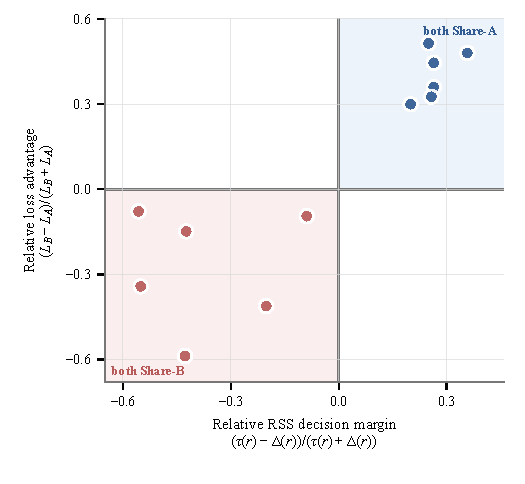
\includegraphics[width=\linewidth]{rss_relative_loss.pdf}
	    \caption{ Alignment Between RSS Decisions and Training-Loss Preference}
	    \label{fig:rss_training_loss_alignment}
	\end{figure}
	
	% \section{Experiment Details}
    \section*{Appendix E \\ Full Experiment Results}    
	\subsection*{Hyperparameters}
	Tables \ref{tab:lora_learning_rates} and \ref{tab:rslora_learning_rates} show the learning rates used for LoRA-based methods and rsLoRA-based methods, respectively. For the VeRA-based methods, we chose the AdamW optimizer and used separate learning rates for the classification head and the adapted layers as used in VeRA. The learning rates used for VeRA-based methods are shown in Table \ref{tab:vera_learning_rates}.
	\begin{table}[b]
		\centering
		\scriptsize
		\setlength{\tabcolsep}{1.5pt}
		\renewcommand{\arraystretch}{1.08}
		\begin{tabular*}{0.98\columnwidth}{@{\extracolsep{\fill}}lcccccc@{}}
			\toprule
			Method & MNLI-m & MNLI-mm & SST-2 & QNLI & QQP & RTE \\
			\midrule
			LoRA
			& 1E-2 & 1E-2 & 2E-2 & 1E-2 & 1E-2 & 1E-2 \\
			
			FFA-LoRA
			& 5E-2 & 5E-2 & 5E-2 & 2E-2 & 5E-2 & 2E-2 \\
			
			FedDPA-LoRA
			& 1E-2 & 1E-2 & 1E-2 & 5E-2 & 5E-2 & 1E-2 \\
			
			FedSA-LoRA
			& 2E-2 & 2E-2 & 1E-2 & 5E-3 & 2E-2 & 1E-2 \\
			
			FedAS-LoRA
			& 2E-2 & 2E-2 & 1E-2 & 5E-3 & 2E-2 & 1E-2 \\
			\bottomrule
		\end{tabular*}
		\caption{Learning rates used for LoRA-based methods on the GLUE benchmark.}
		\label{tab:lora_learning_rates}
	\end{table}
	\begin{table}[h]
		\centering
		\small
		\setlength{\tabcolsep}{1.5pt}
		\renewcommand{\arraystretch}{1.08}
		\begin{tabular*}{0.98\columnwidth}{@{\extracolsep{\fill}}lcccccc@{}}
			\toprule
			Method & MNLI-m & MNLI-mm & SST-2 & QNLI & QQP & RTE \\
			\midrule
			rsLoRA
			& 5E-3 & 5E-3 & 1E-2 & 2E-3 & 5E-3 & 2E-3 \\
			
			FFA-rsLoRA
			& 2E-2 & 2E-2 & 2E-2 & 1E-2 & 2E-2 & 1E-2 \\
			
			FedDPA-rsLoRA
			& 5E-3 & 5E-3 & 1E-2 & 1E-3 & 5E-3 & 1E-2 \\
			
			FedSA-rsLoRA
			& 5E-3 & 5E-3 & 5E-3 & 1E-3 & 2E-3 & 2E-3 \\
			
			FedAS-rsLoRA
			& 5E-3 & 5E-3 & 5E-3 & 1E-3 & 2E-3 & 2E-3 \\
			\bottomrule
		\end{tabular*}
		\caption{Learning rates used for rsLoRA-based methods on the GLUE benchmark.}
		\label{tab:rslora_learning_rates}
	\end{table}
	\begin{table}[t]
		\centering
		\small
		\setlength{\tabcolsep}{1.0pt}
		\renewcommand{\arraystretch}{1.08}
		\begin{tabular*}{0.98\columnwidth}{@{\extracolsep{\fill}}llcccccc@{}}
			\toprule
			Method & Position & \shortstack{MNLI-\\m} & \shortstack{MNLI-\\mm} & SST-2 & QNLI & QQP & RTE \\
			\midrule
			
			\multirow{2}{*}{VeRA}
			& VeRA & 1E-2 & 1E-2 & 2E-2 & 2E-3 & 2E-3 & 1E-2 \\
			& Head & 6E-3 & 6E-3 & 2E-3 & 3E-4 & 3E-4 & 2E-4 \\
			\midrule
			
			\multirow{2}{*}{FFA-VeRA}
			& VeRA & 2E-2 & 2E-2 & 1E-2 & 1E-2 & 1E-2 & 1E-2 \\
			& Head & 2E-3 & 2E-3 & 6E-3 & 2E-4 & 6E-3 & 2E-4 \\
			\midrule
			
			\multirow{2}{*}{FedDPA-VeRA}
			& VeRA & 1E-2 & 1E-2 & 1E-2 & 2E-3 & 2E-2 & 1E-2 \\
			& Head & 6E-3 & 6E-3 & 6E-3 & 3E-4 & 2E-3 & 2E-4 \\
			\midrule
			
			\multirow{2}{*}{FedSA-VeRA}
			& VeRA & 2E-3 & 2E-3 & 1E-2 & 1E-2 & 2E-3 & 1E-2 \\
			& Head & 3E-5 & 3E-5 & 3E-4 & 3E-4 & 3E-4 & 1E-4 \\
			\midrule
			
			\multirow{2}{*}{FedAS-VeRA}
			& VeRA & 2E-3 & 2E-3 & 1E-2 & 1E-2 & 2E-3 & 1E-2 \\
			& Head & 3E-5 & 3E-5 & 3E-4 & 3E-4 & 3E-4 & 1E-4 \\
			\bottomrule
		\end{tabular*}
		\caption{Learning rates used for VeRA-based methods on the GLUE benchmark.}
		\label{tab:vera_learning_rates}
	\end{table}
	
	\subsection*{Evaluation of RSS-Based Sharing-Side Selection}
	
	{\color{black}\paragraph{Alignment with Test-Accuracy Preference.}Table~\ref{tab:rss_metric_vs_share_acc_tau_gen} provides the full comparison between the sharing-side decisions made by RSS and the empirical test accuracies of Share-A/Local-B and Share-B/Local-A. The experiments cover six evaluation sets, multiple client partitions, and LoRA ranks $r\in\{2,4,8,16\}$. For each setting, RSS is computed before federated training, while the empirical winner is determined by comparing the test accuracies obtained at the best validation rounds of the two sharing strategies.
		
		Across the 38 evaluated settings, the RSS decision agrees with the empirically better sharing strategy in all 33 cases with a strict accuracy difference. The remaining five cases are marked as empirical ties in Table~\ref{tab:rss_metric_vs_share_acc_tau_gen}. The preferred sharing side also changes with the data partition and LoRA rank. For example, QNLI and MNLI favor Share-A/Local-B under the evaluated IID settings, whereas Share-B/Local-A is preferred in most of their Dirichlet settings. For MNLI under Dirichlet $\alpha=1$, the preferred strategy further changes from Share-B/Local-A at $r=4$ to Share-A/Local-B at $r=8$. Similarly, SST-2 favors Share-A/Local-B under IID partitions but mainly favors Share-B/Local-A under the non-IID partitions. These results support the use of a partition- and rank-aware selection rule instead of a fixed sharing policy. RSS should nevertheless be interpreted as a sharing-side selector rather than an estimator of the final accuracy gap between the two strategies.}

        {\color{black}\paragraph{Alignment with the training objective.}
Table~\ref{tab:rss_metric_vs_share_acc_tau_gen} compares the RSS
decision with the final test-accuracy preference of the two
fixed sharing strategies. We further examine whether the
decision direction of RSS agrees with their relative behavior
under the actual training objective. For visual illustration,
we randomly sample several evaluated settings and compare
their RSS decision margins with the corresponding training
losses of Share-A/Local-B and Share-B/Local-A.

For rank $r$, we define the relative RSS decision margin as
\begin{align}
    m_{\mathrm{RSS}}(r)
    =
    \frac{
        \tau(r)-\Delta(r)
    }{
        \tau(r)+\Delta(r)
    }.
    \label{eq:rss_relative_margin}
\end{align}
Since RSS selects Share-A/Local-B when
$\Delta(r)\leq\tau(r)$, a positive
$m_{\mathrm{RSS}}(r)$ favors Share-A/Local-B, whereas a
negative value favors Share-B/Local-A. We also define the
relative training-loss advantage as
\begin{align}
    m_{\mathrm{loss}}
    =
    \frac{
        L_B-L_A
    }{
        L_B+L_A
    },
    \label{eq:loss_relative_margin}
\end{align}
where $L_A$ and $L_B$ denote the training losses obtained
by Share-A/Local-B and Share-B/Local-A, respectively.
Accordingly, $m_{\mathrm{loss}}>0$ means that
Share-A/Local-B attains a lower training loss, while
$m_{\mathrm{loss}}<0$ means that Share-B/Local-A attains
a lower training loss.

As shown in Fig.~\ref{fig:rss_training_loss_alignment}, all
sampled cases lie in either the upper-right or lower-left
quadrant. Thus, the sharing side selected by RSS also attains
the lower training loss in these cases. This result provides
additional evidence that the RSS decision is consistent with
the optimization behavior of the two sharing strategies under
the actual task objective.

This directional agreement provides empirical support for
the residual-based selection principle in Theorem~1. The
theorem shows that the preferred sharing side is determined
by which shared-subspace constraint yields the smaller
aggregate projection residual. RSS translates this principle
into a training-free decision rule by assessing whether the
common rank-$r$ input-side subspace required by
Share-A/Local-B is sufficient for the client representations.
When this subspace is sufficient, RSS favors
Share-A/Local-B; otherwise, it favors Share-B/Local-A.
The consistent training-loss preference therefore indicates
that RSS identifies the sharing constraint that better fits the
client data under the actual task objective. This result
supports RSS as a practical proxy for the residual-based
sharing-side preference characterized in Theorem~\ref{tab:rss_metric_vs_share_acc_tau_gen}.}
	% \begin{table}[H]
		%     \centering
		%     \caption{Comparison of RSS metric decisions with empirical Share-A/Local-B and Share-B/Local-A test accuracy under three-client settings.}
		%     \label{tab:sass_metric_vs_share_acc}
		%     \scriptsize
		%     \setlength{\tabcolsep}{2.5pt}
		%     \renewcommand{\arraystretch}{1.08}
		%     \resizebox{\columnwidth}{!}{%
			%     \begin{tabular}{@{}llccccccccc@{}}
				%         \toprule
				%         \multirow{2}{*}{Dataset}
				%         & \multirow{2}{*}{Split}
				%         & \multirow{2}{*}{$r$}
				%         & \multicolumn{4}{c}{RSS metric}
				%         & \multicolumn{3}{c}{Empirical accuracy (\%)}
				%         & \multirow{2}{*}{Alignment} \\
				%         \cmidrule(lr){4-7}\cmidrule(lr){8-10}
				%         & & & RSS$(r)$ & $\Delta_{\mathrm{obs}}$ & $\tau_{\mathrm{gen}}$
				%         & Decision & Share-A & Share-B & Winner & \\
				%         \midrule
				%         \multirow{8}{*}{\textbf{QNLI}} & \multirow{2}{*}{IID} & 4 & 0.9999754 & $2.46413\!\times\!10^{-5}$ & $3.91172\!\times\!10^{-5}$ & Share-A & 61.93 & \textbf{73.13} & \textbf{Share-B}\textsuperscript{$\dagger$} & \cellcolor{red!15}\textcolor{red!70!black}{\textbf{Mismatch}} \\
				%          &  & 8 & 0.9999572 & $4.28222\!\times\!10^{-5}$ & $7.07299\!\times\!10^{-5}$ & Share-A & 80.01 & \textbf{92.02} & \textbf{Share-B}\textsuperscript{$\dagger$} & \cellcolor{red!15}\textcolor{red!70!black}{\textbf{Mismatch}} \\
				%                 \cmidrule(lr){2-11}
				%          & \multirow{4}{*}{Dirichlet $\alpha=0.5$} & 2 & 0.9999698 & $3.01960\!\times\!10^{-5}$ & $3.46345\!\times\!10^{-5}$ & Share-A & \textbf{72.46} & 71.84 & \textbf{Share-A} & \cellcolor{green!12}\textcolor{green!40!black}{Match} \\
				%          &  & 4 & 0.9999411 & $5.89316\!\times\!10^{-5}$ & $3.80830\!\times\!10^{-5}$ & Share-B & \textbf{64.77} & 63.93 & \textbf{Share-A} & \cellcolor{red!15}\textcolor{red!70!black}{\textbf{Mismatch}} \\
				%          &  & 8 & 0.9999263 & $7.37366\!\times\!10^{-5}$ & $6.79052\!\times\!10^{-5}$ & Share-B & \textbf{91.10} & 77.41 & \textbf{Share-A} & \cellcolor{red!15}\textcolor{red!70!black}{\textbf{Mismatch}} \\
				%          &  & 16 & 0.9998661 & $1.33945\!\times\!10^{-4}$ & $1.31365\!\times\!10^{-4}$ & Uncertain & 67.12 & \textbf{89.56} & \textbf{Share-B} & \cellcolor{yellow!25}{Metric uncertain} \\
				%                 \cmidrule(lr){2-11}
				%          & \multirow{2}{*}{Dirichlet $\alpha=1$} & 4 & 0.9999409 & $5.90747\!\times\!10^{-5}$ & $3.92434\!\times\!10^{-5}$ & Share-B & \textbf{73.21} & 73.10 & \textbf{Share-A}\textsuperscript{$\dagger$} & \cellcolor{red!15}\textcolor{red!70!black}{\textbf{Mismatch}} \\
				%          &  & 8 & 0.9999168 & $8.31570\!\times\!10^{-5}$ & $6.96169\!\times\!10^{-5}$ & Share-B & 74.89 & \textbf{85.58} & \textbf{Share-B} & \cellcolor{green!12}\textcolor{green!40!black}{Match} \\
				%                 \midrule
				%         \multirow{2}{*}{\textbf{QQP}\textsuperscript{$\ddagger$}} & \multirow{2}{*}{Dirichlet $\alpha=0.5$} & 4 & 0.9999788 & $2.11905\!\times\!10^{-5}$ & $1.28376\!\times\!10^{-5}$ & Share-B & \textbf{86.73} & 81.71 & \textbf{Share-A} & \cellcolor{red!15}\textcolor{red!70!black}{\textbf{Mismatch}} \\
				%          &  & 8 & 0.9999585 & $4.14507\!\times\!10^{-5}$ & $1.67622\!\times\!10^{-5}$ & Share-B & \textbf{85.65} & 78.13 & \textbf{Share-A} & \cellcolor{red!15}\textcolor{red!70!black}{\textbf{Mismatch}} \\
				%                 \midrule
				%         \multirow{8}{*}{\textbf{SST-2}} & \multirow{2}{*}{IID} & 4 & 0.9996108 & $3.89196\!\times\!10^{-4}$ & $5.07871\!\times\!10^{-4}$ & Share-A & 95.41 & \textbf{96.56} & \textbf{Share-B}\textsuperscript{$\dagger$} & \cellcolor{red!15}\textcolor{red!70!black}{\textbf{Mismatch}} \\
				%          &  & 8 & 0.9995641 & $4.35904\!\times\!10^{-4}$ & $6.02930\!\times\!10^{-4}$ & Share-A & 94.72 & \textbf{96.10} & \textbf{Share-B}\textsuperscript{$\dagger$} & \cellcolor{red!15}\textcolor{red!70!black}{\textbf{Mismatch}} \\
				%                 \cmidrule(lr){2-11}
				%          & \multirow{4}{*}{Dirichlet $\alpha=0.5$} & 2 & 0.9985460 & $1.45398\!\times\!10^{-3}$ & $5.83336\!\times\!10^{-4}$ & Share-B & 96.56 & \textbf{96.79} & \textbf{Share-B} & \cellcolor{green!12}\textcolor{green!40!black}{Match} \\
				%          &  & 4 & 0.9981555 & $1.84450\!\times\!10^{-3}$ & $5.25775\!\times\!10^{-4}$ & Share-B & \textbf{96.33} & \textbf{96.33} & \textbf{Tie} & \cellcolor{yellow!25}{Actual tie} \\
				%          &  & 8 & 0.9977975 & $2.20251\!\times\!10^{-3}$ & $6.38468\!\times\!10^{-4}$ & Share-B & \textbf{96.56} & 95.64 & \textbf{Share-A} & \cellcolor{red!15}\textcolor{red!70!black}{\textbf{Mismatch}} \\
				%          &  & 16 & 0.9963678 & $3.63222\!\times\!10^{-3}$ & $1.01451\!\times\!10^{-3}$ & Share-B & \textbf{95.64} & 94.72 & \textbf{Share-A} & \cellcolor{red!15}\textcolor{red!70!black}{\textbf{Mismatch}} \\
				%                 \cmidrule(lr){2-11}
				%          & \multirow{2}{*}{Dirichlet $\alpha=1$} & 4 & 0.9988155 & $1.18446\!\times\!10^{-3}$ & $5.79445\!\times\!10^{-4}$ & Share-B & \textbf{97.02} & \textbf{97.02} & \textbf{Tie} & \cellcolor{yellow!25}{Actual tie} \\
				%          &  & 8 & 0.9985669 & $1.43308\!\times\!10^{-3}$ & $6.62178\!\times\!10^{-4}$ & Share-B & 96.56 & \textbf{96.79} & \textbf{Share-B} & \cellcolor{green!12}\textcolor{green!40!black}{Match} \\
				%                 \midrule
				%         \multirow{8}{*}{\textbf{MNLI-m}} & \multirow{2}{*}{IID} & 4 & 0.9999940 & $5.98420\!\times\!10^{-6}$ & $1.02906\!\times\!10^{-5}$ & Share-A & \textbf{87.06} & 63.11 & \textbf{Share-A} & \cellcolor{green!12}\textcolor{green!40!black}{Match} \\
				%          &  & 8 & 0.9999708 & $2.91890\!\times\!10^{-5}$ & $4.13822\!\times\!10^{-5}$ & Share-A & 86.49 & \textbf{87.39} & \textbf{Share-B} & \cellcolor{red!15}\textcolor{red!70!black}{\textbf{Mismatch}} \\
				%                 \cmidrule(lr){2-11}
				%          & \multirow{4}{*}{Dirichlet $\alpha=0.5$} & 2 & 0.9998969 & $1.03136\!\times\!10^{-4}$ & $1.11881\!\times\!10^{-5}$ & Share-B & \textbf{89.79} & 88.87 & \textbf{Share-A} & \cellcolor{red!15}\textcolor{red!70!black}{\textbf{Mismatch}} \\
				%          &  & 4 & 0.9999538 & $4.62360\!\times\!10^{-5}$ & $9.96230\!\times\!10^{-6}$ & Share-B & 90.01 & \textbf{90.28} & \textbf{Share-B} & \cellcolor{green!12}\textcolor{green!40!black}{Match} \\
				%          &  & 8 & 0.9999067 & $9.33286\!\times\!10^{-5}$ & $3.98546\!\times\!10^{-5}$ & Share-B & 89.77 & \textbf{89.95} & \textbf{Share-B} & \cellcolor{green!12}\textcolor{green!40!black}{Match} \\
				%          &  & 16 & 0.9999192 & $8.07826\!\times\!10^{-5}$ & $3.45278\!\times\!10^{-5}$ & Share-B & \textbf{88.75} & 88.73 & \textbf{Share-A} & \cellcolor{red!15}\textcolor{red!70!black}{\textbf{Mismatch}} \\
				%                 \cmidrule(lr){2-11}
				%          & \multirow{2}{*}{Dirichlet $\alpha=1$} & 4 & 0.9999862 & $1.37597\!\times\!10^{-5}$ & $1.02455\!\times\!10^{-5}$ & Share-B & 64.51 & \textbf{64.62} & \textbf{Share-B} & \cellcolor{green!12}\textcolor{green!40!black}{Match} \\
				%          &  & 8 & 0.9999674 & $3.26219\!\times\!10^{-5}$ & $3.80408\!\times\!10^{-5}$ & Share-A & 90.41 & \textbf{90.57} & \textbf{Share-B} & \cellcolor{red!15}\textcolor{red!70!black}{\textbf{Mismatch}} \\
				%                 \midrule
				%         \multirow{6}{*}{\textbf{MNLI-mm}} & \multirow{2}{*}{IID} & 4 & 0.9999940 & $5.98420\!\times\!10^{-6}$ & $1.02906\!\times\!10^{-5}$ & Share-A & \textbf{86.68} & 85.23 & \textbf{Share-A} & \cellcolor{green!12}\textcolor{green!40!black}{Match} \\
				%          &  & 8 & 0.9999708 & $2.91890\!\times\!10^{-5}$ & $4.13822\!\times\!10^{-5}$ & Share-A & 85.84 & \textbf{86.35} & \textbf{Share-B} & \cellcolor{red!15}\textcolor{red!70!black}{\textbf{Mismatch}} \\
				%                 \cmidrule(lr){2-11}
				%          & \multirow{2}{*}{Dirichlet $\alpha=0.5$} & 4 & 0.9999538 & $4.62360\!\times\!10^{-5}$ & $9.96230\!\times\!10^{-6}$ & Share-B & \textbf{90.50} & 88.38 & \textbf{Share-A} & \cellcolor{red!15}\textcolor{red!70!black}{\textbf{Mismatch}} \\
				%          &  & 8 & 0.9999067 & $9.33286\!\times\!10^{-5}$ & $3.98546\!\times\!10^{-5}$ & Share-B & 90.80 & \textbf{90.86} & \textbf{Share-B} & \cellcolor{green!12}\textcolor{green!40!black}{Match} \\
				%                 \cmidrule(lr){2-11}
				%          & \multirow{2}{*}{Dirichlet $\alpha=1$} & 4 & 0.9999862 & $1.37597\!\times\!10^{-5}$ & $1.02455\!\times\!10^{-5}$ & Share-B & 66.16 & \textbf{88.79} & \textbf{Share-B} & \cellcolor{green!12}\textcolor{green!40!black}{Match} \\
				%          &  & 8 & 0.9999674 & $3.26219\!\times\!10^{-5}$ & $3.80408\!\times\!10^{-5}$ & Share-A & \textbf{90.44} & 77.97 & \textbf{Share-A} & \cellcolor{green!12}\textcolor{green!40!black}{Match} \\
				%                 \midrule
				%         \multirow{6}{*}{\textbf{RTE}} & \multirow{2}{*}{IID} & 4 & 0.9979225 & $2.07749\!\times\!10^{-3}$ & $3.52261\!\times\!10^{-3}$ & Share-A & 77.70 & \textbf{79.14} & \textbf{Share-B}\textsuperscript{$\dagger$} & \cellcolor{red!15}\textcolor{red!70!black}{\textbf{Mismatch}} \\
				%          &  & 8 & 0.9960091 & $3.99091\!\times\!10^{-3}$ & $5.98761\!\times\!10^{-3}$ & Share-A & 76.98 & \textbf{79.86} & \textbf{Share-B}\textsuperscript{$\dagger$} & \cellcolor{red!15}\textcolor{red!70!black}{\textbf{Mismatch}} \\
				%                 \cmidrule(lr){2-11}
				%          & \multirow{2}{*}{Dirichlet $\alpha=0.5$} & 4 & 0.9981881 & $1.81187\!\times\!10^{-3}$ & $3.83366\!\times\!10^{-3}$ & Share-A & \textbf{79.71} & \textbf{79.71} & \textbf{Tie} & \cellcolor{yellow!25}{Actual tie} \\
				%          &  & 8 & 0.9963619 & $3.63808\!\times\!10^{-3}$ & $5.98369\!\times\!10^{-3}$ & Share-A & \textbf{87.77} & \textbf{87.77} & \textbf{Tie} & \cellcolor{yellow!25}{Actual tie} \\
				%                 \cmidrule(lr){2-11}
				%          & \multirow{2}{*}{Dirichlet $\alpha=1$} & 4 & 0.9981738 & $1.82618\!\times\!10^{-3}$ & $3.55810\!\times\!10^{-3}$ & Share-A & \textbf{66.19} & 65.47 & \textbf{Share-A} & \cellcolor{green!12}\textcolor{green!40!black}{Match} \\
				%          &  & 8 & 0.9965479 & $3.45208\!\times\!10^{-3}$ & $5.75546\!\times\!10^{-3}$ & Share-A & \textbf{76.26} & 68.35 & \textbf{Share-A} & \cellcolor{green!12}\textcolor{green!40!black}{Match} \\
				%         \bottomrule
				%     \end{tabular}%
			%     }
		
		%     \vspace{1mm}
		%     \parbox{\columnwidth}{\scriptsize
			%     \emph{Note:} Accuracy values are percentages; the higher value is bold. Winners are determined from the unrounded accuracies. Red cells denote a directional mismatch between the RSS decision and the empirical winner; yellow cells denote an empirical tie or an uncertain metric decision. All rows use standard LoRA, full participation (3/3 clients), and seed 42. MNLI-m and MNLI-mm share the same task-level MNLI RSS metric but retain separate empirical accuracies. Rows marked $\dagger$ are flagged as \textit{Needs rerun} in the source workbook and are reported as the current available results. For QQP, $\ddagger$ denotes nominal split alignment: the RSS artifact used deterministic Dirichlet $\alpha=0.5$ reconstruction, while the training artifacts contain no partition hash for sample-level matching.}
		% \end{table}
	
	% \begin{table}[H]
		%     \centering
		%     \caption{Comparison of RSS metric decisions using the binary $\tau_{\mathrm{gen}}$ rule with empirical Share-A/Local-B and Share-B/Local-A test accuracy under three-client settings.}
		%     \label{tab:rss_metric_vs_share_acc_tau_gen}
		%     \scriptsize
		%     \setlength{\tabcolsep}{2.5pt}
		%     \renewcommand{\arraystretch}{1.08}
		%     \resizebox{\columnwidth}{!}{%
			%     \begin{tabular}{@{}llccccccccc@{}}
				%         \toprule
				%         \multirow{2}{*}{Dataset}
				%         & \multirow{2}{*}{Split}
				%         & \multirow{2}{*}{$r$}
				%         & \multicolumn{4}{c}{RSS metric}
				%         & \multicolumn{3}{c}{Empirical accuracy (\%)}
				%         & \multirow{2}{*}{Alignment} \\
				%         \cmidrule(lr){4-7}\cmidrule(lr){8-10}
				%         & & & RSS$(r)$ & $\Delta_{\mathrm{obs}}$ & $\tau_{\mathrm{gen}}$
				%         & Decision & Share-A & Share-B & Winner & \\
				%         \midrule
				%         \multirow{8}{*}{\textbf{QNLI}} & \multirow{2}{*}{IID} & 4 & 0.9999754 & $2.46413\!\times\!10^{-5}$ & $3.91172\!\times\!10^{-5}$ & Share-A & 61.93 & \textbf{73.13} & \textbf{Share-B}\textsuperscript{$\dagger$} & \cellcolor{red!15}\textcolor{red!70!black}{\textbf{Mismatch}} \\
				%          &  & 8 & 0.9999572 & $4.28222\!\times\!10^{-5}$ & $7.07299\!\times\!10^{-5}$ & Share-A & 80.01 & \textbf{92.02} & \textbf{Share-B}\textsuperscript{$\dagger$} & \cellcolor{red!15}\textcolor{red!70!black}{\textbf{Mismatch}} \\
				%                 \cmidrule(lr){2-11}
				%          & \multirow{4}{*}{Dirichlet $\alpha=0.5$} & 2 & 0.9999698 & $3.01960\!\times\!10^{-5}$ & $3.46345\!\times\!10^{-5}$ & Share-A & \textbf{72.46} & 71.84 & \textbf{Share-A} & \cellcolor{green!12}\textcolor{green!40!black}{Match} \\
				%          &  & 4 & 0.9999411 & $5.89316\!\times\!10^{-5}$ & $3.80830\!\times\!10^{-5}$ & Share-B & \textbf{64.77} & 63.93 & \textbf{Share-A} & \cellcolor{red!15}\textcolor{red!70!black}{\textbf{Mismatch}} \\
				%          &  & 8 & 0.9999263 & $7.37366\!\times\!10^{-5}$ & $6.79052\!\times\!10^{-5}$ & Share-B & \textbf{91.10} & 77.41 & \textbf{Share-A} & \cellcolor{red!15}\textcolor{red!70!black}{\textbf{Mismatch}} \\
				%          &  & 16 & 0.9998661 & $1.33945\!\times\!10^{-4}$ & $1.31365\!\times\!10^{-4}$ & Share-B & 67.12 & \textbf{89.56} & \textbf{Share-B} & \cellcolor{green!12}\textcolor{green!40!black}{Match} \\
				%                 \cmidrule(lr){2-11}
				%          & \multirow{2}{*}{Dirichlet $\alpha=1$} & 4 & 0.9999409 & $5.90747\!\times\!10^{-5}$ & $3.92434\!\times\!10^{-5}$ & Share-B & \textbf{73.21} & 73.10 & \textbf{Share-A}\textsuperscript{$\dagger$} & \cellcolor{red!15}\textcolor{red!70!black}{\textbf{Mismatch}} \\
				%          &  & 8 & 0.9999168 & $8.31570\!\times\!10^{-5}$ & $6.96169\!\times\!10^{-5}$ & Share-B & 74.89 & \textbf{85.58} & \textbf{Share-B} & \cellcolor{green!12}\textcolor{green!40!black}{Match} \\
				%                 \midrule
				%         \multirow{2}{*}{\textbf{QQP}\textsuperscript{$\ddagger$}} & \multirow{2}{*}{Dirichlet $\alpha=0.5$} & 4 & 0.9999788 & $2.11905\!\times\!10^{-5}$ & $1.28376\!\times\!10^{-5}$ & Share-B & \textbf{86.73} & 81.71 & \textbf{Share-A} & \cellcolor{red!15}\textcolor{red!70!black}{\textbf{Mismatch}} \\
				%          &  & 8 & 0.9999585 & $4.14507\!\times\!10^{-5}$ & $1.67622\!\times\!10^{-5}$ & Share-B & \textbf{85.65} & 78.13 & \textbf{Share-A} & \cellcolor{red!15}\textcolor{red!70!black}{\textbf{Mismatch}} \\
				%                 \midrule
				%         \multirow{8}{*}{\textbf{SST-2}} & \multirow{2}{*}{IID} & 4 & 0.9996108 & $3.89196\!\times\!10^{-4}$ & $5.07871\!\times\!10^{-4}$ & Share-A & 95.41 & \textbf{96.56} & \textbf{Share-B}\textsuperscript{$\dagger$} & \cellcolor{red!15}\textcolor{red!70!black}{\textbf{Mismatch}} \\
				%          &  & 8 & 0.9995641 & $4.35904\!\times\!10^{-4}$ & $6.02930\!\times\!10^{-4}$ & Share-A & 94.72 & \textbf{96.10} & \textbf{Share-B}\textsuperscript{$\dagger$} & \cellcolor{red!15}\textcolor{red!70!black}{\textbf{Mismatch}} \\
				%                 \cmidrule(lr){2-11}
				%          & \multirow{4}{*}{Dirichlet $\alpha=0.5$} & 2 & 0.9985460 & $1.45398\!\times\!10^{-3}$ & $5.83336\!\times\!10^{-4}$ & Share-B & 96.56 & \textbf{96.79} & \textbf{Share-B} & \cellcolor{green!12}\textcolor{green!40!black}{Match} \\
				%          &  & 4 & 0.9981555 & $1.84450\!\times\!10^{-3}$ & $5.25775\!\times\!10^{-4}$ & Share-B & \textbf{96.33} & \textbf{96.33} & \textbf{Tie} & \cellcolor{yellow!25}{Actual tie} \\
				%          &  & 8 & 0.9977975 & $2.20251\!\times\!10^{-3}$ & $6.38468\!\times\!10^{-4}$ & Share-B & \textbf{96.56} & 95.64 & \textbf{Share-A} & \cellcolor{red!15}\textcolor{red!70!black}{\textbf{Mismatch}} \\
				%          &  & 16 & 0.9963678 & $3.63222\!\times\!10^{-3}$ & $1.01451\!\times\!10^{-3}$ & Share-B & \textbf{95.64} & 94.72 & \textbf{Share-A} & \cellcolor{red!15}\textcolor{red!70!black}{\textbf{Mismatch}} \\
				%                 \cmidrule(lr){2-11}
				%          & \multirow{2}{*}{Dirichlet $\alpha=1$} & 4 & 0.9988155 & $1.18446\!\times\!10^{-3}$ & $5.79445\!\times\!10^{-4}$ & Share-B & \textbf{97.02} & \textbf{97.02} & \textbf{Tie} & \cellcolor{yellow!25}{Actual tie} \\
				%          &  & 8 & 0.9985669 & $1.43308\!\times\!10^{-3}$ & $6.62178\!\times\!10^{-4}$ & Share-B & 96.56 & \textbf{96.79} & \textbf{Share-B} & \cellcolor{green!12}\textcolor{green!40!black}{Match} \\
				%                 \midrule
				%         \multirow{8}{*}{\textbf{MNLI-m}} & \multirow{2}{*}{IID} & 4 & 0.9999940 & $5.98420\!\times\!10^{-6}$ & $1.02906\!\times\!10^{-5}$ & Share-A & \textbf{87.06} & 63.11 & \textbf{Share-A} & \cellcolor{green!12}\textcolor{green!40!black}{Match} \\
				%          &  & 8 & 0.9999708 & $2.91890\!\times\!10^{-5}$ & $4.13822\!\times\!10^{-5}$ & Share-A & 86.49 & \textbf{87.39} & \textbf{Share-B} & \cellcolor{red!15}\textcolor{red!70!black}{\textbf{Mismatch}} \\
				%                 \cmidrule(lr){2-11}
				%          & \multirow{4}{*}{Dirichlet $\alpha=0.5$} & 2 & 0.9998969 & $1.03136\!\times\!10^{-4}$ & $1.11881\!\times\!10^{-5}$ & Share-B & \textbf{89.79} & 88.87 & \textbf{Share-A} & \cellcolor{red!15}\textcolor{red!70!black}{\textbf{Mismatch}} \\
				%          &  & 4 & 0.9999538 & $4.62360\!\times\!10^{-5}$ & $9.96230\!\times\!10^{-6}$ & Share-B & 90.01 & \textbf{90.28} & \textbf{Share-B} & \cellcolor{green!12}\textcolor{green!40!black}{Match} \\
				%          &  & 8 & 0.9999067 & $9.33286\!\times\!10^{-5}$ & $3.98546\!\times\!10^{-5}$ & Share-B & 89.77 & \textbf{89.95} & \textbf{Share-B} & \cellcolor{green!12}\textcolor{green!40!black}{Match} \\
				%          &  & 16 & 0.9999192 & $8.07826\!\times\!10^{-5}$ & $3.45278\!\times\!10^{-5}$ & Share-B & \textbf{88.75} & 88.73 & \textbf{Share-A} & \cellcolor{red!15}\textcolor{red!70!black}{\textbf{Mismatch}} \\
				%                 \cmidrule(lr){2-11}
				%          & \multirow{2}{*}{Dirichlet $\alpha=1$} & 4 & 0.9999862 & $1.37597\!\times\!10^{-5}$ & $1.02455\!\times\!10^{-5}$ & Share-B & 64.51 & \textbf{64.62} & \textbf{Share-B} & \cellcolor{green!12}\textcolor{green!40!black}{Match} \\
				%          &  & 8 & 0.9999674 & $3.26219\!\times\!10^{-5}$ & $3.80408\!\times\!10^{-5}$ & Share-A & 90.41 & \textbf{90.57} & \textbf{Share-B} & \cellcolor{red!15}\textcolor{red!70!black}{\textbf{Mismatch}} \\
				%                 \midrule
				%         \multirow{6}{*}{\textbf{MNLI-mm}} & \multirow{2}{*}{IID} & 4 & 0.9999940 & $5.98420\!\times\!10^{-6}$ & $1.02906\!\times\!10^{-5}$ & Share-A & \textbf{86.68} & 85.23 & \textbf{Share-A} & \cellcolor{green!12}\textcolor{green!40!black}{Match} \\
				%          &  & 8 & 0.9999708 & $2.91890\!\times\!10^{-5}$ & $4.13822\!\times\!10^{-5}$ & Share-A & 85.84 & \textbf{86.35} & \textbf{Share-B} & \cellcolor{red!15}\textcolor{red!70!black}{\textbf{Mismatch}} \\
				%                 \cmidrule(lr){2-11}
				%          & \multirow{2}{*}{Dirichlet $\alpha=0.5$} & 4 & 0.9999538 & $4.62360\!\times\!10^{-5}$ & $9.96230\!\times\!10^{-6}$ & Share-B & \textbf{90.50} & 88.38 & \textbf{Share-A} & \cellcolor{red!15}\textcolor{red!70!black}{\textbf{Mismatch}} \\
				%          &  & 8 & 0.9999067 & $9.33286\!\times\!10^{-5}$ & $3.98546\!\times\!10^{-5}$ & Share-B & 90.80 & \textbf{90.86} & \textbf{Share-B} & \cellcolor{green!12}\textcolor{green!40!black}{Match} \\
				%                 \cmidrule(lr){2-11}
				%          & \multirow{2}{*}{Dirichlet $\alpha=1$} & 4 & 0.9999862 & $1.37597\!\times\!10^{-5}$ & $1.02455\!\times\!10^{-5}$ & Share-B & 66.16 & \textbf{88.79} & \textbf{Share-B} & \cellcolor{green!12}\textcolor{green!40!black}{Match} \\
				%          &  & 8 & 0.9999674 & $3.26219\!\times\!10^{-5}$ & $3.80408\!\times\!10^{-5}$ & Share-A & \textbf{90.44} & 77.97 & \textbf{Share-A} & \cellcolor{green!12}\textcolor{green!40!black}{Match} \\
				%                 \midrule
				%         \multirow{6}{*}{\textbf{RTE}} & \multirow{2}{*}{IID} & 4 & 0.9979225 & $2.07749\!\times\!10^{-3}$ & $3.52261\!\times\!10^{-3}$ & Share-A & 77.70 & \textbf{79.14} & \textbf{Share-B}\textsuperscript{$\dagger$} & \cellcolor{red!15}\textcolor{red!70!black}{\textbf{Mismatch}} \\
				%          &  & 8 & 0.9960091 & $3.99091\!\times\!10^{-3}$ & $5.98761\!\times\!10^{-3}$ & Share-A & 76.98 & \textbf{79.86} & \textbf{Share-B}\textsuperscript{$\dagger$} & \cellcolor{red!15}\textcolor{red!70!black}{\textbf{Mismatch}} \\
				%                 \cmidrule(lr){2-11}
				%          & \multirow{2}{*}{Dirichlet $\alpha=0.5$} & 4 & 0.9981881 & $1.81187\!\times\!10^{-3}$ & $3.83366\!\times\!10^{-3}$ & Share-A & \textbf{79.71} & \textbf{79.71} & \textbf{Tie} & \cellcolor{yellow!25}{Actual tie} \\
				%          &  & 8 & 0.9963619 & $3.63808\!\times\!10^{-3}$ & $5.98369\!\times\!10^{-3}$ & Share-A & \textbf{87.77} & \textbf{87.77} & \textbf{Tie} & \cellcolor{yellow!25}{Actual tie} \\
				%                 \cmidrule(lr){2-11}
				%          & \multirow{2}{*}{Dirichlet $\alpha=1$} & 4 & 0.9981738 & $1.82618\!\times\!10^{-3}$ & $3.55810\!\times\!10^{-3}$ & Share-A & \textbf{66.19} & 65.47 & \textbf{Share-A} & \cellcolor{green!12}\textcolor{green!40!black}{Match} \\
				%          &  & 8 & 0.9965479 & $3.45208\!\times\!10^{-3}$ & $5.75546\!\times\!10^{-3}$ & Share-A & \textbf{76.26} & 68.35 & \textbf{Share-A} & \cellcolor{green!12}\textcolor{green!40!black}{Match} \\
				%         \bottomrule
				%     \end{tabular}%
			%     }
		
		%     \vspace{1mm}
		%     \parbox{\columnwidth}{\scriptsize
			%     \emph{Note:} The decision follows the binary $\tau_{\mathrm{gen}}$ rule: Share-B/Local-A when $\Delta_{\mathrm{obs}}>\tau_{\mathrm{gen}}$, and Share-A/Local-B when $\Delta_{\mathrm{obs}}\leq\tau_{\mathrm{gen}}$. No $\tau_{\mathrm{high}}$, $\tau_{\mathrm{low}}$, uncertainty band, or \textit{Uncertain} category is used. Accuracy values are percentages; the higher value is bold, and winners are determined from the unrounded accuracies. Red cells denote a directional mismatch; yellow cells denote an empirical tie. All rows use standard LoRA, full participation (3/3 clients), and seed 42. MNLI-m and MNLI-mm share the same task-level MNLI RSS metric but retain separate empirical accuracies. Rows marked $\dagger$ are flagged as \textit{Needs rerun} in the source workbook and are reported as the current available results. For QQP, $\ddagger$ denotes nominal split alignment: the RSS artifact used deterministic Dirichlet $\alpha=0.5$ reconstruction, while the training artifacts contain no partition hash for sample-level matching.}
		% \end{table}
	
	\begin{table*}[!t]
		\centering
		\scriptsize
		\setlength{\tabcolsep}{2.5pt}
		\renewcommand{\arraystretch}{1.08}
		\resizebox{0.93\textwidth}{!}{%
			\begin{tabular}{@{}llcccccccc@{}}
				\toprule
				\multirow{2}{*}{Dataset}
				& \multirow{2}{*}{Split}
				& \multirow{2}{*}{$r$}
				& \multicolumn{3}{c}{RSS metric}
				& \multicolumn{3}{c}{Accuracy (\%)}
				& \multirow{2}{*}{Alignment} \\
				\cmidrule(lr){4-6}\cmidrule(lr){7-9}
				& & & $\Delta(r)$ & $\tau (r)$
				& Decision & Share-A & Share-B & Winner & \\
				\midrule
				\multirow{8}{*}{\textbf{QNLI}} & \multirow{2}{*}{IID} & 4 & $2.46413\!\times\!10^{-5}$ & $3.91172\!\times\!10^{-5}$ & Share-A & \textbf{92.26} & 90.18 & \textbf{Share-A} & Match \\
				&  & 8 & $4.28222\!\times\!10^{-5}$ & $7.07299\!\times\!10^{-5}$ & Share-A & \textbf{91.12} & 90.66 & \textbf{Share-A} & Match \\
				& \multirow{4}{*}{Dirichlet $\alpha=0.5$} & 2 & $3.01960\!\times\!10^{-5}$ & $3.46345\!\times\!10^{-5}$ & Share-A & \textbf{89.46} & 88.84 & \textbf{Share-A} & Match \\
				&  & 4 & $5.89316\!\times\!10^{-5}$ & $3.80830\!\times\!10^{-5}$ & Share-B & 92.01 & \textbf{92.80} & \textbf{Share-B} & Match \\
				&  & 8 & $7.37366\!\times\!10^{-5}$ & $6.79052\!\times\!10^{-5}$ & Share-B & 91.13 & \textbf{92.94} & \textbf{Share-B} & Match \\
				&  & 16 & $1.33945\!\times\!10^{-4}$ & $1.31365\!\times\!10^{-4}$ & Share-B & 89.12 & \textbf{89.56} & \textbf{Share-B} & Match \\
				& \multirow{2}{*}{Dirichlet $\alpha=1$} & 4 & $5.90747\!\times\!10^{-5}$ & $3.92434\!\times\!10^{-5}$ & Share-B & 93.28 & \textbf{94.69} & \textbf{Share-B} & Match \\
				&  & 8 & $8.31570\!\times\!10^{-5}$ & $6.96169\!\times\!10^{-5}$ & Share-B & 90.89 & \textbf{91.58} & \textbf{Share-B} & Match \\
				\midrule
				\multirow{2}{*}{\textbf{QQP}} & \multirow{2}{*}{Dirichlet $\alpha=0.5$} & 4 & $2.11905\!\times\!10^{-5}$ & $1.28376\!\times\!10^{-5}$ & Share-B & 85.68 & \textbf{86.70} & \textbf{Share-B} & Match \\
				&  & 8 & $4.14507\!\times\!10^{-5}$ & $1.67622\!\times\!10^{-5}$ & Share-B & 86.87 & \textbf{87.95} & \textbf{Share-B} & Match \\
				\midrule
				\multirow{8}{*}{\textbf{SST-2}} & \multirow{2}{*}{IID} & 4 & $3.89196\!\times\!10^{-4}$ & $5.07871\!\times\!10^{-4}$ & Share-A & \textbf{96.65} & 96.14 & \textbf{Share-A} & Match \\
				&  & 8 & $4.35904\!\times\!10^{-4}$ & $6.02930\!\times\!10^{-4}$ & Share-A & \textbf{96.10} & 95.87 & \textbf{Share-A} & Match \\
				& \multirow{4}{*}{Dirichlet $\alpha=0.5$} & 2 & $1.45398\!\times\!10^{-3}$ & $5.83336\!\times\!10^{-4}$ & Share-B & 96.56 & \textbf{96.79} & \textbf{Share-B} & Match \\
				&  & 4 & $1.84450\!\times\!10^{-3}$ & $5.25775\!\times\!10^{-4}$ & Share-B & \textbf{96.33} & \textbf{96.33} & \textbf{Tie} & Actual tie \\
				&  & 8 & $2.20251\!\times\!10^{-3}$ & $6.38468\!\times\!10^{-4}$ & Share-B & 95.72 & \textbf{97.17} & \textbf{Share-B} & Match \\
				&  & 16 & $3.63222\!\times\!10^{-3}$ & $1.01451\!\times\!10^{-3}$ & Share-B & \textbf{95.73} & 95.72 & \textbf{Tie} & Actual tie \\
				& \multirow{2}{*}{Dirichlet $\alpha=1$} & 4 & $1.18446\!\times\!10^{-3}$ & $5.79445\!\times\!10^{-4}$ & Share-B & \textbf{97.02} & \textbf{97.02} & \textbf{Tie} & Actual tie \\
				&  & 8 & $1.43308\!\times\!10^{-3}$ & $6.62178\!\times\!10^{-4}$ & Share-B & 96.56 & \textbf{96.79} & \textbf{Share-B} & Match \\
				\midrule
				\multirow{8}{*}{\textbf{MNLI-m}} & \multirow{2}{*}{IID} & 4 & $5.98420\!\times\!10^{-6}$ & $1.02906\!\times\!10^{-5}$ & Share-A & \textbf{87.06} & 86.11 & \textbf{Share-A} & Match \\
				&  & 8 & $2.91890\!\times\!10^{-5}$ & $4.13822\!\times\!10^{-5}$ & Share-A & \textbf{89.43} & 89.06 & \textbf{Share-A} & Match \\
				& \multirow{4}{*}{Dirichlet $\alpha=0.5$} & 2 & $1.03136\!\times\!10^{-4}$ & $1.11881\!\times\!10^{-5}$ & Share-B & 89.60 & \textbf{89.63} & \textbf{Share-B} & Match \\
				&  & 4 & $4.62360\!\times\!10^{-5}$ & $9.96230\!\times\!10^{-6}$ & Share-B & 90.04 & \textbf{90.28} & \textbf{Share-B} & Match \\
				&  & 8 & $9.33286\!\times\!10^{-5}$ & $3.98546\!\times\!10^{-5}$ & Share-B & 89.75 & \textbf{89.95} & \textbf{Share-B} & Match \\
				&  & 16 & $8.07826\!\times\!10^{-5}$ & $3.45278\!\times\!10^{-5}$ & Share-B & 89.04 & \textbf{89.73} & \textbf{Share-B} & Match \\
				& \multirow{2}{*}{Dirichlet $\alpha=1$} & 4 & $1.37597\!\times\!10^{-5}$ & $1.02455\!\times\!10^{-5}$ & Share-B & 89.50 & \textbf{89.62} & \textbf{Share-B} & Match \\
				&  & 8 & $3.26219\!\times\!10^{-5}$ & $3.80408\!\times\!10^{-5}$ & Share-A & \textbf{89.02} & 88.37 & \textbf{Share-A} & Match \\
				\midrule
				\multirow{6}{*}{\textbf{MNLI-mm}} & \multirow{2}{*}{IID} & 4 & $5.98420\!\times\!10^{-6}$ & $1.02906\!\times\!10^{-5}$ & Share-A & \textbf{86.68} & 85.23 & \textbf{Share-A} & Match \\
				&  & 8 & $2.91890\!\times\!10^{-5}$ & $4.13822\!\times\!10^{-5}$ & Share-A & \textbf{88.07} & 87.91 & \textbf{Share-A} & Match \\
				& \multirow{2}{*}{Dirichlet $\alpha=0.5$} & 4 & $4.62360\!\times\!10^{-5}$ & $9.96230\!\times\!10^{-6}$ & Share-B & 88.47 & \textbf{89.97} & \textbf{Share-B} & Match \\
				&  & 8 & $9.33286\!\times\!10^{-5}$ & $3.98546\!\times\!10^{-5}$ & Share-B & 87.82 & \textbf{88.86} & \textbf{Share-B} & Match \\
				& \multirow{2}{*}{Dirichlet $\alpha=1$} & 4 & $1.37597\!\times\!10^{-5}$ & $1.02455\!\times\!10^{-5}$ & Share-B & 87.14 & \textbf{88.79} & \textbf{Share-B} & Match \\
				&  & 8 & $3.26219\!\times\!10^{-5}$ & $3.80408\!\times\!10^{-5}$ & Share-A & \textbf{90.44} & 89.97 & \textbf{Share-A} & Match \\
				\midrule
				\multirow{6}{*}{\textbf{RTE}} & \multirow{2}{*}{IID} & 4 & $2.07749\!\times\!10^{-3}$ & $3.52261\!\times\!10^{-3}$ & Share-A & \textbf{88.14} & 85.82 & \textbf{Share-A} & Match \\
				&  & 8 & $3.99091\!\times\!10^{-3}$ & $5.98761\!\times\!10^{-3}$ & Share-A & \textbf{87.50} & \textbf{87.50} & \textbf{Tie} & Actual tie \\
				& \multirow{2}{*}{Dirichlet $\alpha=0.5$} & 4 & $1.81187\!\times\!10^{-3}$ & $3.83366\!\times\!10^{-3}$ & Share-A & \textbf{88.71} & \textbf{88.71} & \textbf{Tie} & Actual tie \\
				&  & 8 & $3.63808\!\times\!10^{-3}$ & $5.98369\!\times\!10^{-3}$ & Share-A & \textbf{87.77} & 86.34 & \textbf{Share-A} & Match \\
				& \multirow{2}{*}{Dirichlet $\alpha=1$} & 4 & $1.82618\!\times\!10^{-3}$ & $3.55810\!\times\!10^{-3}$ & Share-A & \textbf{87.19} & 86.47 & \textbf{Share-A} & Match \\
				&  & 8 & $3.45208\!\times\!10^{-3}$ & $5.75546\!\times\!10^{-3}$ & Share-A & \textbf{86.26} & 85.35 & \textbf{Share-A} & Match \\
				\bottomrule
			\end{tabular}%
		}
		\caption{RSS metric values, threshold decisions, and Share-A/Local-B versus Share-B/Local-A accuracies under the evaluated three-client settings.}
		\label{tab:rss_metric_vs_share_acc_tau_gen}
	\end{table*}
	
	
	
	% \begin{table}[H]
		%     \centering
		%     \caption{Comparison of RSS metric decisions under the $\tau_{\mathrm{gen}}$ rule with an explicit $\epsilon=5\!\times\!10^{-5}$ uncertainty band, together with empirical Share-A/Local-B and Share-B/Local-A test accuracy.}
		%     \label{tab:sass_metric_vs_share_acc_tau_epsilon}
		%     \scriptsize
		%     \setlength{\tabcolsep}{2.5pt}
		%     \renewcommand{\arraystretch}{1.08}
		%     \resizebox{\columnwidth}{!}{%
			%     \begin{tabular}{@{}llccccccccc@{}}
				%         \toprule
				%         \multirow{2}{*}{Dataset}
				%         & \multirow{2}{*}{Split}
				%         & \multirow{2}{*}{$r$}
				%         & \multicolumn{4}{c}{RSS metric}
				%         & \multicolumn{3}{c}{Empirical accuracy (\%)}
				%         & \multirow{2}{*}{Alignment} \\
				%         \cmidrule(lr){4-7}\cmidrule(lr){8-10}
				%         & & & RSS$(r)$ & $\Delta_{\mathrm{obs}}$ & $\tau_{\mathrm{gen}}$
				%         & Decision & Share-A & Share-B & Winner & \\
				%         \midrule
				%         \multirow{8}{*}{\textbf{QNLI}} & \multirow{2}{*}{IID} & 4 & 0.9999754 & $2.46413\!\times\!10^{-5}$ & $3.91172\!\times\!10^{-5}$ & Uncertain & 61.93 & \textbf{73.13} & \textbf{Share-B}\textsuperscript{$\dagger$} & \cellcolor{yellow!25}{Metric uncertain} \\
				%          &  & 8 & 0.9999572 & $4.28222\!\times\!10^{-5}$ & $7.07299\!\times\!10^{-5}$ & Uncertain & 80.01 & \textbf{92.02} & \textbf{Share-B}\textsuperscript{$\dagger$} & \cellcolor{yellow!25}{Metric uncertain} \\
				%                 \cmidrule(lr){2-11}
				%          & \multirow{4}{*}{Dirichlet $\alpha=0.5$} & 2 & 0.9999698 & $3.01960\!\times\!10^{-5}$ & $3.46345\!\times\!10^{-5}$ & Uncertain & \textbf{72.46} & 71.84 & \textbf{Share-A} & \cellcolor{yellow!25}{Metric uncertain} \\
				%          &  & 4 & 0.9999411 & $5.89316\!\times\!10^{-5}$ & $3.80830\!\times\!10^{-5}$ & Uncertain & \textbf{64.77} & 63.93 & \textbf{Share-A} & \cellcolor{yellow!25}{Metric uncertain} \\
				%          &  & 8 & 0.9999263 & $7.37366\!\times\!10^{-5}$ & $6.79052\!\times\!10^{-5}$ & Uncertain & \textbf{91.10} & 77.41 & \textbf{Share-A} & \cellcolor{yellow!25}{Metric uncertain} \\
				%          &  & 16 & 0.9998661 & $1.33945\!\times\!10^{-4}$ & $1.31365\!\times\!10^{-4}$ & Uncertain & 67.12 & \textbf{89.56} & \textbf{Share-B} & \cellcolor{yellow!25}{Metric uncertain} \\
				%                 \cmidrule(lr){2-11}
				%          & \multirow{2}{*}{Dirichlet $\alpha=1$} & 4 & 0.9999409 & $5.90747\!\times\!10^{-5}$ & $3.92434\!\times\!10^{-5}$ & Uncertain & \textbf{73.21} & 73.10 & \textbf{Share-A}\textsuperscript{$\dagger$} & \cellcolor{yellow!25}{Metric uncertain} \\
				%          &  & 8 & 0.9999168 & $8.31570\!\times\!10^{-5}$ & $6.96169\!\times\!10^{-5}$ & Uncertain & 74.89 & \textbf{85.58} & \textbf{Share-B} & \cellcolor{yellow!25}{Metric uncertain} \\
				%                 \midrule
				%         \multirow{2}{*}{\textbf{QQP}\textsuperscript{$\ddagger$}} & \multirow{2}{*}{Dirichlet $\alpha=0.5$} & 4 & 0.9999788 & $2.11905\!\times\!10^{-5}$ & $1.28376\!\times\!10^{-5}$ & Uncertain & \textbf{86.73} & 81.71 & \textbf{Share-A} & \cellcolor{yellow!25}{Metric uncertain} \\
				%          &  & 8 & 0.9999585 & $4.14507\!\times\!10^{-5}$ & $1.67622\!\times\!10^{-5}$ & Uncertain & \textbf{85.65} & 78.13 & \textbf{Share-A} & \cellcolor{yellow!25}{Metric uncertain} \\
				%                 \midrule
				%         \multirow{8}{*}{\textbf{SST-2}} & \multirow{2}{*}{IID} & 4 & 0.9996108 & $3.89196\!\times\!10^{-4}$ & $5.07871\!\times\!10^{-4}$ & Share-A & 95.41 & \textbf{96.56} & \textbf{Share-B}\textsuperscript{$\dagger$} & \cellcolor{red!15}\textcolor{red!70!black}{\textbf{Mismatch}} \\
				%          &  & 8 & 0.9995641 & $4.35904\!\times\!10^{-4}$ & $6.02930\!\times\!10^{-4}$ & Share-A & 94.72 & \textbf{96.10} & \textbf{Share-B}\textsuperscript{$\dagger$} & \cellcolor{red!15}\textcolor{red!70!black}{\textbf{Mismatch}} \\
				%                 \cmidrule(lr){2-11}
				%          & \multirow{4}{*}{Dirichlet $\alpha=0.5$} & 2 & 0.9985460 & $1.45398\!\times\!10^{-3}$ & $5.83336\!\times\!10^{-4}$ & Share-B & 96.56 & \textbf{96.79} & \textbf{Share-B} & \cellcolor{green!12}\textcolor{green!40!black}{Match} \\
				%          &  & 4 & 0.9981555 & $1.84450\!\times\!10^{-3}$ & $5.25775\!\times\!10^{-4}$ & Share-B & \textbf{96.33} & \textbf{96.33} & \textbf{Tie} & \cellcolor{yellow!25}{Actual tie} \\
				%          &  & 8 & 0.9977975 & $2.20251\!\times\!10^{-3}$ & $6.38468\!\times\!10^{-4}$ & Share-B & \textbf{96.56} & 95.64 & \textbf{Share-A} & \cellcolor{red!15}\textcolor{red!70!black}{\textbf{Mismatch}} \\
				%          &  & 16 & 0.9963678 & $3.63222\!\times\!10^{-3}$ & $1.01451\!\times\!10^{-3}$ & Share-B & \textbf{95.64} & 94.72 & \textbf{Share-A} & \cellcolor{red!15}\textcolor{red!70!black}{\textbf{Mismatch}} \\
				%                 \cmidrule(lr){2-11}
				%          & \multirow{2}{*}{Dirichlet $\alpha=1$} & 4 & 0.9988155 & $1.18446\!\times\!10^{-3}$ & $5.79445\!\times\!10^{-4}$ & Share-B & \textbf{97.02} & \textbf{97.02} & \textbf{Tie} & \cellcolor{yellow!25}{Actual tie} \\
				%          &  & 8 & 0.9985669 & $1.43308\!\times\!10^{-3}$ & $6.62178\!\times\!10^{-4}$ & Share-B & 96.56 & \textbf{96.79} & \textbf{Share-B} & \cellcolor{green!12}\textcolor{green!40!black}{Match} \\
				%                 \midrule
				%         \multirow{8}{*}{\textbf{MNLI-m}} & \multirow{2}{*}{IID} & 4 & 0.9999940 & $5.98420\!\times\!10^{-6}$ & $1.02906\!\times\!10^{-5}$ & Uncertain & \textbf{87.06} & 63.11 & \textbf{Share-A} & \cellcolor{yellow!25}{Metric uncertain} \\
				%          &  & 8 & 0.9999708 & $2.91890\!\times\!10^{-5}$ & $4.13822\!\times\!10^{-5}$ & Uncertain & 86.49 & \textbf{87.39} & \textbf{Share-B} & \cellcolor{yellow!25}{Metric uncertain} \\
				%                 \cmidrule(lr){2-11}
				%          & \multirow{4}{*}{Dirichlet $\alpha=0.5$} & 2 & 0.9998969 & $1.03136\!\times\!10^{-4}$ & $1.11881\!\times\!10^{-5}$ & Share-B & \textbf{89.79} & 88.87 & \textbf{Share-A} & \cellcolor{red!15}\textcolor{red!70!black}{\textbf{Mismatch}} \\
				%          &  & 4 & 0.9999538 & $4.62360\!\times\!10^{-5}$ & $9.96230\!\times\!10^{-6}$ & Uncertain & 90.01 & \textbf{90.28} & \textbf{Share-B} & \cellcolor{yellow!25}{Metric uncertain} \\
				%          &  & 8 & 0.9999067 & $9.33286\!\times\!10^{-5}$ & $3.98546\!\times\!10^{-5}$ & Share-B & 89.77 & \textbf{89.95} & \textbf{Share-B} & \cellcolor{green!12}\textcolor{green!40!black}{Match} \\
				%          &  & 16 & 0.9999192 & $8.07826\!\times\!10^{-5}$ & $3.45278\!\times\!10^{-5}$ & Uncertain & \textbf{88.75} & 88.73 & \textbf{Share-A} & \cellcolor{yellow!25}{Metric uncertain} \\
				%                 \cmidrule(lr){2-11}
				%          & \multirow{2}{*}{Dirichlet $\alpha=1$} & 4 & 0.9999862 & $1.37597\!\times\!10^{-5}$ & $1.02455\!\times\!10^{-5}$ & Uncertain & 64.51 & \textbf{64.62} & \textbf{Share-B} & \cellcolor{yellow!25}{Metric uncertain} \\
				%          &  & 8 & 0.9999674 & $3.26219\!\times\!10^{-5}$ & $3.80408\!\times\!10^{-5}$ & Uncertain & 90.41 & \textbf{90.57} & \textbf{Share-B} & \cellcolor{yellow!25}{Metric uncertain} \\
				%                 \midrule
				%         \multirow{6}{*}{\textbf{MNLI-mm}} & \multirow{2}{*}{IID} & 4 & 0.9999940 & $5.98420\!\times\!10^{-6}$ & $1.02906\!\times\!10^{-5}$ & Uncertain & \textbf{86.68} & 85.23 & \textbf{Share-A} & \cellcolor{yellow!25}{Metric uncertain} \\
				%          &  & 8 & 0.9999708 & $2.91890\!\times\!10^{-5}$ & $4.13822\!\times\!10^{-5}$ & Uncertain & 85.84 & \textbf{86.35} & \textbf{Share-B} & \cellcolor{yellow!25}{Metric uncertain} \\
				%                 \cmidrule(lr){2-11}
				%          & \multirow{2}{*}{Dirichlet $\alpha=0.5$} & 4 & 0.9999538 & $4.62360\!\times\!10^{-5}$ & $9.96230\!\times\!10^{-6}$ & Uncertain & \textbf{90.50} & 88.38 & \textbf{Share-A} & \cellcolor{yellow!25}{Metric uncertain} \\
				%          &  & 8 & 0.9999067 & $9.33286\!\times\!10^{-5}$ & $3.98546\!\times\!10^{-5}$ & Share-B & 90.80 & \textbf{90.86} & \textbf{Share-B} & \cellcolor{green!12}\textcolor{green!40!black}{Match} \\
				%                 \cmidrule(lr){2-11}
				%          & \multirow{2}{*}{Dirichlet $\alpha=1$} & 4 & 0.9999862 & $1.37597\!\times\!10^{-5}$ & $1.02455\!\times\!10^{-5}$ & Uncertain & 66.16 & \textbf{88.79} & \textbf{Share-B} & \cellcolor{yellow!25}{Metric uncertain} \\
				%          &  & 8 & 0.9999674 & $3.26219\!\times\!10^{-5}$ & $3.80408\!\times\!10^{-5}$ & Uncertain & \textbf{90.44} & 77.97 & \textbf{Share-A} & \cellcolor{yellow!25}{Metric uncertain} \\
				%                 \midrule
				%         \multirow{6}{*}{\textbf{RTE}} & \multirow{2}{*}{IID} & 4 & 0.9979225 & $2.07749\!\times\!10^{-3}$ & $3.52261\!\times\!10^{-3}$ & Share-A & 77.70 & \textbf{79.14} & \textbf{Share-B}\textsuperscript{$\dagger$} & \cellcolor{red!15}\textcolor{red!70!black}{\textbf{Mismatch}} \\
				%          &  & 8 & 0.9960091 & $3.99091\!\times\!10^{-3}$ & $5.98761\!\times\!10^{-3}$ & Share-A & 76.98 & \textbf{79.86} & \textbf{Share-B}\textsuperscript{$\dagger$} & \cellcolor{red!15}\textcolor{red!70!black}{\textbf{Mismatch}} \\
				%                 \cmidrule(lr){2-11}
				%          & \multirow{2}{*}{Dirichlet $\alpha=0.5$} & 4 & 0.9981881 & $1.81187\!\times\!10^{-3}$ & $3.83366\!\times\!10^{-3}$ & Share-A & \textbf{79.71} & \textbf{79.71} & \textbf{Tie} & \cellcolor{yellow!25}{Actual tie} \\
				%          &  & 8 & 0.9963619 & $3.63808\!\times\!10^{-3}$ & $5.98369\!\times\!10^{-3}$ & Share-A & \textbf{87.77} & \textbf{87.77} & \textbf{Tie} & \cellcolor{yellow!25}{Actual tie} \\
				%                 \cmidrule(lr){2-11}
				%          & \multirow{2}{*}{Dirichlet $\alpha=1$} & 4 & 0.9981738 & $1.82618\!\times\!10^{-3}$ & $3.55810\!\times\!10^{-3}$ & Share-A & \textbf{66.19} & 65.47 & \textbf{Share-A} & \cellcolor{green!12}\textcolor{green!40!black}{Match} \\
				%          &  & 8 & 0.9965479 & $3.45208\!\times\!10^{-3}$ & $5.75546\!\times\!10^{-3}$ & Share-A & \textbf{76.26} & 68.35 & \textbf{Share-A} & \cellcolor{green!12}\textcolor{green!40!black}{Match} \\
				%         \bottomrule
				%     \end{tabular}%
			%     }
		
		%     \vspace{1mm}
		%     \parbox{\columnwidth}{\scriptsize
			%     \emph{Note:} The decision is Share-B/Local-A when $\Delta_{\mathrm{obs}}-\tau_{\mathrm{gen}}\geq\epsilon$, Share-A/Local-B when $\Delta_{\mathrm{obs}}-\tau_{\mathrm{gen}}\leq-\epsilon$, and \textit{Uncertain} when $|\Delta_{\mathrm{obs}}-\tau_{\mathrm{gen}}|<\epsilon$, with $\epsilon=5\!\times\!10^{-5}$. Uncertain decisions are retained as a separate label and are not mapped to Share-A. Accuracy values are percentages; the higher value is bold, and winners are determined from the unrounded accuracies. Red cells denote a directional mismatch; yellow cells denote an empirical tie or an uncertain metric decision. All rows use standard LoRA, full participation (3/3 clients), and seed 42. MNLI-m and MNLI-mm share the same task-level MNLI RSS metric but retain separate empirical accuracies. Rows marked $\dagger$ are flagged as \textit{Needs rerun} in the source workbook and are reported as the current available results. For QQP, $\ddagger$ denotes nominal split alignment: the RSS artifact used deterministic Dirichlet $\alpha=0.5$ reconstruction, while the training artifacts contain no partition hash for sample-level matching.}
		% \end{table}
	
	\subsection*{Scalability Analysis under Uniform and Non-Uniform Client Sampling}
	{\color{black}To further evaluate scalability, we increase the number of clients to $N=50$ under uniform and non-uniform sampling. As shown in Table~\ref{tab:sampling_results_n50}, FedAS-LoRA achieves the highest accuracy on QNLI, SST-2, and MNLI-m under both sampling settings. Compared with FedSA-LoRA, its average accuracy is higher by 0.85 and 0.76 percentage points under uniform and non-uniform sampling, respectively. These results show that selecting the sharing side remains beneficial with a larger client population and uneven participation probabilities.}
	\begin{table}[!t]
		\centering
		\small
		\setlength{\tabcolsep}{3pt}
		\renewcommand{\arraystretch}{1.15}
		\begin{tabular*}{0.98\columnwidth}{@{\extracolsep{\fill}}lcc@{}}
			\toprule
			Method & Uniform & Non-uniform \\
			\midrule
			LoRA & 87.27\raisebox{-0.25ex}{{ $\pm$0.48}} & 83.24\raisebox{-0.25ex}{{ $\pm$0.72}} \\
			FFA-LoRA & 86.18\raisebox{-0.25ex}{{ $\pm$0.45}} & 84.90\raisebox{-0.25ex}{{ $\pm$0.85}} \\
			FedDPA-LoRA & 87.50\raisebox{-0.25ex}{{ $\pm$0.41}} & 84.29\raisebox{-0.25ex}{{ $\pm$0.64}} \\
			FedSA-LoRA & 88.12\raisebox{-0.25ex}{{ $\pm$0.55}} & 85.68\raisebox{-0.25ex}{{ $\pm$0.44}} \\
			FedAS-LoRA (Ours) & \textbf{89.37}\raisebox{-0.25ex}{{ $\pm$0.37}} & \textbf{86.80}\raisebox{-0.25ex}{{ $\pm$0.56}} \\
			\midrule
			LoRA & 93.42\raisebox{-0.25ex}{{ $\pm$0.67}} & 92.80\raisebox{-0.25ex}{{ $\pm$0.77}} \\
			FFA-LoRA & 93.61\raisebox{-0.25ex}{{ $\pm$0.71}} & 93.51\raisebox{-0.25ex}{{ $\pm$0.78}} \\
			FedDPA-LoRA & 94.87\raisebox{-0.25ex}{{ $\pm$0.52}} & 94.70\raisebox{-0.25ex}{{ $\pm$0.89}} \\
			FedSA-LoRA & 95.01\raisebox{-0.25ex}{{ $\pm$0.58}} & 96.48\raisebox{-0.25ex}{{ $\pm$0.77}} \\
			FedAS-LoRA (Ours) & \textbf{95.64}\raisebox{-0.25ex}{{ $\pm$0.73}} & \textbf{96.89}\raisebox{-0.25ex}{{ $\pm$0.79}} \\
			\midrule
			LoRA & 83.91\raisebox{-0.25ex}{{ $\pm$0.53}} & 81.25\raisebox{-0.25ex}{{ $\pm$0.60}} \\
			FFA-LoRA & 84.23\raisebox{-0.25ex}{{ $\pm$0.56}} & 83.93\raisebox{-0.25ex}{{ $\pm$0.99}} \\
			FedDPA-LoRA & 85.07\raisebox{-0.25ex}{{ $\pm$0.80}} & 83.19\raisebox{-0.25ex}{{ $\pm$0.95}} \\
			FedSA-LoRA & 86.89\raisebox{-0.25ex}{{ $\pm$0.83}} & 84.28\raisebox{-0.25ex}{{ $\pm$0.99}} \\
			FedAS-LoRA (Ours) & \textbf{87.55}\raisebox{-0.25ex}{{ $\pm$0.91}} & \textbf{85.04}\raisebox{-0.25ex}{{ $\pm$0.84}} \\
			\bottomrule
		\end{tabular*}
		\caption{Performance on the QNLI, SST-2, and MNLI-m tasks under uniform and non-uniform client sampling with $N=50$. From top to bottom, the three blocks correspond to QNLI, SST-2, and MNLI-m, respectively.}
		\label{tab:sampling_results_n50}
	\end{table}
	
	
	\subsection*{Results under Structured Input Skew}
	{\color{black}We further evaluate the compared methods under two structured input-skew partitions while controlling the client label distributions. For SST-2, we construct a label-balanced input-length-skew partition. Within each sentiment label, the samples are ordered according to their input lengths and divided into three non-overlapping groups of approximately equal size. Each client receives the corresponding length group from both sentiment labels. This construction keeps the positive and negative label proportions similar across clients, while making the client input-length distributions different.
		
		For MNLI, we construct a genre-based partition using the genre annotations provided by MultiNLI~\cite{williams2018broad}. The three clients contain premise--hypothesis pairs from the telephone, government, and fiction genres, respectively. We balance the entailment, neutral, and contradiction labels across the clients so that the main source of heterogeneity is the textual genre rather than the label distribution. We report performance on the MNLI matched evaluation set, denoted as MNLI-m.
		
		As shown in Table~\ref{tab:structured_rank_sweep}, FedAS-LoRA achieves the highest accuracy in all four evaluated settings. On SST-2, it obtains accuracies of $96.47\%$ and $96.56\%$ at $r=4$ and $r=8$, respectively, exceeding LoRA by 0.60 and 1.38 percentage points. On MNLI-m, FedAS-LoRA reaches $87.43\%$ at $r=4$ and $86.53\%$ at $r=8$, improving over LoRA by 0.80 and 0.12 percentage points. It also exceeds FFA-LoRA by 1.99 and 3.16 percentage points, and FedSA-LoRA by 0.36 and 0.34 percentage points at $r=4$ and $r=8$, respectively. These results show that selecting the sharing side remains beneficial when clients mainly differ in input characteristics rather than label proportions.}
		
		
		\begin{table}[t]
			\centering
			\small
			\renewcommand{\arraystretch}{1.15}
			
			\begin{tabular*}{0.98\columnwidth}{@{\extracolsep{\fill}}clcc@{}}
				\toprule
				Rank & Method & SST-2 & MNLI-m \\
				\midrule
				
				\multirow{4}{*}{$r=4$}
				& LoRA
				& 95.87\raisebox{-0.25ex}{{ $\pm$0.59}}
				& 86.63\raisebox{-0.25ex}{{ $\pm$0.21}} \\
				
				& FFA-LoRA
				& 95.56\raisebox{-0.25ex}{{ $\pm$0.39}}
				& 85.44\raisebox{-0.25ex}{{ $\pm$0.42}} \\
				
				& FedSA-LoRA
				& 92.98\raisebox{-0.25ex}{{ $\pm$0.45}}
				& 87.07\raisebox{-0.25ex}{{ $\pm$0.11}} \\
				
				& FedAS-LoRA (Ours)
				& \textbf{96.47}\raisebox{-0.25ex}{{ $\pm$0.19}}
				& \textbf{87.43}\raisebox{-0.25ex}{{ $\pm$0.20}} \\
				
				\midrule
				
				\multirow{4}{*}{$r=8$}
				& LoRA
				& 95.18\raisebox{-0.25ex}{{ $\pm$0.48}}
				& 86.41\raisebox{-0.25ex}{{ $\pm$0.29}} \\
				
				& FFA-LoRA
				& 93.35\raisebox{-0.25ex}{{ $\pm$0.52}}
				& 83.37\raisebox{-0.25ex}{{ $\pm$0.10}} \\
				
				& FedSA-LoRA
				& 94.04\raisebox{-0.25ex}{{ $\pm$0.44}}
				& 86.19\raisebox{-0.25ex}{{ $\pm$0.11}} \\
				
				& FedAS-LoRA (Ours)
				& \textbf{96.56}\raisebox{-0.25ex}{{ $\pm$0.04}}
				& \textbf{86.53}\raisebox{-0.25ex}{{ $\pm$0.34}} \\
				
				\bottomrule
			\end{tabular*}
			\caption{Test accuracy under structured input-skew partitions with
				different LoRA ranks $r$. SST-2 uses a label-balanced
				input-length-skew partition, while MNLI-m uses a label-balanced
				genre partition with telephone, government, and fiction clients.}
			\label{tab:structured_rank_sweep}
		\end{table}
		
		
		
		\subsection*{Results on GSM8K with Llama 3 8B}
		The results on the GSM8K dataset are shown in Table \ref{tab:gsm8k_qualitative_example}, demonstrating that the proposed FedAS-LoRA outperforms other methods in complex natural language generation tasks. From the given example, it can be seen that both LoRA and FFA-LoRA have reasoning errors, but FedAS-LoRA can reason accurately, demonstrating the superiority of the proposed method.
		\begin{table*}[t]
			\centering
			\small
			\setlength{\tabcolsep}{1.5pt}
			\renewcommand{\arraystretch}{1.15}
			\begin{tabular}{
					@{}
					>{\raggedright\arraybackslash}p{0.12\textwidth}
					>{\raggedright\arraybackslash}p{0.27\textwidth}
					>{\raggedright\arraybackslash}p{0.27\textwidth}
					>{\raggedright\arraybackslash}p{0.27\textwidth}
					@{}
				}
				\toprule
				& \multicolumn{1}{c}{\textbf{LoRA}}
				& \multicolumn{1}{c}{\textbf{FFA-LoRA}}
				& \multicolumn{1}{c}{\textbf{FedAS-LoRA}} \\
				\midrule
				
				\textbf{Accuracy}
				& \multicolumn{1}{c}{
					55.14\raisebox{-0.25ex}{{ $\pm$0.25}}
				}
				& \multicolumn{1}{c}{
					54.51\raisebox{-0.25ex}{{ $\pm$0.32}}
				}
				& \multicolumn{1}{c}{
					\textbf{56.28}\raisebox{-0.25ex}{{ $\pm$0.18}}
				} \\
				\midrule
				
				\textbf{Question:}
				& \multicolumn{3}{
					>{\raggedright\arraybackslash}p{0.81\textwidth}
				}{
					Every day, Wendi feeds each of her chickens three cups of mixed
					chicken feed, containing seeds, mealworms and vegetables to help
					keep them healthy. She gives the chickens their feed in three
					separate meals. In the morning, she gives her flock of chickens
					15 cups of feed. In the afternoon, she gives her chickens another
					25 cups of feed. How many cups of feed does she need to give her
					chickens in the final meal of the day if the size of Wendi's flock
					is 20 chickens?
				} \\
				\midrule
				
				\textbf{Output:}
				&
				Wendi gives her chickens 15 cups of feed in the morning and 25 cups of
				feed in the afternoon, for a total of $15 + 25 = 40$ cups of feed.
				She has 20 chickens, so each chicken needs $40 / 20 = 2$ cups of feed
				in the final meal of the day. The answer is 2.
				\textbf{[\ding{55}]}
				&
				Wendi feeds her chickens 15 cups of feed in the morning and 25 cups of
				feed in the afternoon. So she has already given them
				$15 + 25 = 40$ cups of feed. She has 20 chickens. So she needs to give
				them $40 / 20 = 2$ cups of feed each. The answer is 2.
				\textbf{[\ding{55}]}
				&
				Wendi has 15 cups of feed in the morning and 25 cups in the afternoon.
				So she has $15 + 25 = 40$ cups of feed. She has 20 chickens and she
				needs to give each chicken 3 cups of feed. So she needs
				$20 \times 3 = 60$ cups of feed. She has 40 cups of feed and she needs
				60 cups of feed. So she needs $60 - 40 = 20$ more cups of feed.
				The answer is 20. \textbf{[\ding{51}]} \\
				
				\bottomrule
			\end{tabular}
			\caption{Performance of different methods on the GSM8K dataset and
				example answers generated by each method.}
			\label{tab:gsm8k_qualitative_example}
		\end{table*}

        		\begin{table*}[htbp]
			\centering
			\small
			\setlength{\tabcolsep}{2.5pt}
			\renewcommand{\arraystretch}{1.08}
			\begin{tabular}{@{}lcccccc@{}}
				\toprule
				Method
				&  Trainable Parm.
				&  Per-round Communicated Parm.
				& \multicolumn{2}{c}{ Per-round Computation Cost}
				& \multicolumn{2}{c}{Communication Round} \\
				\cmidrule(lr){4-5}
				\cmidrule(lr){6-7}
				& (MNLI-m / SST-2)
				&
				& MNLI-m
				& SST-2
				& MNLI-m
				& SST-2 \\
				\midrule
				
				LoRA
				& 1.839M / 1.838M
				& 0.786M
				& 14.12s
				& 6.24s
				& 186
				& 210 \\
				
				FFA-LoRA
				& 1.446M / 1.445M
				& 0.393M
				& 13.94s
				& 6.04s
				& 477
				& 467 \\
				
				FedDPA-LoRA
				& 2.626M / 2.625M
				& 0.786M
				& 19.46s
				& 11.56s
				& 454
				& 398 \\
				
				FedSA-LoRA
				& 1.839M / 1.838M
				& 0.393M
				& 14.14s
				& 6.25s
				& 495
				& 453 \\
				
				FedAS-LoRA
				& 1.839M / 1.838M
				& 0.393M
				& 14.18s
				& 6.26s
				& 472
				& 384 \\
				\bottomrule
			\end{tabular}
			\caption{Time and space costs for each method on the MNLI-m and SST-2
				tasks. Communication Round denotes the communication-round index
				at which the best validation performance is obtained.}
			\label{tab:time_space_cost_mnli_sst2}
		\end{table*}
        
		\subsection*{Communication Cost}
		{\color{black}Table~\ref{tab:time_space_cost_mnli_sst2} compares the trainable parameter count, per-round communicated model size, per-round computation time, and the communication-round index of the best validation checkpoint. Share-A/Local-B and Share-B/Local-A train both LoRA factors and therefore retain the same number of trainable parameters as LoRA, i.e., 1.839M on MNLI-m and 1.838M on SST-2. However, each strategy communicates only the selected shared factor. Their per-round communicated model size is therefore 0.393M parameters, which is 50\% lower than the 0.786M parameters communicated by LoRA and FedDPA-LoRA.
			
			The reduction in per-round communication does not introduce substantial additional local computation. On MNLI-m, the per-round computation times of Share-A/Local-B and Share-B/Local-A are 14.14s and 14.18s, respectively, compared with 14.12s for LoRA. On SST-2, the corresponding times are 6.25s and 6.26s, compared with 6.24s for LoRA. FFA-LoRA has a slightly lower per-round computation time because it freezes one factor, whereas the two sharing strategies keep both factors trainable. FedDPA-LoRA incurs a higher parameter and computation cost because it maintains additional global and personalized LoRA modules. These results show that factor-wise sharing reduces the communicated model size per round while preserving the training capacity of both LoRA factors.}

		\subsection*{Relative Heterogeneity Amplification of Local LoRA Changes}
		{\color{black}To further examine how client data heterogeneity affects the two LoRA factors, we compare the client-specific changes of $A$ and $B$ after local training on MNLI. We consider three non-IID partitioning schemes: Dirichlet distributions with $\alpha=1$ and $\alpha=0.5$, and the label-balanced MNLI-genre partition. For each scheme, we independently generate five three-client partitions using different partition seeds. Each non-IID partition is paired with an IID partition generated using the same seed. The model initialization and all training-related random seeds are fixed across the partition instances. Therefore, the variation across the five instances is caused by the client data partitions rather than by model initialization or stochastic training.
			
			For this analysis, the clients perform local training independently without server aggregation. We measure the change in each LoRA factor relative to its common initialization as $\Delta Q_i$.
			We analyze these changes rather than the terminal factor values to exclude the initial factor values from the interpretation. This is particularly important for factor $A$, which is randomly initialized with nonzero values under the standard LoRA initialization, whereas factor $B$ is initialized to zero. Using $\Delta Q_i$ therefore places both factors on the same reference and focuses the analysis on the changes learned from each client's local data.
			
			For a given partition and factor $Q$, we quantify the cross-client disagreement using the mean pairwise Frobenius distance
			\begin{equation}
				D_Q
				=
				\frac{2}{N(N-1)}
				\sum_{1\leq i<j\leq N}
				\left\|
				\Delta Q_i-\Delta Q_j
				\right\|_F.
			\end{equation}
			For each non-IID partition instance, the relative heterogeneity amplification is defined with respect to its seed-matched IID reference as
			\begin{equation}
				\mathrm{RHA}
				=
				\frac{
					D_A^{\mathrm{non\text{-}IID}}/
					D_A^{\mathrm{IID}}
				}{
					D_B^{\mathrm{non\text{-}IID}}/
					D_B^{\mathrm{IID}}
				}.
			\end{equation}
			An RHA value greater than one means that changing from the paired IID partition to the non-IID partition produces a larger proportional increase in the cross-client disagreement of $\Delta A$ than in that of $\Delta B$. Conversely, an RHA value below one indicates a larger relative increase in the disagreement of $\Delta B$. Since RHA compares the non-IID-to-IID amplification of each factor, $\mathrm{RHA}>1$ does not necessarily imply that $D_A>D_B$ in absolute value.
			
			As shown in Fig.~\ref{fig:mnli-rha}(a), the geometric-mean RHA is above one under all three non-IID partitioning schemes. Relative to their seed-matched IID references, the evaluated non-IID partitions therefore amplify the cross-client disagreement of $\Delta A$ more strongly than that of $\Delta B$ on average. Among the three settings, the MNLI-genre partition yields the largest overall RHA, and the five individual partition instances all remain above the $\mathrm{RHA}=1$ reference line. This result indicates a relatively stable amplification of $\Delta A$ disagreement when the clients are separated by textual genre.
			
			The two Dirichlet settings show greater variation across partition instances. Although their geometric-mean RHA values are above one, each setting includes an individual instance with an RHA below one. Hence, the Dirichlet concentration parameter alone does not determine whether client heterogeneity increases the relative disagreement of $\Delta A$ or $\Delta B$ more strongly. Even under the same $\alpha$, the result depends on the realized client partition. A fixed sharing policy based only on the nominal heterogeneity level is therefore insufficient, which supports the partition-aware design of RSS.
			
			Figs.~\ref{fig:mnli-rha}(b) and~\ref{fig:mnli-rha}(c) further show that the relative amplification varies across Transformer layers and projection types. For the query projection, the mean log RHA is positive in most layers under the three partitioning schemes. The positive values are particularly evident in several middle and later layers under the MNLI-genre partition, indicating stronger relative disagreement in $\Delta A$ at these layers. The value projection exhibits a less uniform pattern. While many early and middle layers have positive mean log RHA, several later layers under the Dirichlet partitions have negative values, indicating stronger relative disagreement in $\Delta B$. These mixed layer-wise patterns show that an average factor-level trend does not fully characterize the behavior of all adapted layers and projections. This further supports evaluating shared-subspace sufficiency from the representations of the actual client partition, as done by RSS.
			
			Overall, the relative disagreement between the two LoRA factors depends on the realized client partition and varies across Transformer layers and projection types. Therefore, neither the Dirichlet concentration parameter nor an average factor-level trend is sufficient to prescribe a fixed sharing side across federated settings. RSS addresses this issue by assessing, for the current client partition and target LoRA rank $r$, whether a shared rank-$r$ input subspace is sufficient for the local data distributions. These results support selecting the sharing side according to the observed client partition rather than applying a fixed factor-sharing policy.}
		\begin{figure*}[!t]
			\centering
			
			% (a) Overall RHA
			\begin{subfigure}[t]{0.5\textwidth}
				\centering
				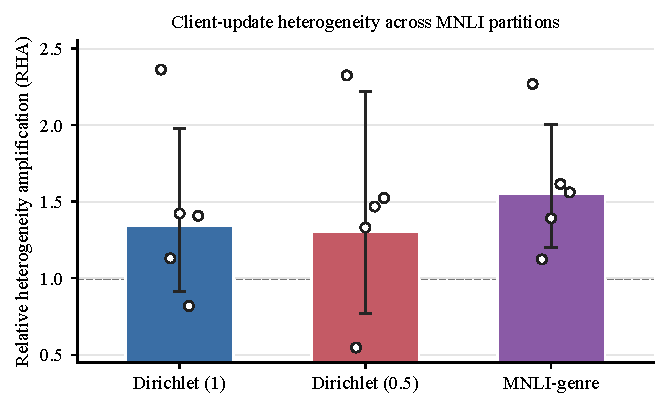
\includegraphics[width=\linewidth]
				{rha_partition_summary.pdf}
				\caption{Overall relative heterogeneity amplification.}
				\label{fig:rha-summary}
			\end{subfigure}
			
			% (b) Query projection
			\begin{subfigure}[t]{0.47\textwidth}
				\centering
				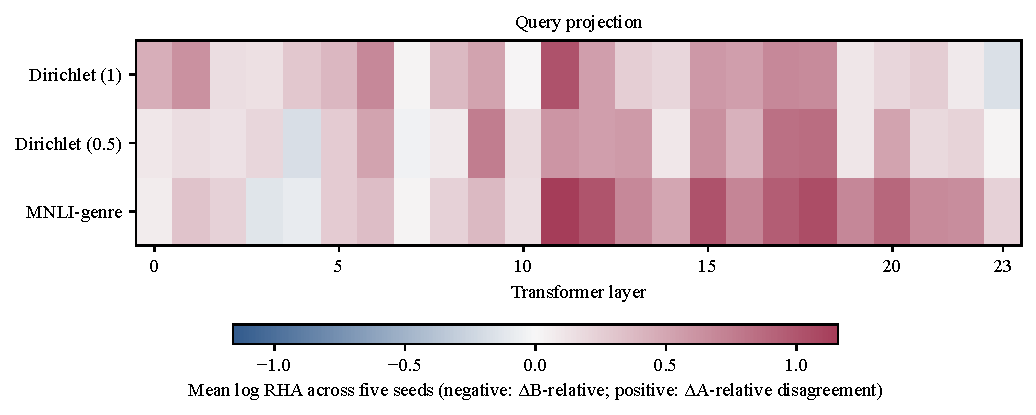
\includegraphics[width=\linewidth]
				{rha_query_layerwise.pdf}
				\caption{Layer-wise RHA for the query projection.}
				\label{fig:rha-query}
			\end{subfigure}
			% (c) Value projection
			\hfill
			\begin{subfigure}[t]{0.47\textwidth}
				\centering
				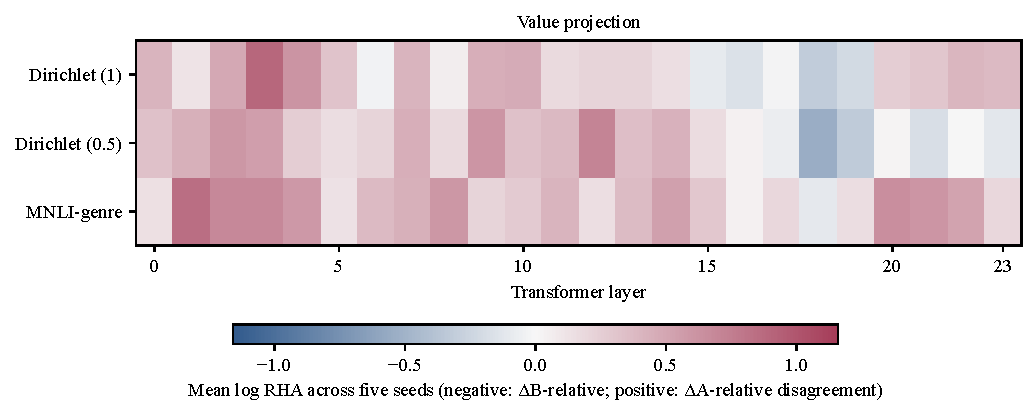
\includegraphics[width=\linewidth]
				{rha_value_layerwise.pdf}
				\caption{Layer-wise RHA for the value projection.}
				\label{fig:rha-value}
			\end{subfigure}
			
			\caption{
				Relative heterogeneity amplification of LoRA factors across
				MNLI client partitions.
				The clients perform local training independently without server
				aggregation. For each of the three non-IID partitioning schemes,
				five three-client partitions are independently generated using
				different partition seeds. Each non-IID partition is paired with an
				IID reference partition generated using the same seed, while the model
				initialization and training-related random seeds are fixed across all
				partition instances.
				(a) Bars show the geometric mean across the five partition
				instances, white circles denote individual partition instances, and
				error bars represent one sample standard deviation in log-RHA space.
				The dashed line marks $\mathrm{RHA}=1$.
				(b,c) Layer-wise mean log RHA for the query and value
				projections, respectively. Both heatmaps use the same color scale;
				positive values indicate stronger relative disagreement in
				$\Delta A$, whereas negative values indicate stronger relative
				disagreement in $\Delta B$.
			}
			\label{fig:mnli-rha}
		\end{figure*}
		



\end{document}
